% documentclass options:
\documentclass[11pt,
  a4paper,
  parskip=half, % This is some extra vertical space between paragraphs, the suggestion is 2cm which is really ugly, so we use what koma script gives us
  % you can also set it to full for even more space. But there is a bad tex style decision: parskip also changes the spacing between listitems such as
  % enumerate and itemize. For this purpose we include the enumitem package and set itemsep=.5em, of course you can change this
  BCOR=10mm, % BCOR is binding correction
  ngerman,
  % if you'd rather have a one sided thesis, add `oneside' to the documentclass
  % oneside,
  % ngerman is needed for hyphenation if the thesis contains parts written in German, switch order with english if you write mainly in English.
  % Remember to change order in the babel package (below) as well.
  % Last language is the preferred one.
  english]{scrbook}
\usepackage[ngerman, english]{babel} % If you write mainly in English change order to ngerman, english. Also change that in the documentclass options above.
% Include of titling must happen before \title etc.
% that's why it's not in setup.tex
\usepackage{titling}
\title{Expanding Action Space in Reinforcement Learning through Latent Models: A 2D Inverse Kinematics Benchmark}
\author{Robin Uhrich}

% Change to your first examiner
% The ~ enables non sentence spacing after a period
\newcommand{\firstexaminer}{Prof.~Dr.~Joschka Boedecker}
% Change to your second examiner, some undergraduate studies don't have a second examiner
% in this case just comment out the following line
\newcommand{\secondexaminer}{Prof.~Dr.~Wile E. Coyote}
% Change to your adivers
\newcommand{\advisers}{Jasper Hoffman}

% include all packages and define commands in setup.tex

%------------------------------------------------------------------------------
%       package includes
%------------------------------------------------------------------------------
    % font encoding is set up for pdflatex, for other environments see
    % http://tex.stackexchange.com/questions/44694/fontenc-vs-inputenc
    \usepackage[T1]{fontenc}  % 8-bit fonts, improves handling of hyphenations
    % provides `old' commands for table of contents. Eases the ability to switch
    % between book and scrbook
    \usepackage{scrhack}


    % ------------------- layout, default -------------------
    % adjust the style of float's captions, separated from text to improve readabilty
    \usepackage[labelfont=bf, labelsep=colon, format=hang, textfont=singlespacing]{caption}
    % With format = hang your caption will look like this:
    % Figure 1: Lorem ipsum dolor sit amet,
    %           consectetuer adipiscing elit.
    %           Ut purus elit, vestibulum
    % If you instead want
    % Figure 1: Lorem ipsum dolor sit amet,
    % consectetuer adipiscing elit. Ut purus
    % elit, vestibulum
    % change to format=plain
    \usepackage{chngcntr}  % continuous numbering of figures/tables over chapters
    \counterwithout{equation}{chapter}
    \counterwithout{figure}{chapter}
    \counterwithout{table}{chapter}

    % Uncomment the following line if you switch from scrbook to book
    % and comment the setkomafont line
    %\usepackage{titlesec}  % remove "Chapter" from the chapter title
    %\titleformat{\chapter}[hang]{\bfseries\huge}{\thechapter}{2pc}{\huge}
    \setkomafont{chapter}{\normalfont\bfseries\huge}

    \usepackage{setspace}  % Line spacing
    \onehalfspacing
    % \doublespacing  % uncomment for double spacing, e.g. for annotations in correction

    % ------------------- functional, default-------------------
    \usepackage[dvipsnames]{xcolor}  % more colors
    \usepackage{array}  % custom format per column in table - needed on the title page
    \usepackage{graphicx}  % include graphics
    \usepackage{subfig}  % divide figure, e.g. 1(a), 1(b)...
    \usepackage{amsmath}  % |
    \usepackage{amsthm}   % | math, bmatrix etc
    \usepackage{amsfonts} % |
    \usepackage{calc}  % calculate within LaTeX
    \usepackage[unicode=true,bookmarks=true,bookmarksnumbered=true,
                bookmarksopen=true,bookmarksopenlevel=1,breaklinks=false,
                pdfborder={0 0 0},backref=false,colorlinks=false]{hyperref}
    \usepackage{etoolbox} % if-else commands


    %==========================================
    % You might not need the following packages, I only included them as they
    % are needed for the example floats
    % ------------------- functional, custom -------------------
    \usepackage{algorithm,algpseudocode}
    \usepackage{bm}  % bold greek variables (boldmath)
    \usepackage{tikz}
    \usetikzlibrary{positioning}  % use: above left of, etc
    
    % Required for the ToDo list.
    \usepackage{ifthen}

    % Improves general appearance of the text
    \usepackage[protrusion=true,expansion=true, kerning]{microtype}
    \usepackage{enumitem}
    % Nicer font for pdf rendering.
    %\usepackage{lmodern}
    
    % For nicer looking tables.
    \usepackage{booktabs}

    % You don't need this, just for demonstration of a longer caption.
    \usepackage{lipsum}

%------------------------------------------------------------------------------
%       (re)new commands / settings
%------------------------------------------------------------------------------
    % ----------------- referencing ----------------
    \newcommand{\secref}[1]{Section~\ref{#1}}
    \newcommand{\chapref}[1]{Chapter~\ref{#1}}
    \renewcommand{\eqref}[1]{Equation~(\ref{#1})}
    \newcommand{\figref}[1]{Figure~\ref{#1}}
    \newcommand{\tabref}[1]{Table~\ref{#1}}
    \newcommand{\algoref}[1]{Algorithm~\ref{#1}}

    % ------------------- colors -------------------
    \definecolor{darkgreen}{rgb}{0.0, 0.5, 0.0}
    % Colors of the Albert Ludwigs University as in
    % https://www.zuv.uni-freiburg.de/service/cd/cd-manual/farbwelt
    \definecolor{UniBlue}{RGB}{0, 74, 153}
    \definecolor{UniRed}{RGB}{193, 0, 42}
    \definecolor{UniGrey}{RGB}{154, 155, 156}


    % ------------------- layout -------------------
    % prevents floating objects from being placed ahead of their section
    \let\mySection\section\renewcommand{\section}{\suppressfloats[t]\mySection}
    \let\mySubSection\subsection\renewcommand{\subsection}{\suppressfloats[t]\mySubSection}



    % ------------------- math formatting commands -------------------
    % define vectors to be bold instead of using an arrow
    \renewcommand{\vec}[1]{\mathbf{#1}}
    \newcommand{\mat}[1]{\mathbf{#1}}
    % tag equation with name
    \newcommand{\eqname}[1]{\tag*{#1}}


    % ------------------- pdf settings -------------------
    % ADAPT THIS
    \hypersetup{pdftitle={\thetitle},
                pdfauthor={\theauthor},
                pdfsubject={Undergraduate thesis at the Albert Ludwig University of Freiburg},
                pdfkeywords={deep learning, awesome algorithm,  undergraduate thesis},
                pdfpagelayout=OneColumn, pdfnewwindow=true, pdfstartview=XYZ, plainpages=false}


    %==========================================
    % You might not need the following commands, I only included them as they
    % are needed for the example floats

    % ------------------- Tikz styles -------------------
    \tikzset{>=latex}  % arrow style

    % --------------------- tables ----------------------
    \newcolumntype{L}{>{$}l<{$}}
    
    % ------------------- algorithm ---------------------
    % Command to align comments in algorithm
    \newcommand{\alignedComment}[1]{\Comment{\parbox[t]{.35\linewidth}{#1}}}
    % define a foreach command in algorithms
    \algnewcommand\algorithmicforeach{\textbf{foreach}}
    \algdef{S}[FOR]{ForEach}[1]{\algorithmicforeach\ #1\ \algorithmicdo}

    % line spacing should be 1.5
    \renewcommand{\baselinestretch}{1.5}

    % set distance between items in a list, for more details see the
    % enumitem package: https://www.ctan.org/pkg/enumitem
    \setlist{itemsep=.5em}
    
    % use ra in your tables to increase the space between rows
    % 1.3 should be fine
    \newcommand{\ra}[1]{\renewcommand{\arraystretch}{#1}}

	% ToDo counters
	\usepackage{ifthen} %für whiledo-Schleife
	\newcounter{todos}
	\setcounter{todos}{0}
	\newcounter{extends}
	\setcounter{extends}{0}
	\newcounter{drafts}
	\setcounter{drafts}{0}

	% ------------------- marker commands -------------------
    % ToDo command
    \newcommand{\todo}[1]{\textbf{\textcolor{red}{(TODO: #1)}}\refstepcounter{todos}\label{todo \thetodos}}
	\newcommand{\extend}[1]{\textbf{\textcolor{darkgreen}{(EXTEND: #1)}}\refstepcounter{extends}\label{extend \theextends}}
	% Lighter color to note down quick drafts
	\newcommand{\draft}[1]{\textbf{\textcolor{NavyBlue}{(DRAFT: #1)}}\refstepcounter{drafts}\label{draft \thedrafts}}
	
	% microtype with lmodern, see https://tex.stackexchange.com/questions/75305/microtype-warning-with-lmodern-package-and-koma-script
	%\DeclareMicrotypeAlias{lmss}{cmr}


\begin{document}
    \pagestyle{empty} % no header and no page number
    % disable hyper links to remove warning "destination with same identifier"
    % this means within this section nothing can be referenced with a hyperlink
    \hypersetup{pageanchor=false}

    % enable/disable, depending on your chosen language
    
\begin{titlepage}
\begin{center}

\newcommand{\HorizontalLine}{\rule{\linewidth}{0.3mm}}

{\Large Undergraduate/Master's Thesis}\\[1.3cm]


% _____________________________________________________________________________
\HorizontalLine \\[0.4cm]
% Write your title in a fancy way like this if you want to customize it, otherwise simply let tex do it for you
% \begin{spacing}{3}
%     {\huge \bfseries The Long, Long } \\
%     {\huge \bfseries Long Long} \\
%     {\huge \bfseries Title}\\
% \end{spacing}
{ \huge \bfseries \thetitle }
\HorizontalLine \\[1.5cm]
% _____________________________________________________________________________


{\Huge \theauthor} \\[2cm]


\begin{tabular}[hc]{>{\huge}l >{\huge}l}
  Examiner: & \firstexaminer \\[0.3cm]
  Advisers: & \advisers \\[1.2cm]
\end{tabular}
\vfill  % move the following text to the bottom

\Large {
    University of Freiburg\\
    Faculty of Engineering\\
    Department of Computer Science\\
    Neurobotics Lab\\[1cm]

    \today
    \\
}
\end{center}
\end{titlepage}

\thispagestyle{empty}
% title page back
\ \vfill \ \\  % at least one space required before vfill
\
\textbf{Writing Period}            \smallskip{} \\
05.\,07.\,2016 -- 05.\,10.\,2016   \bigskip{} \\
\
\textbf{Examiner}                  \smallskip{} \\
\firstexaminer                     \bigskip{} \\
\
% If there is a second examiner include it
\ifdef{\secondexaminer}
	{
	% Include
	\textbf{Second Examiner}       \smallskip{} \\
	\secondexaminer                \bigskip{} \\
	\
	}
	{
	% No second examiner, ignore
	}
\textbf{Advisers}                  \smallskip{} \\
\advisers

    \begin{titlepage}
\begin{center}

\newcommand{\HorizontalLine}{\rule{\linewidth}{0.3mm}}

{\Large Bachelor Thesis}\\[1.3cm]


% _____________________________________________________________________________
\HorizontalLine \\[0.4cm]
% Write yourtitle in a fancy way like this if you want to customize it, otherwise simply let tex do it for you
% \begin{spacing}{3}
%     {\huge \bfseries Der Lange, Lange } \\
%     {\huge \bfseries Lange Lange} \\
%     {\huge \bfseries Titel}\\
% \end{spacing}
{ \huge \bfseries \thetitle }
\HorizontalLine \\[1.5cm]
% _____________________________________________________________________________


{\Huge \theauthor} \\[2cm]


\begin{tabular}[hc]{>{\huge}l >{\huge}l}
  Gutachter: & \firstexaminer \\[0.3cm]
  Betreuer: & \advisers \\[1.2cm]
\end{tabular}
\vfill  % move the following text to the bottom

\Large {
    Albert-Ludwigs-Universität Freiburg\\
    Technische Fakultät\\
    Institut für Informatik\\
    Lehrstuhl für Neurorobotik\\[1cm]

    \today
    \\
}
\end{center}
\end{titlepage}

\thispagestyle{empty}
% title page back
\ \vfill \ \\  % at least one space required before vfill
\
\textbf{Bearbeitungszeit}            \smallskip{} \\
05.\,07.\,2016 -- 05.\,10.\,2016   \bigskip{} \\
\
\textbf{Gutachter}                  \smallskip{} \\
\firstexaminer                      \bigskip{} \\
\
% If there is a second examiner include it
\ifdef{\secondexaminer}
	{
	% Include
	\textbf{Zweitgutachter}        \smallskip{} \\
	\secondexaminer                \bigskip{} \\
	\
	}
	{
	% No second examiner, ignore
	}
\textbf{Betreuer}                  \smallskip{} \\
\advisers

    \pagestyle{plain} % remove chapter name from top, page number at the bottom
    % use \pagestyle{headings} for having the chapter on top of the pages
    % if you wang a more fancy header use \usepackage[automark,headsepline]{scrlayer-scrpage}
    % and read about it in the KOMA script documentation, https://www.ctan.org/pkg/koma-script
    \frontmatter  % roman page numbers
    % Copied from the official declaration from the examination office (typos fixed).
% Please double check the wording on their website and report changes.
% (https://www.tf.uni-freiburg.de/de/studium-lehre/a-bis-z-studium/dokumente/Declarationforthefinalthesis.pdf)

\chapter*{Declaration}

I hereby declare that I am the sole author and composer of my thesis and that no other sources or learning aids, other than those listed, have been used. Furthermore, I declare that I have acknowledged the work of others by providing detailed references of said work.  \newline
I hereby also declare that my Thesis has not been prepared for another examination
or assignment, either wholly or excerpts thereof.
\\[3\normalbaselineskip]
\begin{tabular}{p{\textwidth/2} l}
  \rule{\textwidth/3}{0.4pt}   &   \rule{\textwidth/3}{0.4pt} \\
  Place, Date                  &   Signature
\end{tabular}

    \chapter*{Abstract}
foo bar

\chapter*{Zusammenfassung}
German version is only needed for an undergraduate thesis.
    \tableofcontents
    \listoffigures
    \listoftables
    \listofalgorithms
    \hypersetup{pageanchor=true}  % re-enable hyperlinking

    \mainmatter{}  % Arabic page numbers
    \chapter{Introduction}\label{chap:introduction}



% This thesis explores the integration of latent models, including pre-trained Variational Autoencoder decoders and supervised models, into Reinforcement Learning frameworks. The objective is to expand the action space capabilities of RL agents. The research is evaluated using a benchmark environment: solving a 2D Inverse Kinematics problem on a robot arm with a variable number of joints $N$. The study investigates how the incorporation of latent models enhances the RL agent's performance in handling complex action spaces.

In the ever-evolving landscape of artificial intelligence and machine learning, Reinforcement Learning (RL) stands as a powerful paradigm for enabling autonomous agents to learn and adapt to their environments. RL has demonstrated remarkable success in a variety of applications, from game-playing agents \cite{SAC_VideoGames_Paper} to robotics control systems \cite{SAC_Applications_Paper} \cite{anymal_RL}. However, one of the enduring challenges in RL lies in the limitation of the action space—an agent's ability to act upon its environment. The dimensionality and complexity of the action space profoundly impact an agent's capacity to solve increasingly intricate tasks \cite{RL_Complex_Action_Spaces}.

This thesis explores a novel approach to address the action space limitations in RL by leveraging latent models. Specifically, it investigates the integration of pre-trained latent models, including Variational Autoencoder (VAE) decoders and supervised models, into RL frameworks. The primary aim is to empower RL agents to handle significantly more extensive and complex action spaces effectively. To evaluate the effectiveness of this approach, we developed a new scalable benchmark environment: the 2D Inverse Kinematics problem.

\textbf{The Challenge of Action Space in Reinforcement Learning}

The action space of an RL agent comprises the set of actions it can take to interact with its environment. In many real-world scenarios, especially those involving robotic systems and control tasks, the action space can be high-dimensional and continuous. Traditional RL algorithms often struggle to operate effectively in such settings due to the curse of dimensionality, making the exploration of all possible actions computationally infeasible.

This challenge has motivated researchers to seek innovative solutions that expand the boundaries of RL action spaces. The integration of latent models offers a promising avenue. These models can encode complex actions into lower-dimensional representations, enabling RL agents to navigate large action spaces more efficiently and effectively.

\textbf{The Role of Latent Models in Expanding Action Spaces}

Latent models, such as VAEs and supervised models, have demonstrated their prowess in capturing essential patterns and representations within data \cite{pml2Book}. By pre-training these models on relevant tasks, we can harness their latent spaces to transform high-dimensional action spaces into more compact and manageable forms. This, in turn, equips RL agents with the ability to explore and exploit action spaces that were previously deemed insurmountable.

\textbf{Benchmarking Progress: The 2D Inverse Kinematics Problem}

To assess the efficacy of integrating latent models into RL, we turn to the 2D Inverse Kinematics problem. This problem simulates the control of a multi-jointed robotic arm, where each joint represents a dimension in the action space. The challenge lies in determining the joint angles required to position the end effector at a specified target location. By scaling the complexity of this benchmark through varying the number of joints $N$, we can rigorously evaluate the impact of latent models on action space expansion.

\textbf{Structure of the Thesis}

This thesis is structured as follows: in \chapref{chap:background}, we provide an overview of the background for this research. \chapref{chap:relatedwork} delves into a comprehensive literature review, examining related work in RL, latent models, and their integration. \chapref{chap:Methodology} outlines the methodology used, including details on the latent models employed and their integration into RL. \chapref{chap:experiments} presents the experimental results and analysis from the 2D Inverse Kinematics benchmark. \chapref{chap:discussion} discusses experimental results and finally, \chapref{chap:conclusion} offers conclusions and outlines potential future directions for research in this domain.

The integration of latent models with RL to expand action space capabilities holds great promise for advancing the capabilities of autonomous agents. By addressing one of the core challenges in RL, this research aims to contribute to the broader field of artificial intelligence and robotics, opening doors to new possibilities in complex task execution and problem-solving.




% This is a template for an undergraduate or master's thesis.
% The first sections are concerned with the template itself. If this is your first
% thesis, consider reading \secref{sec:advice}.
% 
% The structure of this thesis is only an example.
% Discuss with your adviser what structure fits best for your thesis.
% 
% \section{Template Structure}
% \begin{itemize}
%     \item To compile the document either run the makefile or run your compiler on the file `thesis\_main.tex'. The included makefile requires latexmk which automatically runs bibtex and recompiles your thesis as often as needed. Also it automatically places all output files (aux, bbl, ...) in the folder `out'. As the pdf also goes in there, the makefile copies the pdf file to the parent folder. There is also a makefile in the chapters folder, to ensure you can also compile from this directory.
% 
%     \item The file `setup.tex' includes the packages and defines commands. For more details see \secref{sec:setup}.
% 
%     \item Each chapter goes into a separate document, the files can be found in the folder chapters.
% 
%     \item The bib folder contains the .bib files, I'd suggest to create multiple bib files for different topics. If you add some or rename the existing ones, don't forget to also change this in thesis\_main.tex. You can then cite as usual~\cite{kingma2014adam, bromley1993siamesesignature,muja2009flann}.
% 
%     \item The template is written in a way that eases the switch from scrbook to book class. So if you're not a fan of KOMA you can just replace the documentclass in the main file. The only thing that needs to be changed in setup.tex is the caption styling, see the comments there.
% \end{itemize}
% 
% 
% \section{setup.tex}\label{sec:setup}
% Edit setup.tex according to your needs. The file contains two sections, one for package includes, and one for defining commands. At the end of the includes and commands there is a section that can safely be removed if you don't need algorithms or tikz. Also don't forget to adapt the pdf hypersetup!!\\
% setup.tex defines:
% \begin{itemize}
%     \item some new commands for remembering to do stuff:
%     \begin{itemize}
%         \item \verb|\todo{Do this!}|: \todo{Do this!}
%         \item \verb|\extend{Write more when new results are out!}|:\\ \extend{Write more when new results are out!}
%         \item \verb|\draft{Hacky text!}|: \draft{Hacky text!}
%     \end{itemize}
% 
%     \item some commands for referencing, `in \verb|\chapref{chap:introduction}|' produces 'in \chapref{chap:introduction}'
%     \begin{itemize}
%         \item \verb|\chapref{}|
%         \item \verb|\secref{sec:XY}|
%         \item \verb|\eqref{}|
%         \item \verb|\figref{}|
%         \item \verb|\tabref{}|
%     \end{itemize}
% 
%     \item the colors of the Uni's corporate design, accessible with\\ \verb|{\color{UniX} Colored Text}|
%     \begin{itemize}
%         \item {\color{UniBlue}UniBlue}
%         \item {\color{UniRed}UniRed}
%         \item {\color{UniGrey}UniGrey}
%     \end{itemize}
% 
%     \item a command for naming matrices \verb|\mat{G}|, $\mat{G}$, and naming vectors \verb|\vec{a}|, $\vec{a}$. This overwrites the default behavior of having an arrow over vectors, sticking to the naming conventions  normal font for scalars, bold-lowercase for vectors, and bold-uppercase for matrices.
% 
%     \item named equations:
%         \begin{verbatim}
% \begin{align}
%     d(a,b) &= d(b,a)\\ \eqname{symmetry}
% \end{align}
%         \end{verbatim}
%         \begin{align}
%             d(a,b) &= d(b,a)\\ \eqname{symmetry}
%         \end{align}
% \end{itemize}
% 
% \section{Advice}\label{sec:advice}
% This section gives some advice how to write a thesis ranging from writing style to formatting. To be sure, ask your advisor about his/her preferences.\\
% For a more complete list we recommend to read Donald Knuth's paper on mathematical writing. (At least the first paragraph). \url{http://jmlr.csail.mit.edu/reviewing-papers/knuth_mathematical_writing.pdf}
% 
%     \begin{itemize}
% 
%         \item If you use formulae pay close attention to be consistent throughout the thesis!
% 
%         \item In a thesis you don't write `In [24] the data is..'. You have more space than in a paper, so write `AuthorXY et al. prepare the data... [24]'. Also pay attention to the placement: The citation is at the end of the sentence before the full stop with a no-break space. \verb|... last word~\cite{XY}.|
% 
%         \item Pay attention to comma usage, there is a big difference between English and German. `...the fact that bla...' etc.
% 
%         \item Do not write `don't ', `can't' etc. Write `do not', `can not'.
% 
%         \item If an equation is at the end of a sentence, add a full stop. If it's not the end, add a comma: {$a= b + c$~~~~(1),}
% 
%         \item Avoid footnotes if possible.
% 
%         \item Use \verb|``''| for citing, not \verb|""|.
% 
%         \item It's important to look for spelling mistakes in your thesis. There are also tools like aspell that can help you find such mistakes.
%         This is never an excuse not to properly read your thesis again, but it can help.
%         You can find an introduction under \url{https://git.fachschaft.tf/fachschaft/aspell}.
% 
%         \item If have things like a graph or any other drawings consider using tikz, if you need function graphs or diagrams consider using pgfplots.
%         This has the advantage that the style will be more consistent (same font, formatting options etc.) than when you use some external program.
% 
%         \item Discuss with your advisor whether to use passive voice or not. In most computer science papers passive voice is avoided. It's harder to read, more likely to produce errors, and most of the times less precise. Of course there are situations where the passive voice fits but in scientific papers they are rare. Compare the sentence: `We created the wheel to solve this.' to `The wheel was created to solve this', you don't know who did it, making it harder to understand what is your contribution and what is not.
%         
%         \item In tables avoid vertical lines, keep them clean and neat. See \ref{tab:accuracy} for an example. More details can be found in the `Small Guide to Making Nice Tables' \url{https://www.inf.ethz.ch/personal/markusp/teaching/guides/guide-tables.pdf}
% 
%     \end{itemize}
% 
    \chapter{Related Work}\label{chap:relatedwork}

In the following section we will briefly explain the already existing research regarding hwo previous research tackled the problem of inverse kinematics and how current research combines Latent models with reinforcement learning.

\section{Learning Operational Space Control}

The authors of ``Learning Operational Space Control''\cite{Learning_to_Control_in_Operational_Space}, Jan Peters and Stefan Schaal, present a novel approach for controlling the end-effector of a rigid robot arm. Using operational space control in robots meant to work safely in human environments is challenging due to unmodeled nonlinearities, leading to accuracy reduction and unpredictable behavior.\\
To address this challenge, learning control methods are explored. Traditional learning methods struggle to capture the structured knowledge required for operational space control, such as Jacobians and inertia matrices, which may not always be observable. This paper introduces novel approaches to learning operational space control, focusing on learning the operational space control law directly, similar to an inverse model learning problem. \\
Key insights for this project include the realization that a physically correct solution to the inverse problem with redundant degrees-of-freedom is attainable through piecewise linear learning. Additionally, many operational space controllers can be viewed as constrained optimal control problems. A learning algorithm is formulated to synthesize a globally consistent desired resolution of redundancy while learning the operational space controller, treated as a reinforcement learning problem maximizing an immediate reward.

\section{Motor synergy development in high-performing deep reinforcement learning algorithms}

In their paper ``Motor synergy development in high-performing deep reinforcement learning algorithms''\cite{Motor_Synergy_Learning} the researchers Jiazheng Chai and  Mitsuhiro Hayashibe investigate if the motor synergy concept could also be observed in deep reinforcement learning for robotics. The motor synergy concept states that a sets of actuators e.g. muscles in animals or motors in robots, are controlled by a reduced set of commands with respect to the degrees of freedom resembled by the actuators. They study this concept by training an agent either with SAC or TD3 on several benchmark environments like Half-Cheetah \cite{Half_Cheetah}, and further investigate if it is possible ot reduce the dimensionality of the collected control signal via principal component analysis \cite{PCA} and reconstruct it as close as possible to the original signal.


\section{LASER: Learning Latent Action Space for Efficient Reinforcement Learning}

In the paper ``LASER: Learning Latent Action Space for Efficient Reinforcement Learning'' from Arthur Allshire, Roberto Martín-Martín, Charles Lin, Shawn Manuel, Silvio Savarese and Animesh Gartg from 2021 \cite{LASER} the authors trained jointly a Soft Actor-Critic algorithm and a conditional Variational Autoencoder for robot manipulation. The authors split the problem into two sub-problems. First they lear a mapping $g(o): \mathcal{O} \to \bar{\mathcal{A}}$ from observation space into a latent space and second using a robot controller $f(\bar{a}): \bar{\mathcal{A}} \to \mathcal{A}$ to map their latent signals into actuation commands. Their algorithm LASER is trained as an encoder-decoder model which learns to map manifold of low-level commands to a latent action space. 

% \begin{figure}
%     \centering
%         
\includegraphics[width=0.46 \linewidth]{figures/place_holder.png}
%     \caption[LASER workflow]{Workflow of LASER approach. The image was adapted from \cite{LASER}}
%     \label{fig:LASER_workflow}
% \end{figure}
% 
% In \figref{fig:LASER_workflow} we can observer the proposed workflow. Important to note is that the Variational Autoencoder is trained either on data collected by a different policy (offline), like an expert or it is trained on the fly, using data generated by the policy and itself via variational inference. 


\section{CALM: Conditional Adversarial Latent Models for Directable Virtual Characters}

Researchers from NVIDIA  Chen Tessler et.al. have developed Conditional Adversarial Latent Models (CALM)  in the paper ``CALM: Conditional Adversarial Latent Models for Directable Virtual Characters''\cite{CALM} to enable users to direct the behavior of virtual characters in interactive simulations. CALM combines imitation learning with a control policy and motion encoder to create a representation of human motion that is diverse and controllable. The key phases of CALM include:
\begin{enumerate}
    \item low-level training, where it learns a motion encoder and decoder
    \item directionality control, where a high-level policy guides motion direction and style
    \item and inference, where trained models are combined to compose complex character movements using a finite-state machine
\end{enumerate}
This approach allows users to intuitively control virtual characters, making it applicable for interactive applications like video games.
    \chapter{Background}\label{chap:background}

The following part is to provide a short introduction into the theory of reinforcement learning, the Soft Actor Critic Algorithm (SAC) as well to Variational Autoencoders (VAE) and Conditional Variational Autoencoders (CVAE).
\todo{update!!!}

\section{RL Framework}\label{sec:RL-Framework}

Learning is a topic that is present in all our lives since their beginning. We all learn to move our arms, like an infant that is wiggling around, learn to walk, to speak and more or less any other skill that we find in our personal repository until now.  

Reinforcement Learning (RL) is about to have a computational approach to this kind of learning.
In the class of RL-Problems the environment provides a challenge like, riding a bicycle. But it is not told how this goal can be achieved.  Therefore it has be learned how to derive actions from situations on or off the bike in order to complete this task or - speaking of the numerical approach - maximize a reward function.
In most cases the problem solving methods that are classified as RL-methods are applied on tasks that require not only a sequence of actions to interact with an environment but also some kind of feedback.
Therefore these setups are designed to provide this kind of feedback. Either if it is an immediate feedback like an additional time step the agent has not crashed the bike or if it is more like a long shot feedback, for example a bonus that the agent has earned after winning board game. 
These principals can be boiled down to three main characteristics of reinforcement learning problems:

\begin{itemize}
    \item There is a closed loop mechanism between actions and feedback that is provided by the environment where the agent is operating in.
    \item The agent is not given any direct instructions how to solve the given problem.
    \item The actions an agent is performing have consequences over time. Either for him or the environment he is working in.  
\end{itemize}

Before we can have an exemplary look on the closed loop mechanics, we would like to introduce a couple of key components of RL including the Markov Decision Process.

% \begin{figure}
	\centering
	\minipage{0.5\textwidth}
    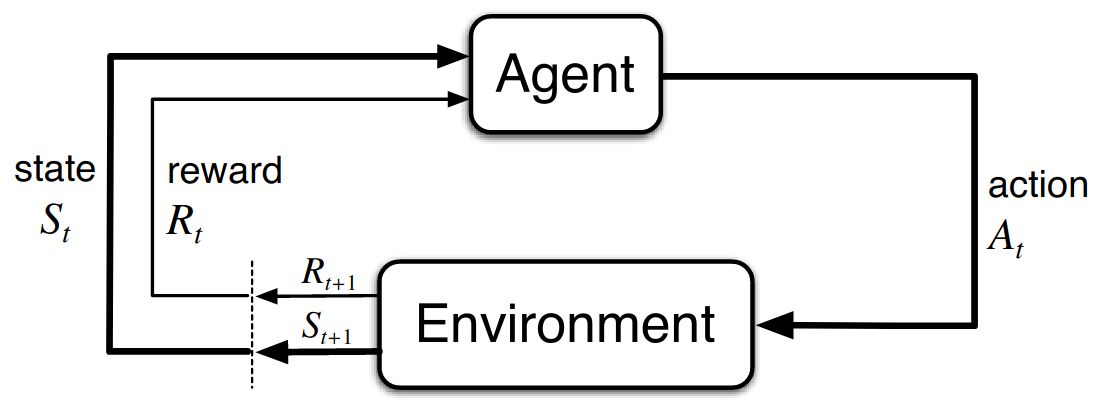
\includegraphics[width=\linewidth,]{figures/background/agent-environment-interaction.png}
	\caption{interaction between agent and the environment}
	\label{fig:agent-environment_interaction}
	\endminipage
\end{figure}



\begin{figure}
	\centering
	\minipage{0.5\textwidth}
    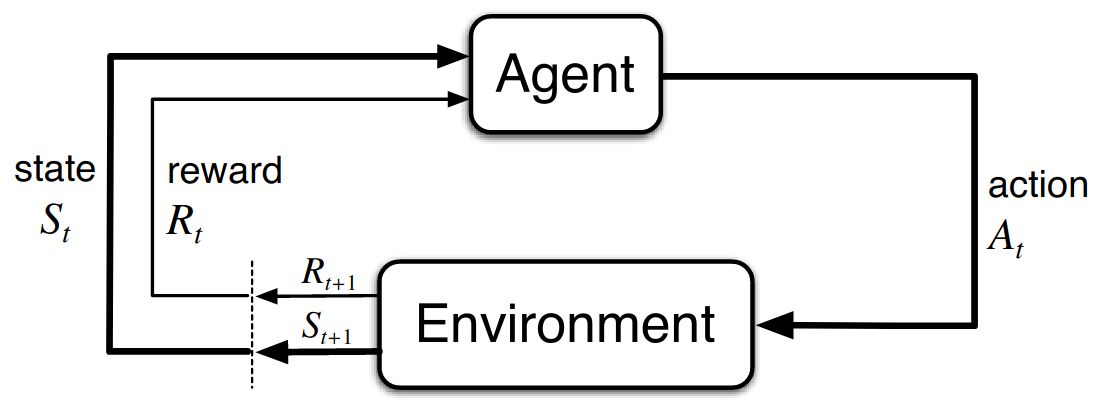
\includegraphics[width=\linewidth,]{figures/background/agent-environment-interaction.png}
	\caption{interaction between agent and the environment}
	\label{fig:agent-environment_interaction}
	\endminipage
\end{figure}
\todo{cite figure}


Every agent exists in a specified environment and also interacts within a sequence of discrete time steps $t \in \mathbb{N}$. In order to do so the agent has to perceive the environment through a \textbf{state} representation $S_t \in \mathcal{S}$ which is an element of all possible states, the state space $\mathcal{S}$. To really interact with the environment the agent has to perform an \textbf{action} $A_t \in \mathcal{A}(S_t)$ where $\mathcal{A}(S_t)$ is the set of all possible actions in given state $S_t$. To chose an action the agent calculates for each possible action $A_t$ a probability $\pi_{\theta, t}(A_t|S_t)$ for a given state $S_t$ and chooses the maximum with respect to the given actions. To achieve a more compact notation we will refer to the action $A_t = a$ and the state $S_t = s$. To avoid confusions with the number $\pi \approx 3.141$ we refer to the policy always as a parameterized policy $\pi_\theta = \pi_{\theta, t}(a|s)$.  
This probability distribution is called the \textbf{policy}. 
After the agent has chosen and executed an action, which also means the environment will move one time step further $t \to t + 1$, the environment will return the next state $S_{t+1}$ and the agent will perceive a \textbf{reward} $R_{t+1} \in \mathbb{R}$ with $\mathbb{R}$ as the set of all possible rewards.\\
The long term goal of the agent is to adapt its policy to maximize the total amount reward the agent receives from the environment.
These key terminology can also be found in the notation of a Markov Decision Process which is classified as a 4-Tuple of: $(\mathcal{S}, \mathcal{A}, P_a(s, s'), R_a(s, s'))$ with $ P_a(s, s')$ as a probability distribution that action $a$ in state state $s$ will lead to the next state $s' = s_{t+1}$ and $ R_a(s, s')$ as reward function for transitioning from $s$ to $s'$ with $a$.

\todo{
Explain the concept of reinforcement learning and its applications
Describe the Markov decision process (MDP) and the Bellman equation
Discuss the challenges of using reinforcement learning in practice}

\todo{Es wird gern gesehen: Optimal value function optimal policy / Tradeoff, Sutton Barto. Generalized Policy iteration. Es geht darum einaml ne policy und ne value function zu fnden, Bellman equations}

The overall goal of an agent is to maximize its received cumulative return $G_t$ for one run until time step $T$. This is metric is denoted in \eqref{eqn:discounted-cumulative-return}. In \eqref{eqn:discounted-cumulative-return} $\gamma$ is the discount rate, $0 \leq \gamma \leq 1$, a parameter to regularize the \textit{importance} of individual received rewards over time. 

\todo{cite sutton barto}

\begin{align}
	G_t & \ \dot{=} \sum_{k=t+1}^T \gamma^{k-t-1}R_k \label{eqn:discounted-cumulative-return} \\
	&= R_{t+1} + \gamma G_{t+1} \label{eqn:discounted-cumulative-return-recursive}
\end{align}

Unfortunately the individual rewards $R_t$ are highly dependent on state action pairs in the future, so they are not accessible at the current time step. To solve this problem reinforcement algorithms are trying to maximize the expected return $v_{\pi_\theta}(s)$ as in \eqref{eqn:expected-return}, or value function, for a given state. For Markov decision process we can define the value function as in \eqref{eqn:Bellman-valuefunction}. 

\todo{cite sutton barto}

\begin{align}
	% v_{\pi_\theta}(s) = \sum_a \pi_\theta(a|s) \sum_{s', r} P(s', r| s, a)\left[r + \gamma v_{\pi_\theta}(s'm)\right] 
	v_{\pi_\theta}(s) & \ \dot{=} \ \mathbb{E}_{\pi_\theta}[G_t | S_t = s] \label{eqn:expected-return} \\
	&\overset{\mathclap{\strut(\ref{eqn:discounted-cumulative-return-recursive})}}{=} \mathbb{E}_{\pi_\theta}[R_{t+1} + \gamma G_{t+1}| S_t = s] \nonumber \\
	& = \sum_a \pi_\theta(a|s) \sum_{s'} \sum_r P(s', r| s, a)\left[r + \gamma \mathbb{E}_{\pi_\theta}[G_{t+1} | S_{t+1} = s']\right] \nonumber \\
	& = \sum_a \pi_\theta(a|s) \sum_{s', r} P(s', r| s, a)\left[r + \gamma v_{\pi_\theta}(s'm)\right] \label{eqn:Bellman-valuefunction}
\end{align}

For a finite Markov decision process we can also find a the optimal value function $v_*(s)$ with respect to the optimal policy in \eqref{eqn:Bellman-optimal-valuefunction}. 

\begin{equation}\label{eqn:Bellman-action-valuefunction}
	q_{\pi_\theta}(s, a) = \sum_{s', r} P(s', r |s, a) \left[r + \gamma \sum_{a'} \pi_\theta(a'| s')q_{\pi_\theta}(s', a')\right]
\end{equation}

\begin{align}
	v_*(s) & \ \dot{=} \max_{\pi_\theta} v_{\pi_\theta}(s) \label{eqn:optimal-valuefunction} \\
	&=\max_a \sum_{s', r} P(s', r| s, a)[r + \gamma v_*(s')] \label{eqn:Bellman-optimal-valuefunction}
\end{align}

Because \eqref{eqn:optimal-valuefunction} holds this implies the reinforcement learning problem in \eqref{eqn:RL-policy-problem} for the optimal policy $\pi_\theta^*$ and a performance measure $J(\pi_\theta) = \mathbb{E}_{\pi_\theta}[G_t | S_t = s]$ as following:
\begin{align}
	\pi_\theta^* &= \arg \max_{\pi_\theta}J(\pi_\theta) \label{eqn:RL-policy-problem} \\
	&= \arg \max_{\pi_\theta} \mathbb{E}_{\pi_\theta}[G_t | S_t = s] \\
	&\overset{\mathclap{\strut(\ref{eqn:expected-return})}}{=} \arg \max_{\pi_\theta} v_{\pi_\theta}(s) \label{eqn:RL-policy-valuefunction}
\end{align}

\begin{equation}\label{eqn:Bellman-optimal-action-valuefunction}
	q_*(s, a) = \sum_{s', r} P(s', r|s, a)\left[r + \gamma \max_{a'} q_*(s', a')\right]
\end{equation}

\section{Generalized Policy Iteration}\label{sec:Generalized-Policy-Iteration}

This section is about to provide an introduction to the idea of policy iteration. For a more detailed look into the topic it is recommended refer to the Reinforcement Learning Textbook from Richard Sutton and Andrew Barto.

One fundamental concept for reinforcement learning algorithms is policy iteration. At Its core it is described as the alternating interaction between a policy improvement step and a policy evaluation step as in \figref{fig:policy-iteration-concept}. This interaction goes back and forth during the execution of most reinforcement learning algorithms until a state of convergence in the value function and policy has arrived. That means both value function and policy are optimal for the given problem. This state can be reached if the ``value function is consistent with the current policy, and the policy stabilizes only when it is greedy with respect to the current value function''. This can be also seen in the Bellman optimally equation as in \eqref{eqn:Bellman-optimal-valuefunction}. 

% \begin{figure}
    \begin{center}
        
\includegraphics[width=0.5\linewidth]{figures/place_holder.png}
        \caption[policy iteration concept]{\textbf{schematic drawing of a conditional Variational Autoencoder}}
        \label{fig:policy-iteration-concept}
    \end{center}
\end{figure}
\begin{figure}
    \begin{center}
        
\includegraphics[width=0.5\linewidth]{figures/place_holder.png}
        \caption[policy iteration concept]{\textbf{schematic drawing of a conditional Variational Autoencoder}}
        \label{fig:policy-iteration-concept}
    \end{center}
\end{figure}

We can also think about this process as a tradeoff between improving the policy towards an optimal greedy behavior which makes the value function incorrect (blue arrows indicate a policy improvement step) and adapting the value function with respect to the current policy which makes the policy automatically less optimal (red arrows indicate a policy evaluation step). \todo{Why?} Despite this tradeoff the algorithm tends to find an optimal solution for the policy and the value function in the long run. \todo{Where is the proof}

% \begin{figure}
    \begin{center}
        
\includegraphics[width=0.5\linewidth]{figures/place_holder.png}
        \caption[policy iteration funnel]{Figure shows the policy iteration funnel. The red arrows are a symbolic policy improvement step which is moving away from a precise value function. The blue arrows are a symbolic policy evaluation step which is moving the current policy further away from a greedy and thus stable policy. Both criterions are moving over time closer together until convergence with the optimal policy $\pi_*$ and the optimal value function $v_*$}
        \label{fig:policy-iteration-concept-funnel}
    \end{center}
\end{figure}
\begin{figure}
    \begin{center}
        
\includegraphics[width=0.5\linewidth]{figures/place_holder.png}
        \caption[policy iteration funnel. The red arrows are a symbolic policy improvement step which is moving away from a precise value function. The blue arrows are a symbolic policy evaluation step which is moving the current policy further away from a greedy and thus stable policy. Both criterions are moving over time closer together until convergence with the optimal policy $\pi_*$ and the optimal value function $v_*$]{\textbf{schematic drawing of a conditional Variational Autoencoder}}
        \label{fig:policy-iteration-concept-funnel}
    \end{center}
\end{figure}

\section{Soft Actor Critic}\label{sec:SAC}
% Briefly explain what the SAC algorithm is and why it is important
% Provide a preview of what the chapter will cover

Soft Actor-Critic was introduced by \todo{cite paper} in \todo{year}. It is an algorithm belonging to the family of model free, off-policy, actor-critic reinforcement learning algorithms. The family of actor-critic algorithms addresses challenges in exploration and sample efficiency. Similar to  other actor-critic algorithms it also employs the alternating concept of a policy improvement step and a policy evaluation step. In contrast to other actor-critic algorithms like XXXX \todo{fill} it uses the concept of entropy regularization and uses a stochastic policy for promoting exploration in the reinforcement learning environment. 
By jointly optimizing the policy and value functions using the maximum entropy objective enabled by entropy regularized, SAC effectively explores the environment while seeking to maximize rewards. This approach results in robust and adaptive policies that can efficiently handle various RL tasks. \todo{examples by paper }

In this section will introduce the concept of actor-critic algorithms, provide a detailed description of the SAC algorithm architecture, including entropy regularization and explain how to train the algorithm under the maximum entropy objective. 

% L1 smooth loss for $x, y \in \mathbb{R}$
% \begin{equation}
%     \mathcal{L}_\beta(x_i, y_i) = \begin{cases} \frac{1}{2 \beta} \cdot (x_i - y_i)^2 & \text{if $|x_i - y_i| < \beta$} \\ |x_i - y_i| -  \frac{\beta}{2} & \text{else}\end{cases} \\ 
% \end{equation}

\subsection{Actor-Critic Algorithms}

% Describe the basic actor-critic architecture and its limitations
% Explain the difference between on-policy and off-policy learning
% Describe the advantage of using a critic in the actor-critic algorithm
The basic actor-critic architecture is a type of reinforcement learning algorithm that consists of two components: an actor and a critic. The actor also referred to as the policy $\pi_\theta$ is responsible for selecting actions based on the current state, while the critic also referred to as a value function $v_{\pi_\theta}$ or a state value function $q_{\pi_\theta}$, evaluates the quality of the actor's actions by estimating the expected return. Like as introduced in \secref{sec:Generalized-Policy-Iteration} the actor uses the feedback from the critic to adjust its policy and improve its performance.

\todo{Maybe in RL Formulation or a separated section?}
One additional factor to distinguish between reinforcement learning algorithms and also actor-critic algorithms is by either on-policy learning or off-policy learning. On-policy learning or off-policy learning refer to different methods for updating the policy in reinforcement learning. In on-policy learning, the agent learns from the data generated by its current policy, while in off-policy learning, the agent learns from data generated by a different policy. On-policy learning can be more stable, but it may require more data to converge. Off-policy learning can be more efficient, but it can be more sensitive to the quality of the data.
\todo{cite sutton barto}

The advantage of using a critic in the actor-critic algorithm is: it provides a more stable feedback signal than using only rewards. The critic estimates the expected return from a state, for the value function, or a state action pair for the action-value function, which takes into account the long-term consequences of actions. This allows the actor to learn from the critic's feedback and improve its performance more efficiently than if it only received reward signals. Additionally, the critic can help to generalize across different states and actions, improving the overall performance of the algorithm.

One limitation of the basic actor-critic architecture is that it can suffer from high variance and slow convergence due to the interaction between the actor and critic. This can be addressed through the use of techniques such as baseline subtraction and eligibility traces.
\todo{look for paper}
\todo{cite sutton barto}

Popular examples for actor critic algorithms are:
\begin{itemize}
	\item Deep Deterministic Policy Gradient
	\item Soft Actor-Critic
	\item Proximal Policy optimization
\end{itemize}


% Explain the concept of entropy regularization and its role in the SAC algorithm
% Describe the architecture of the SAC algorithm and how it differs from traditional actor-critic algorithms
% Explain how the actor and critic are trained using the maximum entropy objective
% Discuss the advantages of the SAC algorithm, such as improved sample efficiency and exploration

\subsection{Entropy Regularization}\label{sec:entropy-regularization}

Entropy regularization is a policy regularization technique by incorporating the policy entropy, used to encourage the policy to explore a diverse range of actions during training. In SAC, entropy regularization is achieved by adding the entropy $H(\pi_\theta)$ as in \eqref{eqn:policy-entropy} to the policy objective function in \eqref{eqn:policy-update}.

\begin{align}
	H(\pi_\theta) &= \underset{s\sim\mathcal{S}, a\sim\mathcal{A}}{\mathbb{E}}\left[- \log(\pi_\theta(a|s))\right] \nonumber \\
	&= -\log(\pi_\theta(a|s)) \label{eqn:policy-entropy}
\end{align} \todo{is this correct?} \todo{something has to be cleared up with $H(\pi_\theta) != H(\pi_\theta(\cdot|s))$}

Including entropy into the objective function encourages the policy to generate actions with higher entropy (higher randomness), leading to more exploration, possibly accelerate training and preventing converging to a poor local optimum. \todo{cite: spinning up open ai} 

The randomness or uncertainty of a policy for a given state action pair $\pi_\theta(a|s)$ can be computed  by seeing  $\pi_\theta(a|s)$ as a density function and taking $\pi_\theta(\cdot|s) = \mathcal{N}\left(\mu(\pi_\theta(\cdot|s)), \sigma(\pi_\theta(\cdot|s))\right)$ as a parameterized normal distribution from which the action $a \sim \pi_\theta(\dot|s)$ is sampled. Therefor it possible to acquire the probability $\pi_\theta(a|s)$ of an action $a$ with as in \eqref{eqn:Gauss-Prob-Policy}.

\begin{align}
	\pi_\theta(a|s) = \frac{1}{\sigma(\pi_\theta(\cdot|s)) \sqrt{2\pi}} \exp\left(-\frac{1}{2}\frac{(a -\mu(\pi_\theta(\cdot|s)))^2}{\sigma(\pi_\theta(\cdot|s))^2}\right) \label{eqn:Gauss-Prob-Policy}
\end{align}

As a result of entropy regularization in each time step both value function $v_{\pi_\theta}$ and action-valuefunction $q_{\pi_\theta}$ become affected and turn into their counterpart $v_{\pi_\theta, H}$ and $q_{\pi_\theta, H}$ in \eqref{eqn:valuefunction-entropy-reg} and \eqref{eqn:action-valuefunction-entropy-reg} below.  Note that \eqref{eqn:action-valuefunction-entropy-reg-recursive} is the recursive version of \eqref{eqn:action-valuefunction-entropy-reg}.

\begin{align}
	v_{\pi_\theta, H}(s) &= \underset{\tau\sim\pi_\theta}{\mathbb{E}}\left[\sum_{t=0}^T\gamma^t\left(R_t + \alpha H(\pi_\theta(\cdot|s_t))\right)\mid s_0 = s\right]\label{eqn:valuefunction-entropy-reg} \\
	q_{\pi_\theta, H}(s, a) &= \underset{\tau\sim\pi_\theta}{\mathbb{E}}\left[\sum_{t=0}^T\gamma^t R_t + \alpha \sum_{t=1}^T \gamma^t H(\pi_\theta(\cdot|s_t))\mid s_0 = s, a_0=a\right]\label{eqn:action-valuefunction-entropy-reg} \\
	&= \underset{s'\sim P, a' \sim \pi_\theta}{\mathbb{E}}\left[R_t + \gamma (q_{\pi_\theta, H}(s', a') + \alpha H(\pi_\theta(\cdot|s')))\right]\label{eqn:action-valuefunction-entropy-reg-recursive} 
\end{align} \todo{include entropy in the first time step -> look at the code and search for the appropriate paper}

This changes subsequently also the original relation between $v_{\pi_\theta}$ and $q_{\pi_\theta}$. $v_{\pi_\theta, H}$ and $q_{\pi_\theta, H}$ are connected vai \eqref{eqn:valuefunction-action-valuefucntion-reg-connection}.

\begin{equation}\label{eqn:valuefunction-action-valuefucntion-reg-connection}
	v_{\pi_\theta, H}(s) = \mathbb{E}_{\pi_\theta}\left[q_{\pi_\theta}(s, a)\right] + \alpha H(\pi_\theta)
\end{equation} \todo{proof in appendix}

Note that we introduce a new parameter $\alpha$ into $v_{\pi_\theta,H}$ and $q_{\pi_\theta,H}$. This parameter controls the tradeoff between exploration and exploitation.  Higher values of $\alpha$ promote more exploration, whereas lower values of $\alpha$ encourage more exploitation in the Soft Actor-Critic algorithm. For more details how to this parameter is used in Soft-Actor-Critic please have look into \secref{sec:SAC-architectur}

For simplification we will now refer to the entropy regularized value function $v_{\pi_\theta,H}$ as $v_{\pi_\theta}$ and action-value-function $q_{\pi_\theta,H}$ as $q_{\pi_\theta}$. 

This change also influences the original reinforcement learning problem as stated in \eqref{eqn:RL-policy-valuefunction} and converts it into \eqref{eqn:RL-policy-problem-reg}. Due to the stated relation between regularized value-function and regularized action-value-function as in \eqref{eqn:valuefunction-action-valuefucntion-reg-connection} we can make the optimization problem independent from the value-function and get \eqref{eqn:RL-policy-problem-reg-action-value-function}.

\begin{align}
	\pi_\theta^* &= \arg \max_{\pi_\theta} v_{\pi_\theta,H} \nonumber \\
	&\overset{\mathclap{\strut(\ref{eqn:RL-policy-valuefunction})}}{=} \arg \max_{\pi_\theta} \mathbb{E}_{\pi_\theta}\left[\sum_{t=0}^T \gamma^t \left(R_t + \alpha H(\pi_\theta)\right)\mid S_t = s\right] \label{eqn:RL-policy-problem-reg} \\
	&\overset{\mathclap{\strut(\ref{eqn:valuefunction-action-valuefucntion-reg-connection})}}{=} \arg \max_{\pi_\theta} \mathbb{E}_{\pi_\theta}\left[q_{\pi_\theta}(s, a)\right] + \alpha H(\pi_\theta) \nonumber \\
	&\overset{\mathclap{\strut(\ref{eqn:policy-entropy})}}{=}\arg \max_{\pi_\theta} \mathbb{E}_{\pi_\theta}\left[q_{\pi_\theta}(s, a) - \alpha \log \pi_\theta(a|s)\right]\label{eqn:RL-policy-problem-reg-action-value-function}
\end{align} \todo{was ist allgemeiner .... bis inf oder bis T}

\subsection{Algorithm Architecture}\label{sec:SAC-architectur}

In contrast to other actor-critic algorithms like: XXX, or XXX, \todo{add examples} SAC learns additional to a parameterized policy $\pi_\theta$, two critics in the form of two parametrized $q$ functions $Q_{\phi_0}$ and $Q_{\phi_1}$ as well as their corresponding target functions $Q_{\phi_{\text{target}, 1}}$ and $Q_{\phi_{\text{target}, 1}}$. The usage of target action-value functions enhances the accuracy of the estimates and contributes to a more stable learning process. \todo{proof}

Further SAC utilizes a stochastic policy, which means that the policy outputs a parameterized probability distribution over actions instead of directly selecting deterministic actions and optionally adding noise on top. This stochastic nature allows SAC to capture the exploration-exploitation trade-off directly within the policy.
The training process in SAC is based on the maximum entropy objective. Its goal is to find a policy that maximizes the cumulative reward \eqref{eqn:discounted-cumulative-return} and the maximum entropy \eqref{eqn:policy-entropy}. Fortunately we have derived an entropy regularized value-function and action-value-function in \secref{sec:entropy-regularization} and are able to use those definition to derive loss functions for actor and critic based on the maximum entropy objective. 

Because we will have a closer look into actual implementation, we now refer to the action-value-function as their parameterized approximations $Q_{\pi_i}$.

To \textbf{train the parameterized action-value-functions} the objective function (\ref{eqn:q-loss}) is defined as the expected squared difference between the action-state-value $Q_{\phi_i}(s, a)$ and its temporal difference target $y(r, s', d)$. \eqref{eqn:q-loss} leads directly to the update equation (\ref{eqn:q-update}) as its derived empirical counterpart.

\begin{equation}\label{eqn:q-loss}
	L_Q(\phi_i, \mathcal{D}) = \mathbb{E}_\mathcal{D}\left[\left(Q_{\phi_i}(s, a) - y(r, s', d)\right)^2\right]
\end{equation}

The temporal difference target target $y$ is defined as in \eqref{eqn:td-target} with $\hat{a}' \sim \pi\theta(\cdot| s')$. \todo{drop the buzz word: td target }. To stabilize the target signal SAC applies the clipped double-Q trick, where it selects the minimum q-value between the two target q-functions $Q_{\phi_{\text{target}, i}}$.

\begin{equation}\label{eqn:td-target}
	y(r, s', d) = r + \gamma(1 - d) \left(\min_{j=0,1}Q_{\phi_{\text{target}, i}}(s', \hat{a}') - \alpha \log \pi\theta(\hat{a}'| s')\right)
\end{equation} \todo{where exactly is the target coming from?}

This function is employed in the SAC algorithm in \eqref{eqn:td-target-batch} but with the small difference that all arguments are sampled from a minibatch $\mathcal{B}$. 

To \textbf{train the policy} we are required to use the reparameterization trick to be able to differenciate the parameterized policy $\pi_\theta$. \todo{cite: https://sassafras13.github.io/ReparamTrick/\#:~:text=So\%20in\%20short\%2C\%20the\%20reparameterization,\%2C\%20q*\%20\%5B3\%5D.}
This process transforms the action $\hat{a}$ sampled from the policy into the function as specified in \eqref{eqn:reparameterization-trick}. 

\begin{equation}\label{eqn:reparameterization-trick}
	\hat{a}_\theta(s, \epsilon) = \tanh(\mu(\pi_\theta(\cdot|s)) + \sigma(\pi_\theta(\cdot|s)) \bigodot \epsilon), \ \epsilon \sim \mathcal{N}(0, I)
\end{equation}

Within the reparameterization of an action we also bound it into a finite range of $(-1, 1)$ this has the advantage , .... \todo{fill}. Since we squash the actions with $\tanh$ we also have to adapt the log-likelihood $\log \pi_\theta(a|s)$ of an action into:

\begin{equation*}
	\log \pi_\theta(a|s) = \log \pi_\theta(a|s) - \sum_{i=1}^{|\mathcal{A}|} \log(1 - \tanh(\hat{a}_\theta(s, \epsilon))), \ \epsilon \sim \mathcal{N}(0, I)
\end{equation*}

For more details please refer to \todo{cite: https://arxiv.org/pdf/1812.05905.pdf}.

To compute the policy loss, as in training the action-value-function approximation, the crucial step involves replacing $q_{\pi_\theta}$ with one of our function approximators $Q_{\phi_i}$. SAC utilizes the minimum of the two $q_{\pi_\theta}$ approximators $\min_{i=0,1} Q_{\phi_i}$. Consequently, the policy is optimized based on this minimum action-state-value approximation and therefor make only more conservative estimates.
\begin{equation}\label{eqn:policy-loss}
	L_\pi(\theta, \mathcal{D}) = - \mathbb{E}_{\mathcal{D}, \mathcal{N}(0, I)}\left[\min_{i=0,1}Q_{\phi_i}(s, \hat{a}_\theta(s, \epsilon) - \alpha \log \pi_\theta(\hat{a}_\theta(s, \epsilon)| s))\right]
\end{equation}

Note that we are taking the negative expectation because we want to maximize the expected return and the entropy by using SGD as in \eqref{eqn:policy-update} in \algoref{alg:SGD}. The different notation can be explained a ${\{s, a, r, s', d\}}_{\mathcal{B}, k}$ stand for the $k$th element from the minibatch $\mathcal{B}$..

Now lets turn to the entropy regularization parameter $\alpha$. In general there are two types of Soft-Actor-Critic implementations. On proposed by XXXX \todo{fill} treads $\alpha$ as constant parameter.  The optimal $\alpha$ parameter, leading to the most stable and rewarding learning, may vary across different environments, necessitating thoughtful tuning for optimal performance.
The second approach how to treat $\alpha$, proposed by XXX \todo{fill}, adjusts $\alpha$ constantly during the training process. The optimization criterion is stated as:

\begin{equation}\label{eqn:alpha-criterion}
	L_\alpha = \underset{a_t\sim\pi_\theta}{\mathbb{E}}\left[-\alpha \log \pi_(a_t|s_t) - \alpha \bar{H}\right]
\end{equation}

\eqref{eqn:alpha-criterion} resembles an objective for dual gradient descent because we are trying to minimize $\alpha$ but also the expected difference between the policy entropy and a target entropy $\bar{H}$ as a hyperparameter. In practice this can be translated into a positive gradient if the expected difference is positive so the agent is less exploring as should be and into a negative gradient if the difference is negative so the agent is to focused on exploring. Selecting a target entropy is not as delicate as selecting a fixed $\alpha$ because you are able to read from training results if your environment requires a more or less greedy policy. 
\todo{dual gradient descent chapter. }

\begin{algorithm}
\caption{Soft Actor Critic}\label{alg:SAC}
\begin{algorithmic}
    \State{} Input: initial policy parameters $\theta$, Q-function parameters $\phi_0$, $\phi_1$, empty replay buffer $\mathcal{D}$
        \State{} Set target parameters equal to main parameters $\phi_{\text{target}, 0}$ $\leftarrow$ $\phi_0$, $\phi_{\text{target}, 1}$ $\leftarrow$ $\phi_1$ 
        \For{$i$ in number of epochs}
        \State{} $s$ $\leftarrow$ reset environment
        
        \For{$t$ number of timesteps}
        \State{} $a$ $\sim$ $\pi_\theta(\cdot | s)$
        \State{} $s'$, $r$, $d$ $\leftarrow$ execute $a$ in environment
        \State{} Store $(s, a, r, s', d)$ in replay buffer $\mathcal{D}$
        \If{$d$ is true}
        \State{} break and reset environment
        \EndIf{}
        \State{} $s$ $\leftarrow$ $s'$
        \EndFor{}
        
        \If{$|\mathcal{D}|$ > minimal buffer size}
        \For{number of train iterations}
        \State{} sample minibatch: $(s_\mathcal{B}, a_\mathcal{B}, r_\mathcal{B}, s'_\mathcal{B}, d_\mathcal{B}) = \mathcal{B}$ $\leftarrow$ $\mathcal{D}$ 
        \State{} compute td target $y$ with $\tilde{a}'_\mathcal{B} \sim \pi_\theta(\cdot|s'_\mathcal{B})$
        \begin{equation}\label{eqn:td-target-batch}
            y(r_\mathcal{B}, s'_\mathcal{B}, d_\mathcal{B}) = r + \gamma \cdot d \cdot \left(\min_{i\in\{0, 1\}}\left(Q_{\phi_{\text{target}, i}}(s'_\mathcal{B}, \tilde{a}'_\mathcal{B})\right) - \alpha \cdot \log\left(\pi_\theta(\tilde{a}'_\mathcal{B}|s'_\mathcal{B})\right)\right)
        \end{equation}
        \State{} Update Q-functions for parameters $\phi_i$ $i \in \{0, 1\}$ using:
        \begin{equation}\label{eqn:q-update}
            \nabla_{\phi_i} \frac{1}{|B|} \sum_{k \in |\mathcal{B}|}\mathcal{L}_\beta\left(y(r_{\mathcal{B}, k}, s'_{\mathcal{B}, k}, d_{\mathcal{B}, k}), Q_{\phi_i}(s_{\mathcal{B}, k}, a_{\mathcal{B}, k})\right)    
        \end{equation}
        \State{} Update policy with $\tilde{a}_\mathcal{B} \sim \pi_\theta(\cdot|s_\mathcal{B})$ using:
        \begin{equation}\label{eqn:policy-update}
           \nabla_{\theta} \frac{1}{|\mathcal{B}|}\sum_{k \in |\mathcal{B}|}\min_{i\in\{0, 1\}}Q_{\phi_i}(s_{\mathcal{B}, k}, \tilde{a}_{\mathcal{B}, k}) - \alpha \cdot \log\left(\pi_\theta(\tilde{a}_{\mathcal{B}, k}|s_{\mathcal{B}, k}\right))
        \end{equation}
        \State{} Update $\alpha$ with target entropy $H_\text{target}$ and $\tilde{a}_\mathcal{B} \sim \pi_\theta(\cdot|s_\mathcal{B})$ using:
        \begin{equation*}
            \nabla_\alpha -\frac{\alpha}{|\mathcal{B}|} \sum_{k \in |\mathcal{B}|} \left(\log\left(\pi_\theta(a'_{\mathcal{B}, k}|s_{\mathcal{B}, k})\right)\ - H_\text{target}\right)
        \end{equation*}
        \State{} Update target networks $\phi_{\text{target}, i}$ $i \in \{0, 1\}$ with $\phi_i$ $i \in \{0, 1\}$ using:
        \begin{equation*}
            \phi_{\text{target}, i} \leftarrow \rho \phi_{\text{target}, i} + (1 - \rho) \phi_i
        \end{equation*}
        \EndFor{}
        \EndIf{}
        \EndFor{}
\end{algorithmic}
\end{algorithm}
\todo{rework equations from pseudo code}

\subsection{Advantages}

SAC offers several advantages over other actor-critic algorithms. Firstly, the entropy regularization leads to improved exploration, enabling the agent to efficiently explore its environment and discover optimal or near-optimal solutions \todo{paper}. Secondly, by encouraging stochastic policies, SAC provides more robust and adaptive policies that can handle uncertainties and variations in the environment.

Moreover, the SAC algorithm exhibits enhanced sample efficiency, meaning that it requires fewer interactions with the environment to learn effective policies. The utilization of two critics $Q_{\phi_0}$ and $Q_{\phi_1}$ further contributes to a more stable learning process and can mitigate the issues of overestimation bias, leading to more accurate value estimates. \todo{paper}

\subsubsection{Applications}

% Provide examples of real-world applications of the SAC algorithm, such as robotics and game playing
% Explain how the SAC algorithm can be used in continuous action spaces
% Describe the limitations of the SAC algorithm and how they can be addressed

In robotics, the SAC algorithm has been used to control robots in tasks such as grasping objects, locomotion, and manipulation. The SAC algorithm's ability to handle continuous action spaces makes it a suitable choice for robotic control, where fine-grained control is often required. \todo{look for papers to support this claim}

In game playing, the SAC algorithm has been used to train agents to play video games such as Atari and Super Mario Bros. \todo{paper} The SAC algorithm's ability to balance exploration and exploitation makes it effective in game playing, where agents must learn to navigate complex environments and respond to changing conditions.

% \subsection{Extensions to SAC}
% 
% Describe extensions to the basic SAC algorithm, such as distributed SAC and multi-agent SAC
% Explain how SAC can be combined with other models, such as generative models

% \subsection{Current and Future Directions}
% 
% Describe current research trends in SAC, such as improving its performance in high-dimensional state spaces and addressing the issue of multi-task learning
% Discuss potential future applications of SAC, such as in healthcare and finance
% Explain challenges that must be addressed in order for SAC to continue to advance

% \subsection{Conclusion}
% 
% Summarize the main points of the chapter
% Emphasize the importance of SAC in a variety of fields
% Encourage further exploration of the topic.
 
\section{Neural Networks}

% Briefly explain what neural networks are and why they are important
% Provide a preview of what the chapter will cover. 

Neural networks are a class of artificial intelligence algorithms inspired by the structure and functioning of the human brain. They consist of interconnected layers of artificial neurons that process and transform data. Neural networks are crucial in modern machine learning and deep learning applications due to their ability to learn complex patterns and representations from data, enabling them to solve a wide range of problems effectively.

In this chapter, we will delve into neural networks, looking at their evolution, architecture, training process and diverse applications.
% \subsection{Historical Overview}
% 
% Discuss the early history of neural networks, including the work of Warren McCulloch and Walter Pitts in the 1940s
% Explain how the field evolved in the 1950s and 1960s
% Discuss the challenges faced by researchers during this time, including the limitations of computing power and the lack of effective training algorithms

\subsection{The Rise of Deep Learning}

Neural networks were first invented in the 1940s and 1950s as a computational model inspired by the interconnected structure and functioning of the human brain, but their practical development was hindered by limitations in computing power and the lack of large datasets. 
The resurgence of interest in neural networks in the 2000s can be attributed to two major factors: the development of new algorithms and the availability of large datasets. Before the 2000s, neural networks faced limitations in training and optimization, hindering their effectiveness. However, new algorithms, such as the backpropagation algorithm and variants like stochastic gradient descent, emerged, making it feasible to train deeper networks efficiently. Additionally, advancements in computing power and the availability of vast datasets facilitated by the internet like image net \todo{cite} allowed neural networks to leverage big data for improved learning and performance.

Nowadays neural networks are employed over a vast variety of tasks like image recognition, speech recognition, natural language processing or robotics. 
% Explain how the development of new algorithms and the availability of large datasets led to a resurgence in interest in neural networks in the 2000s
% Describe the key breakthroughs that made deep learning possible, including the development of convolutional neural networks and recurrent neural networks
% Provide examples of important applications of deep learning, such as image and speech recognition

\subsection{Neural Network Architecture}

% Explain the basic architecture of a neural network, including the role of input and output layers, hidden layers, and activation functions
% Describe different types of neural networks, including feedforward networks, recurrent networks, and convolutional networks
% Explain how neural networks can be trained using techniques such as backpropagation and stochastic gradient descent

Neural networks are a type of machine learning model inspired by the structure and function by the cell type of neurons. It consists like their biological model, of interconnected layers of individual units, called neurons.

The basic architecture of a neural network as in \figref{fig:neural_network_schema/feed-forward-architecture},  includes an input layer (yellow), one or more hidden layers (blue and green), and an output layer (red). The input layer receives the input data, which is then passed through the hidden layers before producing the output. Because the flow of information is only in the forward direction we call this basic architecture a feed forward neural network. The number of nodes in each layer and the connections between them are configured by the architecture of a network.

\begin{figure}
    \begin{center}
        \subfloat[schematic drawing of a feed forward neural network]{
            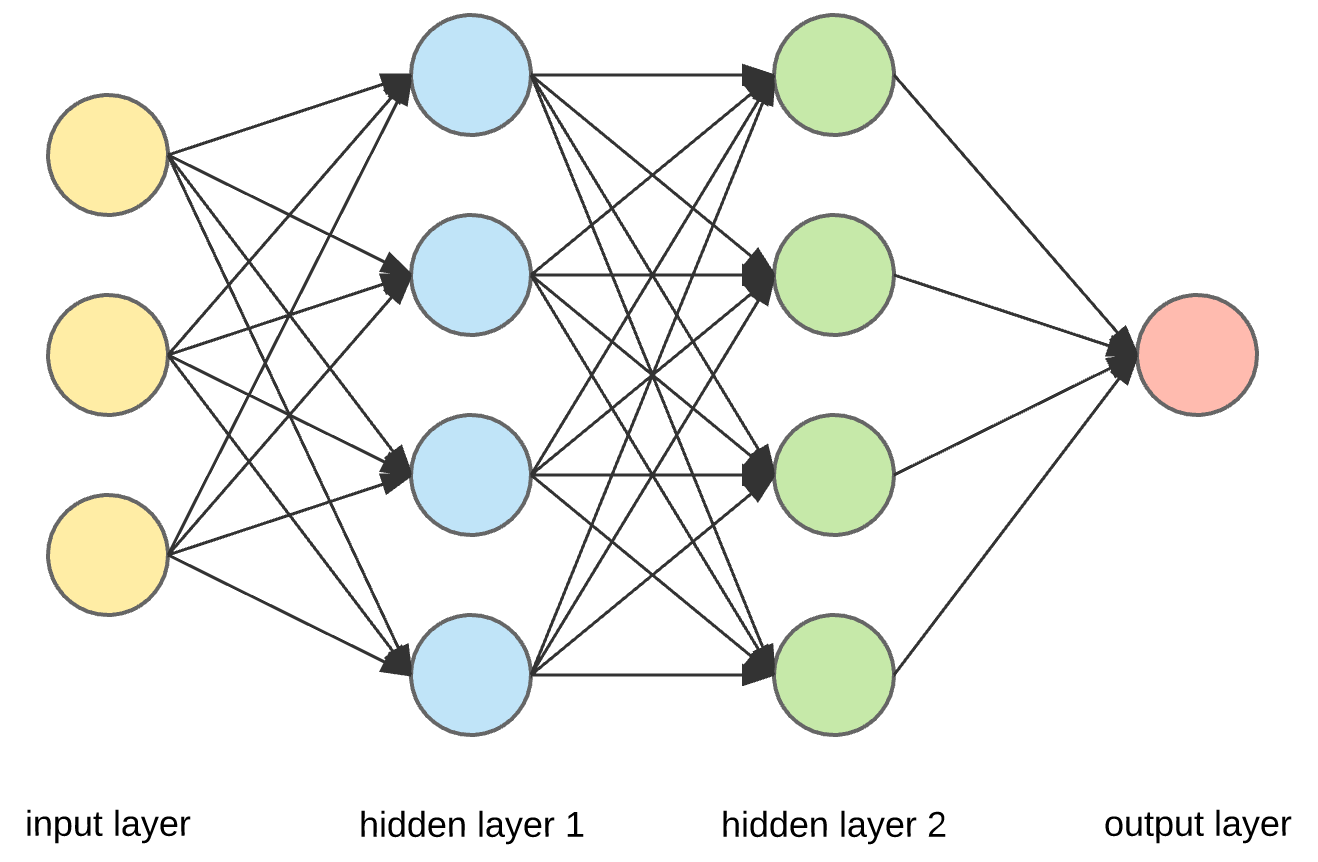
\includegraphics[width=0.4\linewidth]{figures/background/neural_network_architecture.png}
            \label{fig:neural_network_schema/feed-forward-architecture}
            }
        \hfill
        \subfloat[schematic drawing of a single neuron]{
            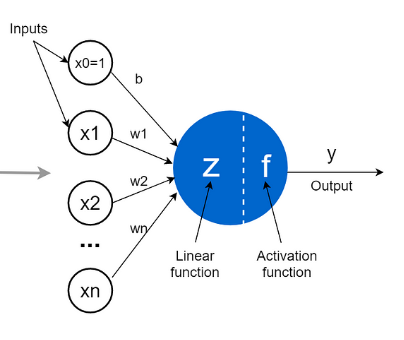
\includegraphics[width=0.4 \linewidth]{figures/background/neuron_schema.png}
            \label{fig:neural_network_schema/neuron}
            } 
    \end{center}
    \caption[neural network and neuron schema]{The figure shows the schematic drawing of a feed forward neural network and a neuron}
    \label{fig:neural_architecture}
\end{figure}

If we look at each individual neuron as in \figref{fig:neural_network_schema/neuron}, we can observe that each neuron is designed in the same way. First it calculates a weighted sum $z$ of its inputs $x$, the corresponding weights $w$ and bias $b$, before passing it into an activation function $h$ and finally passing the information to the next neuron. The activation function is designed to introduce nonlinearity into the model, allowing it to capture complex relationships between variables. Without a nonlinear activation function the whole network would be a single linear combination of its inputs and weights. Common activation functions include the sigmoid function, the hyperbolic tangent function, and the rectified linear unit (ReLU) function as in \figref{fig:activation_function}

\begin{figure}[t]
    \begin{center}
        \subfloat[Sigmoid]{
            
\includegraphics[width=0.3\linewidth]{figures/place_holder.png}
            \label{fig:activation_function/sigmoid}
            }
        \hfill
        \subfloat[hyperbolic tangent function]{
            
\includegraphics[width=0.3\linewidth]{figures/place_holder.png}
            \label{fig:activation_function/tanh}
            }
        \hfill
        \subfloat[rectified linear unit]{
            
\includegraphics[width=0.3\linewidth]{figures/place_holder.png}
            \label{fig:activation_function/relu}
            }
    \end{center}
    \caption[common activation functions in a neural network]{\textbf{common activation functions in a neural network}}
    \label{fig:action_function}
\end{figure}
\begin{figure}
    \begin{center}
        \subfloat[schematic drawing of convolutional neural network]{
            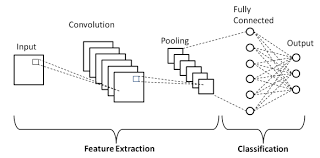
\includegraphics[width=0.4\linewidth]{figures/background/conv-net-architecture.png}
            \label{fig:neural-network-architecture/convolutional-architecture}
            }
        \hfill
        \subfloat[schematic drawing of a recurrent neural network]{
            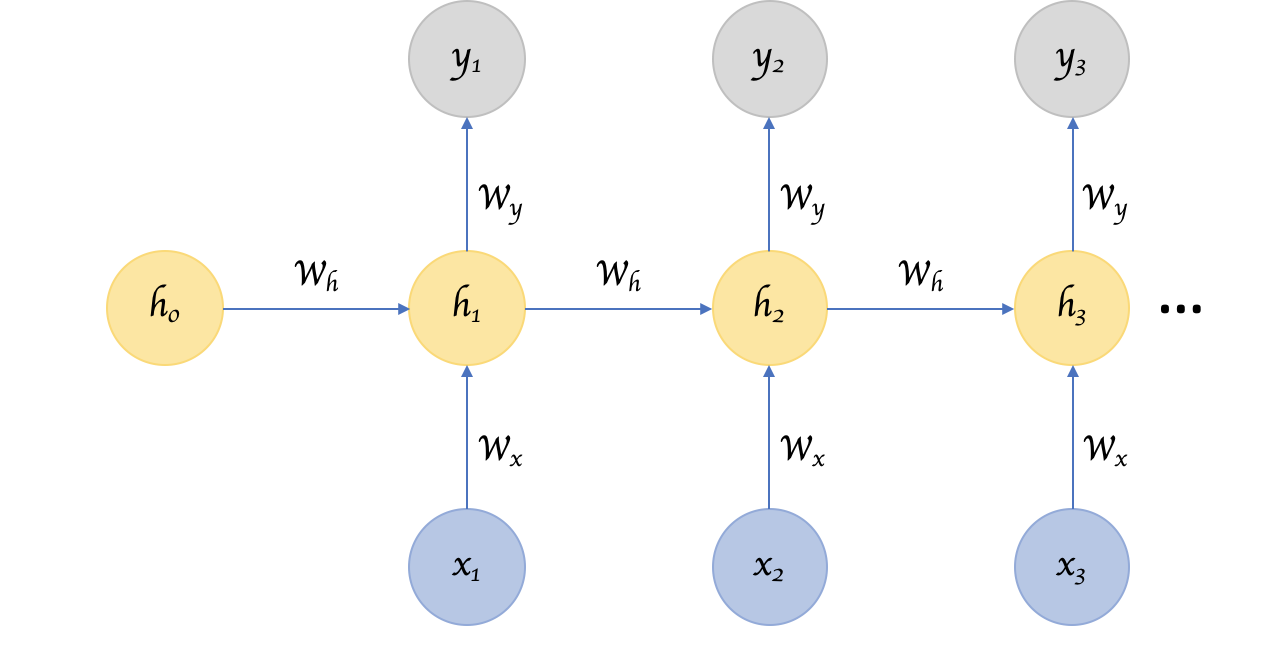
\includegraphics[width=0.4 \linewidth]{figures/background/rnn-net-architecture.png}
            \label{fig:neural-network-architecture/recurrent-architecture}
            } 
    \end{center}
    \caption[advanced neural network architectures]{architecture of more advanced neural networks like the convolutional and the recurrent neural network}
    \label{fig:neural_network-architecture}
\end{figure}

There are several types of neural network architectures but most of them are based on following types: 
\begin{itemize}
	\item \textbf{Feedforward networks} as in \figref{fig:neural_network_schema/feed-forward-architecture} are the simplest type of neural network, consisting of a series of layers that process information in a single direction.
	\item \textbf{Convolutional networks} as in \figref{fig:neural-network-architecture/convolutional-architecture} are designed for image processing tasks and use convolutional layers to identify patterns and features within images. 
	\item \textbf{Recurrent networks} as in \figref{fig:neural-network-architecture/recurrent-architecture}allow information to be passed between nodes in a cyclical manner, making them suitable for processing sequential data. The development of Long Short-Term Memory (LSTM) and Gated Recurrent Unit (GRU) architectures further improved RNNs' ability to model long-range dependencies.
\end{itemize}


\subsection{Train Neural Networks}

Neural networks are trained using techniques such as backpropagation and stochastic gradient descent as presented in \algoref{alg:SGD}. Backpropagation is an algorithm for calculating the gradient $\hat{g}$ of an optimization criterion with respect to the weights of the network. The gradient can then be used to update the weights and therefor improve the performance of the model with respect to the opimization function. A we can see in \algoref{alg:SGD} stochastic gradient descent minimizes the error presented by the opimization criterion by iteratively adjusting the weights based on randomly selected subsets of the training data. 

\begin{algorithm}
    \caption{Stochastic gradient descent}\label{alg:SGD}
    \begin{algorithmic}
        \State{} Input: Learning rate schedule: $\epsilon_1, \epsilon_2, \ldots$. Initial parameter $\theta$

        \State{} $k \leftarrow 1$
        \While{stopping criterion not met}
            \State{} Sample a minibatch of $m$ examples from training set $\{x^{(1)}, \ldots, x^{(m)}\}$ with corresponding targets $y^{(i)}$.
            \State{} Compute gradient estimate:
            \State{} $\hat{g} \leftarrow \frac{1}{m}\nabla_\theta \sum_i L(f(x^{(i)}; \theta), y^{(i)})$
            \State{} Apply update:
            \State{} $\theta \leftarrow \theta - \epsilon_k \hat{g}$
            \State{} $k \leftarrow k + 1$
        \EndWhile{}
\end{algorithmic}
\end{algorithm} 

Selecting a random subset of training data has a couple of advantages. 
\begin{itemize}
	\item \textbf{Computational Efficiency}: In one epoch we are computing the gradient only on a small subset. We do not have to pass the complete dataset through the network to get a sufficient gradient.
	\item \textbf{Improved Generalization}: Because each minibatch contains a different composition of data points from the dataset the gradient signal is also varying. These variations are improving the generalization of the model with respect to unseen data.
	\item \textbf{Avoiding Local Minima}: One of the risks during the training-process of a neural network are local minima. By introducing randomness through mini-batch sampling, SGD can escape local minima more easily and continue to explore the parameter space, increasing the chances of finding a global minimum.
	\item \textbf{Parallel Processing}: Using mini-batches allows parallel processing during training. 
\end{itemize}
\todo{find sources}



\subsection{Applications of Neural Networks}

% Provide examples of real-world applications of neural networks, such as natural language processing, computer vision, and autonomous vehicles
% Discuss the advantages and limitations of neural networks in different domains

Neural networks are widely used in real-world applications like in computer vision, marketing or medical applications. Particularly in combination with reinforcement learning they are successfully used in robotics for object recognition and manipulation, in gaming for complex decision-making, and in finance for predicting stock prices.

% \subsection{Current and Future Directions}
% 
% Describe current research trends in neural networks, such as transfer learning and % reinforcement learning
% Discuss potential future applications of neural networks, such as personalized medicine and % climate modeling
% Explain challenges that must be addressed in order for neural networks to continue to advance


\section{Variational Autoencoder}
% In this chapter we want to provide a intuition about Autoencoders 
% Based on the manifold hypothesis
% appoaches to solve this by principal component analysis
% Is a technique of unsupervised learning

Variational autoencoders (VAEs) and conditional variational autoencoders (CVAEs) are types of deep generative models that are used for unsupervised learning. Unsupervised learning is a type of machine learning where the model is not given labeled data for training. Instead, the model is tasked with finding patterns or structure in the data on its own. The goal of unsupervised learning is often to find hidden relationships or groupings within the data that can be used for further analysis or decision-making
VAEs and CVAEs are important because they can learn to generate realistic and diverse samples from complex high-dimensional data distributions, such as images or audio.

\subsection{Autoencoders}

% Describe traditional autoencoders and their limitations
% Explain how autoencoders can be used for unsupervised learning

Lets start with a Autoencoder. An Autoencoder $f = d \circ e$ consists of two parameterized function approximators in series, one encoder $e_\phi$ and one decoder $d_\psi$. 
The encoder maps the high dimensional input $x \in \mathbb{X}$ into a lower dimensional latent space $z \in \mathbb{Z}$, $z = e(x)$.
The latent vector $z$ is typically a lower dimensional representation of the input $x$. 
In the second stage we map the latent vector $z$ back into the high dimensional features space $X$, $d: \mathbb{Z} \to \mathbb{X}$. This should optimally reconstruct the given input $\hat{x} = d(z) = d(e(x))$. 

Because Autoenders are designed to learn a compact determin representation in the latent space it follows that similar input values $x$ should correspond to similar latent vectors $z$ and similar latent vectors $z$ correspond to similar outputs $\hat{x}$.

Traditional Autoenders have prooven to be successful on a variaty of task like: ..., but their simple and effective design comes along with some limitations:
\begin{itemize}
	\item Overfitting: Because of the deterministic mapping into the latent space and from the latent space back to the feature space traditional Autoencoders are prone to suffer from overfitting and can lack of regularization which could lead to poor performance on unseen data.
	\item Incomplete or noisy data: Due to the focus on only reconstructing the input, Autoencoders are not well suited for incomplete or noisy data. One reason could be the lack of disentanglement in the latent space, which means that different dimensions correspond to different underlying features in the input data distribution. 
	\item Probabilistic Interpretation: Another drawback of the deterministic mapping approach is the lack of probabilistic interpretation capabilities for uncertainty in the learned representation and generated outputs.  
\end{itemize}

\begin{figure}[t]
    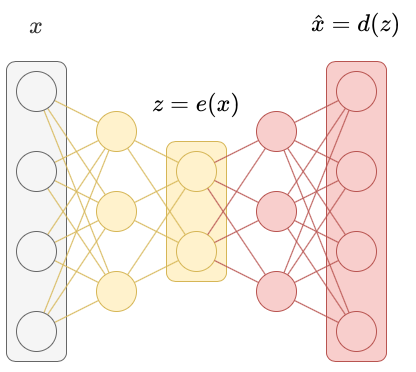
\includegraphics[width=0.5\linewidth]{figures/background/AE.png}
    \caption[Autoencoder schematics]{\textbf{schematic drawing of a Autoencoder}}
    \label{fig:Autoencoder_schematics}
\end{figure}

\subsection{Variational Autoencoders}\label{sec:VAE}

\todo{ELBO: https://probml.github.io/pml-book/book2.html 779}

A Variational Autoencoder is similar to an Autoencoder but also with some key changes. Similar are the basic setup as a generative unsupervised learning model and the underlying encoder decoder structure. The key difference lays in the in the latent space between the encoder and decoder. Instead of having a fixed deterministic latent space VAEs operate on a probabilistic latent space.

\begin{figure}
    \centering
    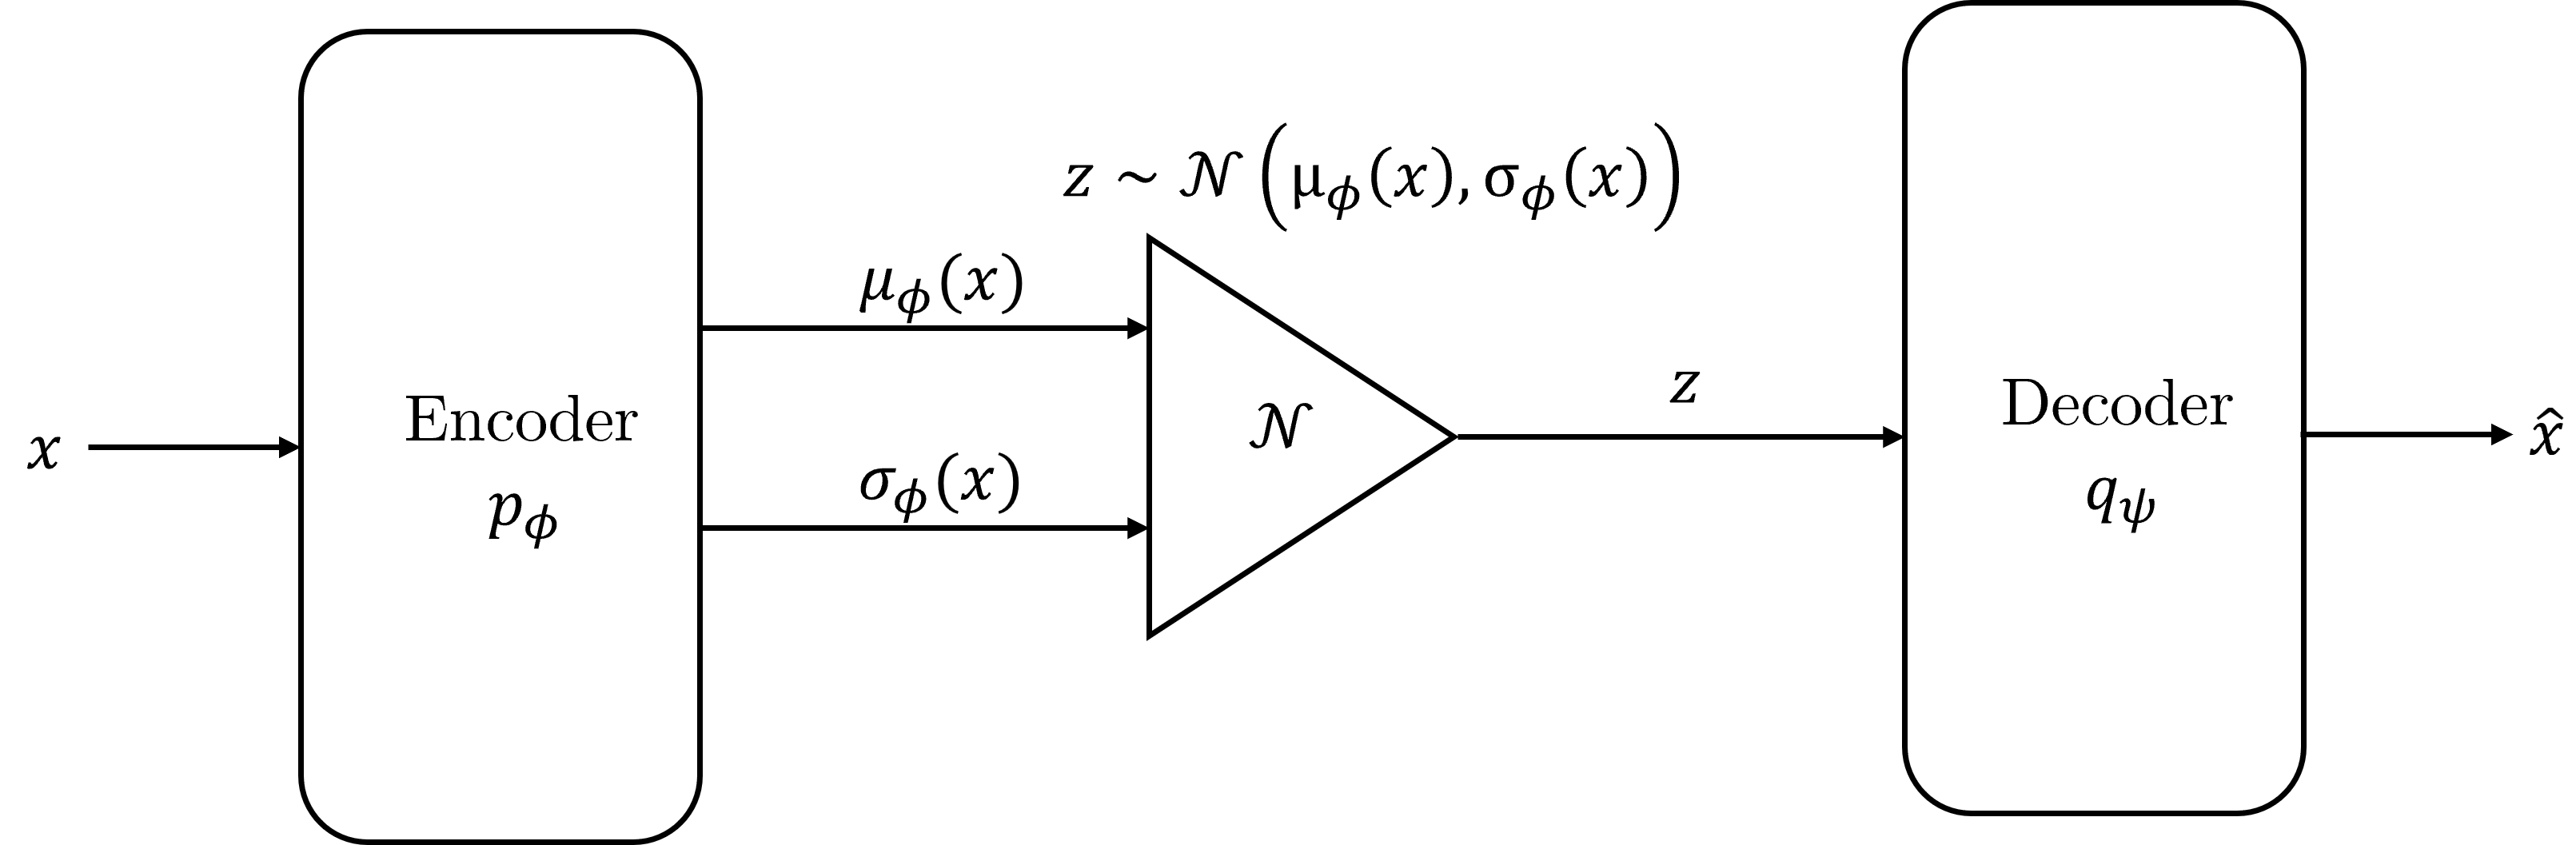
\includegraphics[width=0.5\linewidth]{figures/background/VAE.png}
    \caption[Variational Autoencoder schematics]{\textbf{schematic drawing of a Variational Autoencoder}}
    \label{fig:Variational_Autoencoder_schematics}
\end{figure}

The encoder network denoted as a approximated parameterized posterior distribution $q_\phi(z|x)$, is a conditional probability distribution in Bayesian inference with the probability of the latent variable $p(z)$ (the prior) and the evidence $p(x)$: 

\begin{align}
	q(z|x) &= \frac{p(x|z) p(z)}{p(x)} \label{eqn:Bayesian-inference}\\
	p(x) &= \int p(x|z)p(z) dz \label{eqn:p(x)}
\end{align}

In the context of a Variational Autoencoder, calculating $q(z|x)$ is not possible. As we can see in \eqref{eqn:p(x)} accessing the evidence as the probability of the observed data is not possible because we have to integrate over all possible values of the latent variable $z$. Therefor we approximate the posterior distribution with a parameterized conditional distribution $q_\phi(z|x)$. $q_\phi(z|x)$ as known as the encoder network, parameterized with $\phi$, hereby maps input data $x$ to latent parameters like mean and variance for a gaussian distribution, of the latent distribution with random variable $z$. 

On the other hand, the decoder network takes samples from the latent space with latent variables $z$ and reconstructs the data from these samples, generating a parameterized probabilistic distribution over the data given the latent variables $p_\psi(x|z)$. 

As mentioned before the objective in training a Variational Autoencoder is to find parameters $\phi$ and $\psi$ and matches best the true posterior distribution. In order to do so we can use the Evidence Lower Bound as the objective function. We go a bit deeper into the fundamentals of the Evidence Lower bound in \secref{sec:ELBO}. \\
During training, the VAE aims to maximize the ELBO by iteratively adjusting its parameters $\phi$ and$\psi$ using backpropagation. The encoder network maps the input data to a distribution over latent variables, while the decoder network reconstructs the data from the sampled latent variables. The reparameterization trick similar to SAC in \secref{sec:SAC} is employed to ensure differentiability during backpropagation through the stochastic sampling process. \todo{reparaphrase}


% Explain the concept of a latent variable and how it relates to VAEs
% Describe the architecture of a VAE and how it differs from a traditional autoencoder
% Explain how the encoder and decoder are trained using a variational inference approach
% Describe the role of the Kullback-Leibler (KL) divergence in the loss function

\subsection{Conditional Variational Autoencoders}

\begin{figure}
    \begin{center}
        
\includegraphics[width=0.5\linewidth]{figures/place_holder.png}
        \caption[Conditional Variational Autoencoder schematics]{\textbf{schematic drawing of a conditional Variational Autoencoder}}
        \label{fig:conditional-Variational_Autoencoder_schematics}
    \end{center}
\end{figure}
% Describe the architecture of a CVAE and how it differs from a VAE
% Explain how CVAEs can be used for supervised learning tasks
% Describe the role of the conditional input in the encoder and decoder
A Conditional Variational Autoencoder is an extension of the VAE architecture that takes into account conditional information $c$. As we can see in \figref{fig:conditional-Variational_Autoencoder_schematics}In a Conditional Variational Autoencoder, both the encoder and decoder are modified to accept an additional input that represents the conditional information. 

The role of the conditional input in the encoder is to help the model capture the conditional dependencies between the input data and the class label. So the conditional information could be for instance a label encoding or a set of labels that describe the class or category to which the input belongs. The encoder must learn to map both the input data and the conditional input to a meaningful latent space representation that captures the relevant information for the generation process. In the decoder, the conditional input is used to guide the generation process and ensure that the generated samples are representative of the specified class.

Similar to Variational Autoencoders the objective function to train the encoder and decoder is the Evidence Lower Bound. But there have to be a couple of changes to make the individual ELBO components suitable to take the conditional information $c$. The final objective can be observed in \eqref{eqn:ELBO-CVAE}. 


\subsection{Evidence Lower Bound}\label{sec:ELBO}

The Evidence Lower Bound (ELBO) is a fundamental concept in the training of Variational Autoencoders (VAEs)
It is derived from the principle of variational inference and represents a lower bound on the log-likelihood of the data given the model's parameters. Maximizing the ELBO is equivalent to minimizing the Kullback-Leibler (KL) divergence between the true posterior distribution $q(z|x)$ over latent variables $z$ and the approximated posterior distribution $q_\phi(z|x)$ used in the VAE.

\begin{equation}\label{eqn:ELBO}
	L_\text{ELBO}(x, z) = \mathbb{E}_{z\sim q_\phi(\cdot|x)} \left[ \log p\psi(x|z) \right] - \text{KL}\left( q_\phi(z|x) \| p(z) \right)
\end{equation}

Further I will discuss the individual components of the Evidence lower bound 
\begin{itemize}
	\item \textbf{Posterior Distribution}: In general the posterior distribution $q(z|x)$ is considered as the probability of the latent variable $z$ given the observed data $x$. Specific for Variational Autoencoder it can be computed from Bayesian Inference as in \eqref{eqn:Bayesian-inference} which is as mentioned in \secref{sec:VAE} not feasible is therefor approximated.
	\item \textbf{Likelihood}: The likelihood function $p(x|z)$ or conditional likelihood in the context of probabilistic models is the probability distribution of the observed data $x$ given the latent variables $z$. Dependent on the observed data it is possible to chose from a set of different probability distributions. Examples are a multivariate gaussian distribution for continuous data, a Bernoulli distribution for binary data or categorical distribution for discrete data with multiple categories.
	\item \textbf{Prior Distribution}: The prior distribution $p(z)$ is a probabilistic distribution that represents the initial belief or assumption about the latent variables $z$ in Bayesian inference. Additional $p(z)$ serves in Variational Autoencoder as a regularizer during training as it encourages the VAE to learn meaningful and smooth latent representations in the latent space. Most popular choice for the prior distribution is the standard normal distribution $\mathcal(N)(0, I)$.  
	\item \textbf{Evidence}: p(x) represents the evidence, also known as the marginal likelihood or model evidence, in the context of Bayesian statistics. It is the probability of the observed data $x$ given a particular statistical model. The evidence serves in \eqref{eqn:p(x)} as a normalization constant, ensuring that the posterior distribution $q(z|x)$ over model parameters integrates to 1. It quantifies how well the model, with its specific set of parameters, explains or fits the observed data.
	\item \textbf{Reconstrion Loss}: 
	\begin{equation}\label{eqn:general-reconstruction-loss}
		\mathbb{E}_{z\sim q(\cdot|x)} \left[ \log p(x|z) \right] \approx \mathbb{E}_{z\sim q_\phi(\cdot|x)} \left[ \log p_\psi(x|z) \right]
	\end{equation}
	Therm (\ref{eqn:general-reconstruction-loss}) measures the similarity between the reconstructed data and the original input. 
	Described in words it is the expected log-likelihood of the data given the latent variables, which is computed by sampling from the approximating distribution $q_\phi(z|x)$ and evaluating the likelihood $p_\psi(x|z)$ using the decoder network.
	\item \textbf{KL Divergence Loss}: 
	\begin{equation}
		\text{KL}\left( q(z|x) \| p(z) \right) \approx \text{KL}\left( q_\phi(z|x) \| p(z) \right)
	\end{equation}
	This term quantifies the difference between the approximated parameterized posterior distribution $q_\psi(z|x) $ over latent variables $z$ and a chosen prior distribution $p(z)$. As mentioned before it is a popular choice to use a standard normal distribution $p(z)=\mathcal(N)(0,I)$ as the prior distribution. The KL divergence encourages the latent variables to be close to the prior distribution, promoting regularization and preventing overfitting.
\end{itemize}

\todo{Explain prior and posterior distributions}
\iffalse
The posterior distribution, denoted as q(z|x), is a conditional probability distribution in Bayesian inference. In the context of Variational Autoencoders (VAEs), the posterior distribution refers to the distribution of the latent variables z given the observed data x.
In VAEs, the encoder network parameterizes the approximate posterior distribution q(z|x), which takes the input data x as input and outputs the parameters (e.g., mean and variance) of the distribution over the latent variables z. The encoder learns to map the data x to a distribution in the latent space, where each point in the latent space represents a potential encoding of the data.
The posterior distribution q(z|x) is essential in the VAE framework because it allows the model to learn meaningful and compressed representations of the input data. By optimizing the ELBO (Evidence Lower Bound), VAEs simultaneously maximize the likelihood term (the data reconstruction term) and minimize the KL divergence term, encouraging the approximate posterior to be close to the prior distribution p(z).
The posterior distribution q(z|x) plays a central role in VAEs, enabling the model to capture the underlying structure of the data and support various applications, such as data generation and latent space interpolation.

The prior distribution, denoted as p(z), is a probabilistic distribution that represents our initial belief or assumption about the latent variables z in Bayesian inference. In the context of Variational Autoencoders (VAEs), the prior distribution refers to the distribution of the latent variables z before observing any data.
In VAEs, the prior distribution is typically chosen to be a simple and well-known distribution, such as a standard normal distribution with zero mean and unit variance, i.e., p(z) = N(0, 1). Using a standard normal distribution as the prior is a common choice due to its simplicity and ease of sampling.
The prior distribution serves as a regularizer during training and plays a crucial role in VAEs' generative process. By incorporating the prior distribution in the ELBO (Evidence Lower Bound) objective function, VAEs are encouraged to learn meaningful and smooth latent representations. The KL divergence term in the ELBO measures the difference between the approximate posterior distribution q(z|x) (learned by the encoder) and the prior distribution p(z). Minimizing this term ensures that the approximate posterior is close to the prior distribution, promoting regularization and preventing overfitting.
The choice of the prior distribution can impact the VAE's performance and the characteristics of the generated data. While a standard normal distribution is commonly used, VAEs can be adapted to use other types of priors, such as uniform distributions or more complex distributions, depending on the specific requirements of the application.
\fi

The basic notation of the Evidence Lower Bound for Variational Autoencoders as in \eqref{eqn:ELBO} can be easily extented for an Conditional Variational Autoencoder:
\begin{equation}\label{eqn:ELBO-CVAE}
	L_\text{ELBO}(x, z, c) = \mathbb{E}_{z\sim q_\phi(\cdot|x, c)} \left[ \log p\psi(x|z, c) \right] - \text{KL}\left( q_\phi(z|x, c) \| p(z|c) \right)
\end{equation}
\todo{Describe also the components of the CVAE ELBO }


By optimizing the ELBO, VAEs effectively learn to approximate the true posterior distribution and generate meaningful latent representations of the data, enabling various tasks such as data generation, interpolation, and denoising within a Bayesian framework.

\subsection{VAEs and CVAEs in Practice}

% Provide examples of real-world applications of VAEs and CVAEs, such as image and text generation, and conditional image generation
% Explain how VAEs and CVAEs can be used for data compression and denoising
% Describe the advantages and limitations of VAEs and CVAEs compared to other % generative models

VAEs and CVAEs have been successfully applied to a wide range of real-world applications. In image generation, VAEs have been used to generate novel images of faces, objects, and scenes. Similarly, CVAEs have been used for conditional image generation, allowing for the generation of images based on specific attributes or classes. In text generation, VAEs have been used to generate natural language sentences and paragraphs.

VAEs and CVAEs can also be used for data compression and denoising. By learning a compressed representation of the input data, VAEs and CVAEs can reduce the dimensionality of the input space while preserving important features. Similarly, by learning to reconstruct the original input from noisy or corrupted data, VAEs and CVAEs can be used for denoising and data restoration.

One of the advantages of VAEs and CVAEs is their ability to learn a continuous latent representation of the input data. This allows for easy manipulation and exploration of the latent space, enabling applications such as image editing and style transfer \todo{cite paper}.

However, VAEs and CVAEs have some limitations. The generated samples may not be as sharp or detailed as those produced by other generative models such as GANs \todo{cite}. Additionally, the trade-off between the reconstruction loss and the KL divergence term can be difficult to balance, potentially leading to overfitting or underfitting \todo{paper}. Nonetheless, VAEs and CVAEs remain a popular and powerful tool for generative modeling and data compression.


% \subsection{Extensions to VAEs and CVAEs}
% 
% Describe extensions to the basic VAE and CVAE architectures, such as hierarchical VAEs and semi- supervised VAEs
% Explain how VAEs and CVAEs can be combined with other models, such as Generative Adversarial % Networks (GANs)

% \subsection{Current and Future Directions}
% 
% Describe current research trends in VAEs and CVAEs, such as improving the quality of generated samples and addressing the mode collapse problem
% Discuss potential future applications of VAEs and CVAEs, such as in healthcare and climate modeling
% Explain challenges that must be addressed in order for VAEs and CVAEs to continue to advance

% \subsection{Conclusion}
% 
% Summarize the main points of the chapter
% Emphasize the importance of VAEs and CVAEs in a variety of fields
% Encourage further exploration of the topic.

\section{Kinematics}

Kinematics is the study of motion, specifically the description and analysis of the position, velocity, and acceleration of objects or systems without considering the forces causing the motion. It focuses on understanding the spatial relationships and geometrical aspects of moving objects. The following sections provide an insight into forward and inverse kinematics for kinematic chains. Those two concepts are often used in robotics, animation, virtual reality or even protein folding. 

\subsection{Forward kinematics}

Forward kinematics is a concept from robotics that involves determining the position and orientation of an end-effector, like a gripper of a robot arm, based on the joint angles and geometric parameters, like segment length, of the system. It provides a mathematical model for mapping the joint angles to the end-effector position in order to understand the overall configuration and motion of the robot. \eqref{alg:FK} describes a forward kinematics implementation. 

\begin{algorithm}
    \caption{Forward Kinematics}\label{alg:FK}
    \begin{algorithmic}
        \State{} Input: Current joint angles $q$, Segment Length $l$.
        \State{} Define origin position in 2D space: $p \leftarrow (0, 0)$
        \For{each $i$ in $[0, \ldots, N - 1]$}
            \State{} Update position
            \State{} $p_0 \leftarrow p_0 + \cos(q_i) * l_i$
            \State{} $p_1 \leftarrow p_1 + \sin(q_i) * l_i$
        \EndFor{}
\end{algorithmic}
\end{algorithm}

Throughout this thesis this function is used with a constant segment length $l = \{1\}^N$ therefor it is referred to as in \eqref{eqn:FK} which maps an angle configuration $q$ into the end-effector position in 2D space.

\begin{equation}[p]\label{eqn:FK}
	fk: \mathbb{R}^N \to \mathbb{R}^2
\end{equation}

\subsection{Inverse kinematics}

Inverse kinematics (IK) is a fundamental problem in robotics, animation or virtual reality that involves finding a required joint angle configuration or positions to reach a desired end-effector position and optionally a desired orientation. It plays a crucial role in controlling the motion and manipulation of robotic systems, enabling them to interact with the environment and perform complex tasks. 
In this section you will find a brief summary of existing approaches, a deeper explanation of the Cyclic Coordinate Descent algorithm and the description of the used inverse kinematics RL environment.

\subsubsection{Existing Approaches to Solve Inverse Kinematics}

Numerous approaches have been proposed to solve the inverse kinematics problem. These approaches can be broadly categorized into: 
\begin{itemize}
	\item analytical methods: rely on geometric methods to derive closed form solutions.
	\item numerical methods: iteratively approximate the joint angles that satisfy the desired end-effector position and orientation.
	\item heuristic methods: iteratively propagate positions along the kinematic chain to converge on the desired end-effector position.
	\item sampling-based methods: randomized search strategy to explore the joint space and find feasible solutions to the inverse kinematics problem
\end{itemize}

% \subsubsection{Existing Approaches to Solve Inverse Kinematics Extended}

% \textbf{Analytical Methods}: Some robotic systems with simple geometries and kinematic structures can be solved analytically using closed-form solutions. Analytical methods often rely on geometric techniques and mathematical equations such as the Denavit-Hartenberg (DH) parameters to derive explicit formulas for the joint angles. These methods provide fast and exact solutions when applicable, but they are limited to specific cases with well-defined geometric relationships.

% \textbf{Numerical Methods}: Numerical methods for inverse kinematics aim to iteratively approximate the joint angles that satisfy the desired end-effector position and orientation. Jacobian-based methods, such as the Jacobian transpose method and the Jacobian pseudo-inverse method, leverage the Jacobian matrix to relate the end-effector velocities to the joint velocities. These methods iteratively adjust the joint angles based on the discrepancy between the actual and desired end-effector positions. Other numerical techniques, including cyclic coordinate descent, Gauss-Newton, Levenberg-Marquardt, and optimization algorithms like Particle Swarm Optimization and Genetic Algorithms, aim to find optimal joint configurations by minimizing an objective function that represents the error between the desired and actual end-effector positions.

% \textbf{Heuristic Methods}: Heuristic methods, such as the Forward and Backward Reaching Inverse Kinematics (FABRIK) algorithm, iteratively propagate positions along the kinematic chain to converge on the desired end-effector position. These methods provide an intuitive and efficient way to solve inverse kinematics problems and handle complex robotic structures with multiple degrees of freedom.

% \textbf{Sampling-Based Methods}: Sampling-based methods, such as Randomized Kinodynamic Planning (RRT), adopt a randomized search strategy to explore the joint space and find feasible solutions to the inverse kinematics problem. By sampling and connecting valid configurations in the joint space, these methods can discover feasible joint angles that satisfy the end-effector constraints.

% \textbf{Machine Learning-based Methods}: Machine learning approaches, including neural networks and reinforcement learning algorithms, have been increasingly explored for solving inverse kinematics. Neural networks can be trained to approximate the inverse kinematics mapping based on input-output data pairs. Reinforcement learning algorithms, such as Soft Actor-Critic (SAC), can learn inverse kinematics policies through trial-and-error interactions with the environment, optimizing joint configurations to achieve desired end-effector positions.

\subsubsection{Cyclic Coordinate Descent}

Cyclic Coordinate Descent (CCD) is a popular numerical method for solving inverse kinematics. It is an iterative algorithm that adjusts the joint angles of a robotic system one at a time, from a base joint to the end-effector, in order to align the end-effector with the desired target position.

The algorithm works by iteratively updating the joint angles based on the discrepancy between the current and desired end-effector positions ($p_\text{target}$). At each iteration, CCD focuses on a single joint and adjusts its angle to minimize the positional error. By sequentially updating the joint angles in a cyclic manner, CCD aims to converge towards a solution that satisfies the desired end-effector position.

\begin{algorithm}
    \caption{Cyclic Coordinate Descent Pseudo Code}\label{alg:CCD}
    \begin{algorithmic}
        \State{} Input: Current joint angles $q$, Desired end-effector position $p_\text{target}$.
        \While{unitl convergence}
            \For{each $i$ in $[N-1, \ldots, 0]$}
                \State{} Calculate the vector from the current joint position to the end-effector position:
                \State{} $V_\text{current} \leftarrow p_{N-1} - p_i$

                \State{} Calculate the vector from the current joint position to the target position:
                \State{} $v_\text{target} \leftarrow p_\text{target} - p_i$

                \State{} Calculate the rotation necessary to align $v_\text{current}$ with $v_\text{target}$:
                \State{} $\delta q_i \leftarrow \text{angle\textunderscore between}(v_\text{current}, v_\text{target})$

                \State{} Update the joint angel:
                \State{} $q_i \leftarrow q_i + \delta q_i$
            \EndFor{}
        \EndWhile{}
\end{algorithmic}
\end{algorithm}

As illustrated in \algoref{alg:CCD} and \figref{fig:background/CCD geometry} in each iteration, CCD calculates the vector from the current joint position $p_i$ with $p_i$ as the position of the $i$th joint with $i \in \{0, \ldots, N-1\}$, to the end-effector position ($v_\text{current}$) and the vector from the current joint position to the target position ($v_\text{target}$). By finding the rotation necessary to align $v_\text{current}$ with $v_\text{target}$, represented as $\delta\phi$, the algorithm updates the joint angle accordingly. This process is repeated for each joint in the kinematic chain until convergence is achieved.

\begin{figure}[ht]
	\centering
	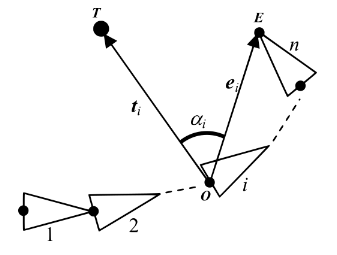
\includegraphics[width=0.9\textwidth,]{figures/background/CCD-geometry.png}
	\caption{CCD geometry}
	\label{fig:background/CCD geometry}
\end{figure}
\todo{make own figure}

\todo{experiments for runtime analysis in dependence of number of joints}

    \chapter{Methodology}\label{chap:Methodology}

In this section, we are going to explain the research idea and introduce the inverse kinematics benchmark environment. Further, we will dive a bit deeper into the techniques to create a dataset and explain the used criteria for the latent models. We are going to conclude this chapter by providing a short introduction to the software written and used tools.

\section{Research Idea}

The primary research idea of this thesis is to pursue a transformation from the RL environment action space $\mathcal{A}$ into a lower-dimensional latent action space $\mathcal{A}_L$. This latent action space will align with the latent space between the encoder and decoder of a VAE model or the feature space of a feed-forward neural network. By doing so, we aim to enable RL agents to effectively explore and learn within a more compact and smoothened action representation. A schematic drawing can be revisited at \figref{fig:research_idea}

We propose two potential approaches for achieving this dimensionality reduction: VAEs and supervised models.

In the VAE approach, a conditional or unconditional generative model is employed to learn a latent representation of the action space. By training the VAE on actions from an expert or on state target combinations to emphasize a solution that is independent of an expert, we aim to capture the underlying structure and patterns within the action space from the RL environment. This latent representation can potentially offer a more concise and informative representation of the actions, and encourage more efficient learning and exploration for RL agents.

Alternatively, the supervised model approach involves training a supervised learning model, such as a neural network, to directly transform the defined lower-dimensional latent action into the high-dimensional action space. This transformation is learned based on labeled examples of actions and their corresponding latent representations. In the conducted experiments the lower dimensional-action space is just the desired action outcome. By leveraging supervised learning techniques, we aim to find a mapping between state information and desired action outcome to the RL environment action space, allowing the RL agent to operate effectively on a higher level within the reduced-dimensional latent action space.
\begin{figure}
    \centering
    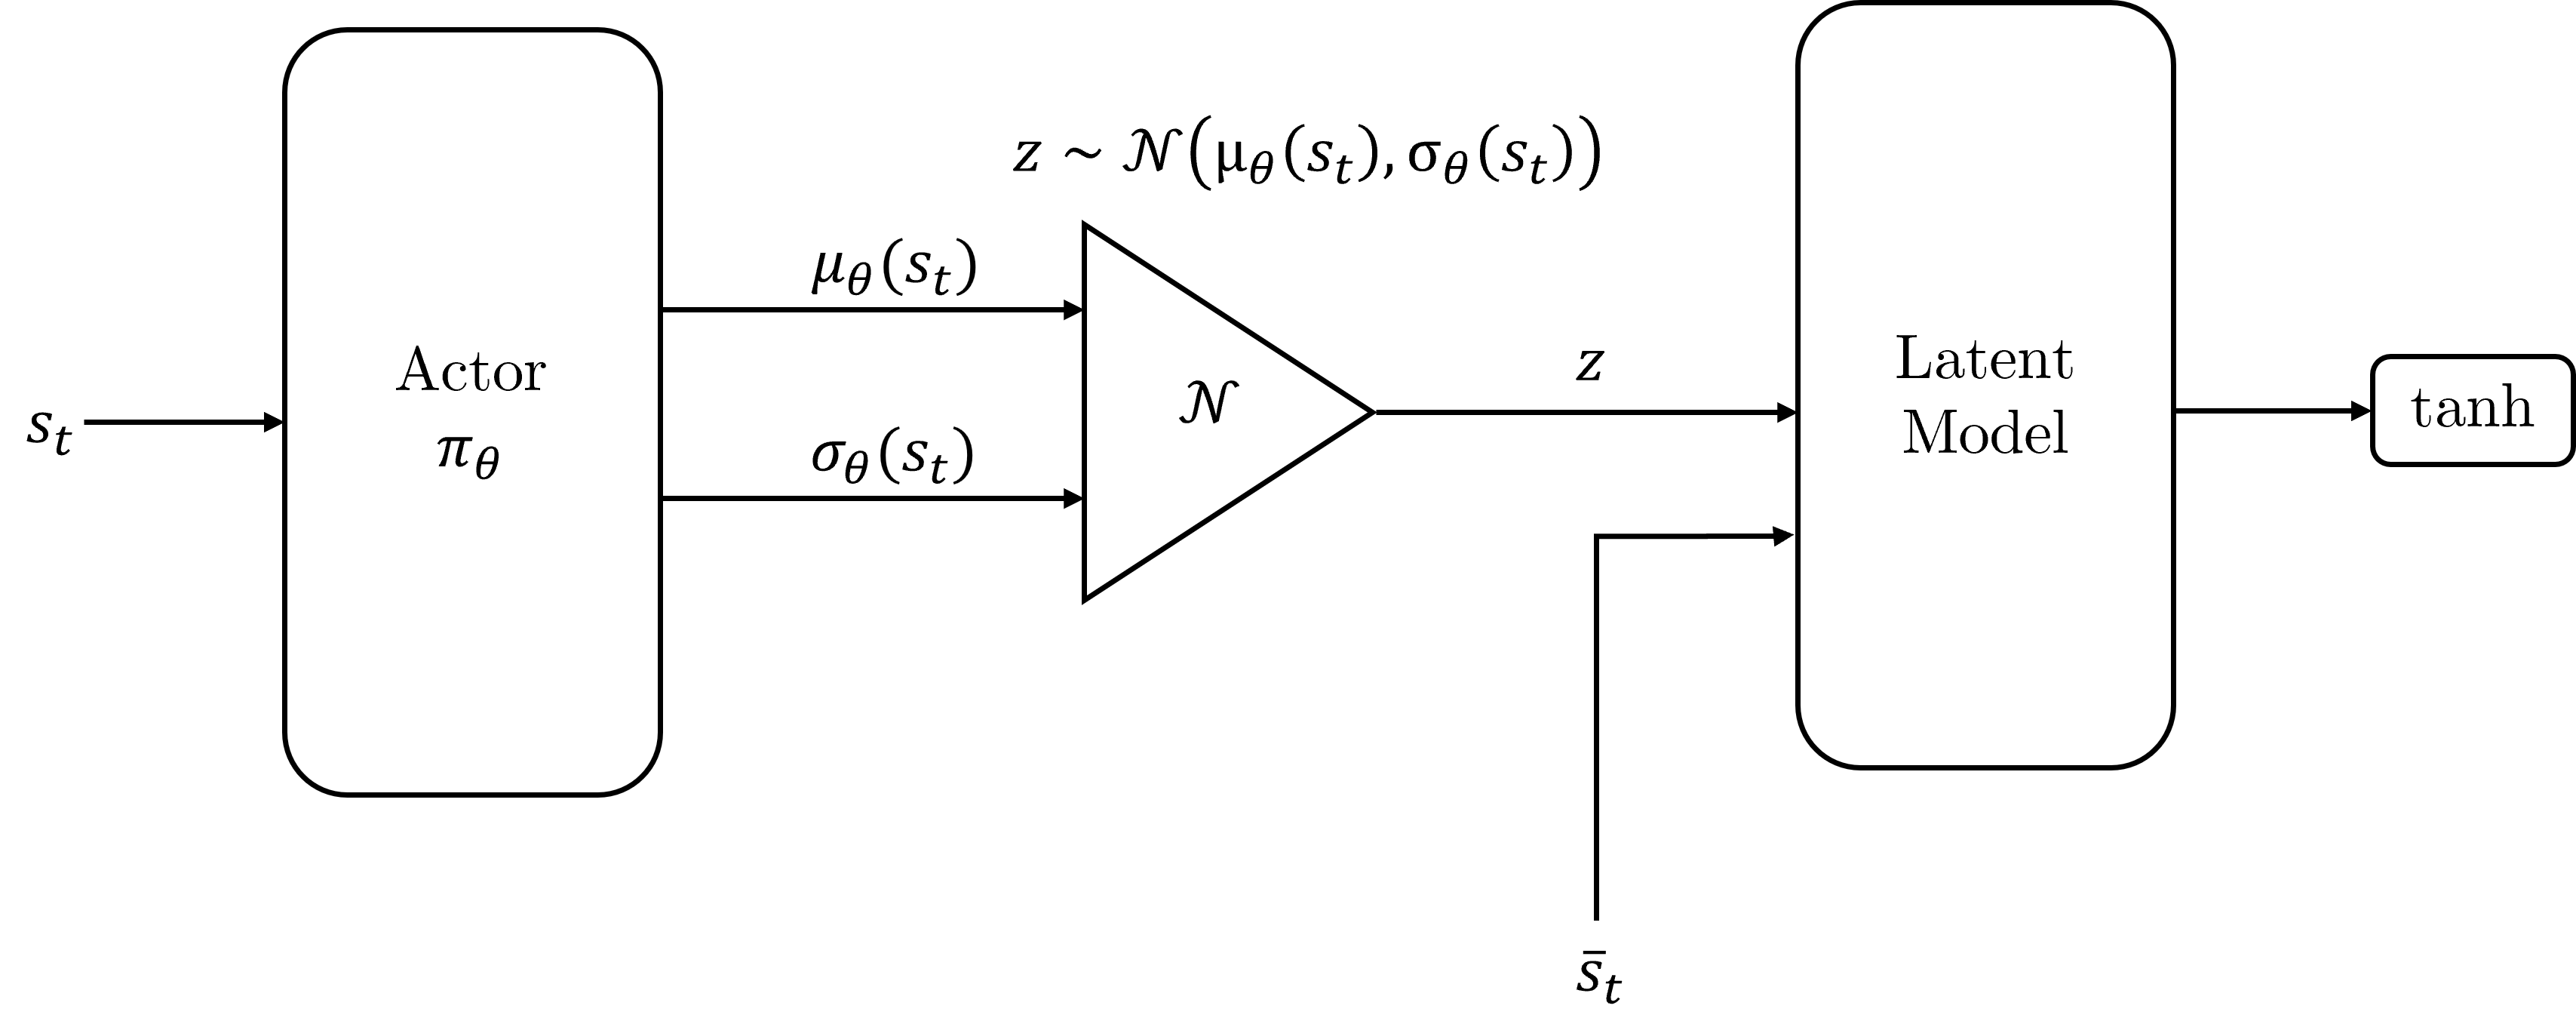
\includegraphics[width=0.7\textwidth,]{figures/methodology/SAC+LatentModel.png}
    \caption[Research idea]{Schematic drawing of how the models would be chained together. The latent model will be replaced by either the decoder of a VAE, a CVAE, or a supervised feed-forward network. Note that we adapt the additional information $\bar{s_t}$ by the needs of the individual models. }
    \label{fig:research_idea}
\end{figure}

\section{RL Environment}\label{sec:RL-Environment}

To apply RL in general you need an environment the agent can send actions to and receive feedback as discussed in \secref{sec: RL-Framework}. As previously introduced the key problem we are targeting is inverse kinematics of a robot arm. This problem turns out to be suitable because:
\begin{itemize}
    \item the action space is scalable by simply adding additional joints to the robot arm
    \item it can be simplified into a 2D space with a fast and reliable implementation
    \item it is expandable. You are always able to extend the environment with additional constraints like objects the robot has to navigate around or joint angle constraints.
\end{itemize}

In this section, we are going to present a novel RL-Environment for bench-marking the performance of different algorithms to solve inverse kinematics for a robot arm with $N$ many joints and subsequently $N$ many segments with lengths $l \in\mathbb{R}_{>0}^N$ in 2D space. For simplicity reasons $l$ is constant with $l = \{1\}^N$ as a vector with length $N$ and filled with ones. The environment is embedded into the Farama Gymnasium framework~\cite{Gymnasium}.

\begin{figure}[h]
    \centering
    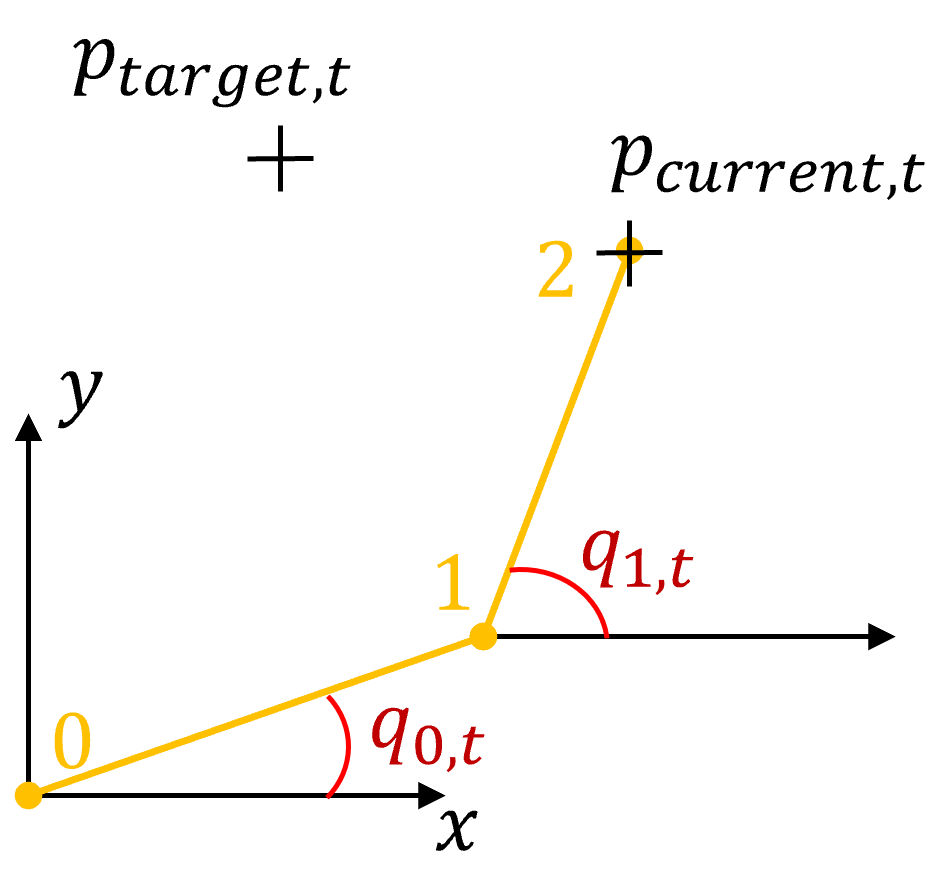
\includegraphics[width=0.4\textwidth,]{figures/methodology/EnvExample.png}
    \caption[Plane Robot Environment]{Schematic drawing of the individual state space components.}
    \label{fig:plane_robot_env}
\end{figure}

\subsection{State Space}

The state space $\mathcal{S} \subset \mathbb{R}^{4 + N}$ for this environment consists of three main building blocks. 

\begin{itemize}
    \item \textbf{goal information} $p_{\text{target}, t} \in \mathbb{R}^2$: This vector provides information where to move the end-effector. This position lies in for the robot arm, reachable distance. Mathematical speaking: $||p_\text{target}||_2 \leq \sum_{i = 1}^N l_i$ 
    \item \textbf{state position} $p_{\text{current},t} \in \mathbb{R}^2$: This vector contains the current end-effector position in 2D space and should help the agent to understand where the end-effector is placed and how an action has influenced the current end-effector position. Because the current position is attached to the robot arm: $||p_\text{current}||_2 \leq \sum l$.
    \item \textbf{joint angles} $q_t \in [0, 2\pi^N)$: This vector contains information about the joint angle configuration at time $t$. Note that each joint angle describes the delta angle between the joint direction and a horizontal line from the origin in the positive x direction.
\end{itemize}
A state $s_t \in \mathcal{S}$ at time $t$ has for all $t$ the same composition

\begin{equation}\label{eqn:state}
    s_t = (p_{\text{target}, t}, p_{\text{current}, t}, q_t)
\end{equation}

To refer to individual parts from index $i$ to $j$ of a state with $s_{t, (i, j)}$. Therefore we can extract the individual parts with:
\begin{itemize}
    \item $p_{\text{target}, t} = s_{t, (0, 1)}$ 
    \item $p_{\text{current}, t} = s_{t, (2, 3)}$
    \item $q_{t} = s_{t, (4, N + 4)}$
\end{itemize}

\subsection{Action Space}

The action space $\mathcal{A} \subseteq \mathbb{R}^N$ for this particular environment is continuous and contains all possible joint angle configurations for a robot arm with $N$ joints. 

A generated action $\hat{a}$ from the agent is sent to the environment. Inside the environment, the incoming action is added on top of the current state angles $q_t$. To ensure the constraints of $q_{t+1} \in [0, 2\pi)^N$ we take the signed remainder of a division by $2\pi$ to write into $q_{t+1}$:
\begin{equation*}
    q_{t+1} = (q_t + \hat{a}) \ \% \ 2\pi
\end{equation*}

Subsequently after updating the state angles the current end-effector position gets updated by a forward kinematics call on $q_{t+1}$:
\begin{equation*}
    p_{\text{current}, t} = \text{FK}(q_{t+1})
\end{equation*}


\subsection{Reward Function}

The reward function $R: \mathcal{A} \times \mathcal{S} \to \mathbb{R}$ as in~\eqref{eqn:Rewardfunction} for the conducted experiments and this environment aims to minimize the distance between the current end-effector position $p_{\text{current}, t}$ and the current target position $p_{\text{target}, t}$. The current end-effector position is calculated by the forward-kinematics function on state angles $q_t$ plus action $a_t$. The target position is sampled at the beginning of an episode and stays constant throughout the episode until completion or a time limit is reached. 

\begin{equation}\label{eqn:Rewardfunction}
    R(s_t, a_t) = - ||FK(s_{t, (4, \ldots, N + 4)}  + a_t) - s_{t, (0 ,1)}||_2
\end{equation}

If you want to normalize the reward function you have to divide $R$ by $N$.

\begin{figure}[h]
    \centering
    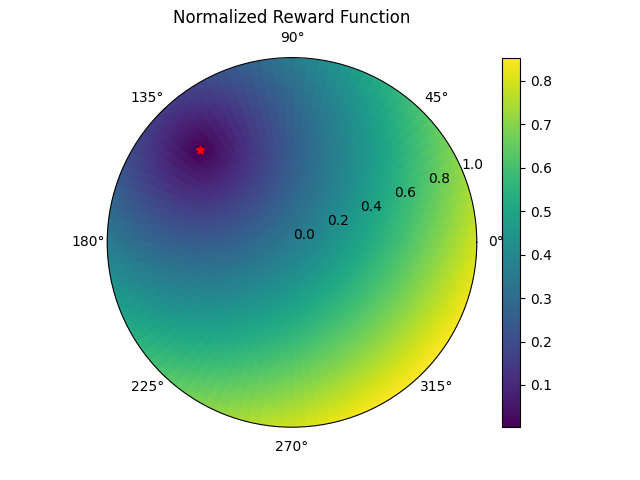
\includegraphics[width=0.5\textwidth,]{figures/methodology/RewardFunction.png}
    \caption[Reward function]{Normalized Reward function with $q \in [0, 2\pi]^N$ as element of the whole space and $p_\text{target} = [-0.5, 0.5]$. The target position $p_\text{target}$ is marked with a red star.}
    \label{fig:Reward_function}
\end{figure}

In \figref{eqn:Rewardfunction} we can see the linear gradient for any current position towards the target position at $[-0.5, 0.5]$.

\section{Dataset Creation}\label{sec:Dataset_creation}

To realize the idea of joining a latent model to the actor-network of SAC we do need a dataset to train such a latent model. A dataset should contain environment state information as well as possible actions.
Consistent over all experiments with the VAE and Supervised Model sizes of the datasets are consistent:
\begin{itemize}
    \item train: 10.000 data points
    \item validation: 2000 data points
    \item test: 1000 data points
\end{itemize}

\subsection{Uniform Sampling} \label{sec:vanilla_sampling}

The vanilla sampling algorithm for sampling a dataset is to sample state angles $q_t$ and actions $a_t$ from a uniform distribution

\begin{equation} \label{eqn:angle_sample}
    q_t, a_t \sim \mathcal{U}_{[0, 2\pi)}^N
\end{equation}

and the target position with

\begin{align}
    p &= [\cos(\beta), \sin(\beta)] \cdot r \label{eqn:position_sample}\\
    \beta &\sim \mathcal{U}_{[0, 2\pi)} \ \ r \sim \mathcal{U}_{[0, N]} \nonumber
\end{align}

While observing $p_{\text{current}, t}$ in \figref{fig:Uniform_dataset/scatter} we can observe that with an increasing number of joints, the scattered dots are forming a two-dimensional Gaussian distribution around the origin. As we can see in \figref{fig:Uniform_dataset/std} the standard deviation is exponentially decreasing. 
\begin{figure}
    \begin{center}
        \subfloat[Scatter plot of different end effector positions generated by applying forward kinematics on uniformly sampled angles. The end effector positions are normalized by their corresponding number of joints. This leads to the constraint that all positions have a maximum distance to the origin of 1. For each number of joints, we sample $5\mathrm{e}{3}$ angles. The upper and right plots describe the density function of an end-effector position.]{
            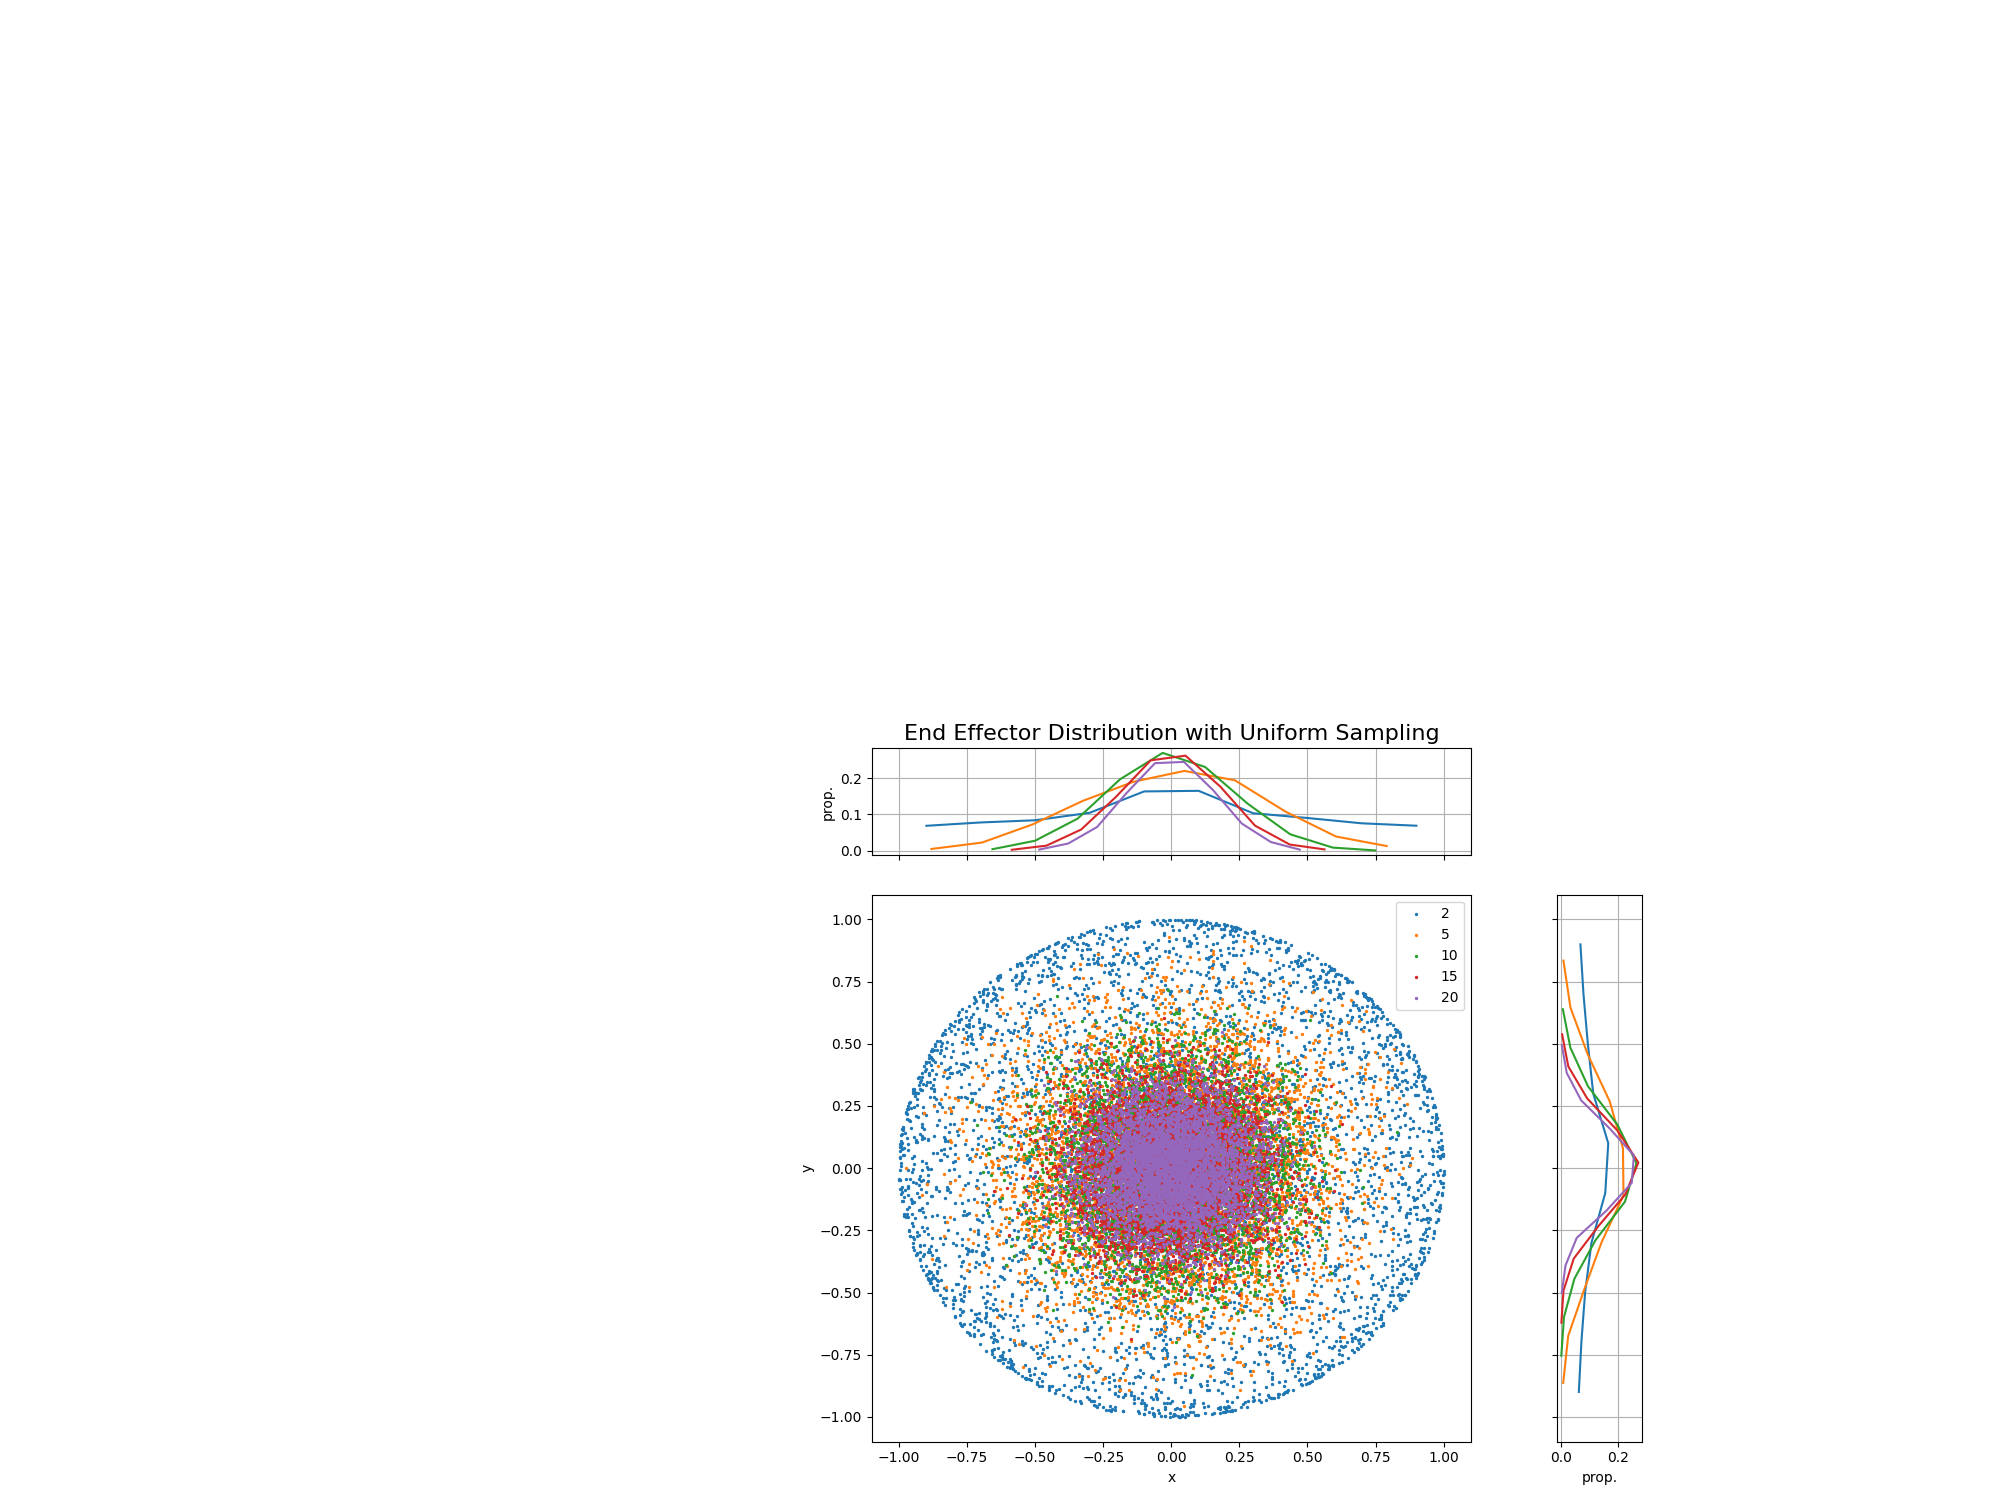
\includegraphics[trim={18cm 0 5cm 3cm}, width=0.46 \linewidth]{figures/methodology/relative_end_effector_scatter.png}\label{fig:Uniform_dataset/scatter}}
        \hfill
        \subfloat[Standard deviation of end effector positions in x and y direction concerning the number of joints for a robot arm. For each number of joints, we sample $1\mathrm{e}{4}$ angles. ]{
        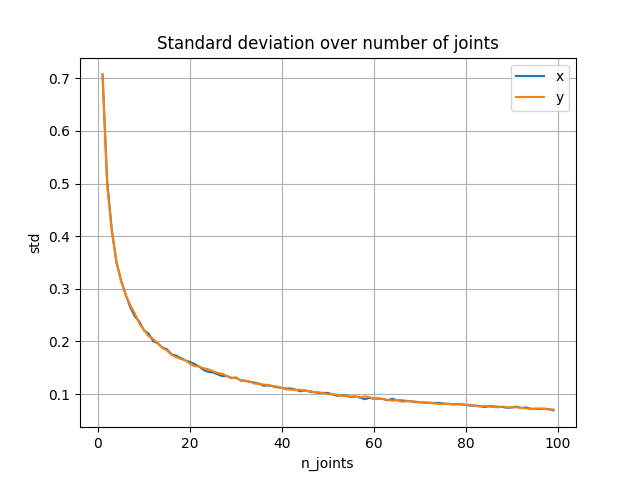
\includegraphics[width=0.46 \linewidth]{figures/methodology/std_over_n_joints.png}\label{fig:Uniform_dataset/std}}
    \end{center}
    \caption[Uniform dataset properties]{Properties of the dataset with actions sampled from a uniform distribution. }\label{fig:Uniform_dataset}
\end{figure}

In our application, this makes the vanilla algorithm not suitable because we are not covering the observation space close to the maximum reach of the robot arm with more than 2 joints. 

\subsection{Expert Guidance}

The problems encountered with the vanilla sampling algorithm in \secref{sec:vanilla_sampling} lead to the development of a separate sampling algorithm that involves guidance by an expert. 

\begin{algorithm}
    \caption{Expert Guided Dataset Creation}\label{alg:Expert_Dataset}
    \begin{algorithmic}
        \State{} Input: number of joints: $N$, number of samples: $K$.
        \State{} $\mathcal{D} \leftarrow \{\}$  Dataset
        \For{$i \in [0, \ldots, N -1]$}
            \State{} $p_{\text{current}} \leftarrow (\text{\ref{eqn:position_sample}})$ sample a position in 2D space with~\eqref{eqn:position_sample}
            \State{} $q_t \sim \mathcal{U}$ sample initial arm angles from a uniform distribution as in~\eqref{eqn:angle_sample}
            \State{} $q_t \leftarrow IK(q_t, p_{\text{current}})$ solve IK for $p_{\text{current}}$ and with $q_t$ as start
            \State{} $p_{\text{target}} \leftarrow (\text{\ref{eqn:position_sample}})$ sample a position in 2D space with~\eqref{eqn:position_sample}
            \State{} $a_t \leftarrow IK(q_t, p_{\text{target}}) - q_t$ IK for the target position
            \State{} $\mathcal{D}_i \leftarrow ((p_{\text{target}}, p_{\text{current}}, q_t), a_t)$
        \EndFor{}
\end{algorithmic}
\end{algorithm}
The clear advantage of this algorithm is that we ensure now that $p_{\text{target}}$ and $p_{\text{current}}$ are uniform concerning direction and distance to the origin.

On the other hand, we are now bound to the actions the $IK$-solver, in our application CCD as in \algoref{alg:CCD}, is providing. This could lead to unpredicted behavior of the RL agent if we leaf the covered part of $q_t$ as shown in \figref{fig:dataset_action_correlation}. Another disadvantage is that this algorithm is now much slower compared to the vanilla sampling algorithm. 
\begin{figure}
    \begin{center}
        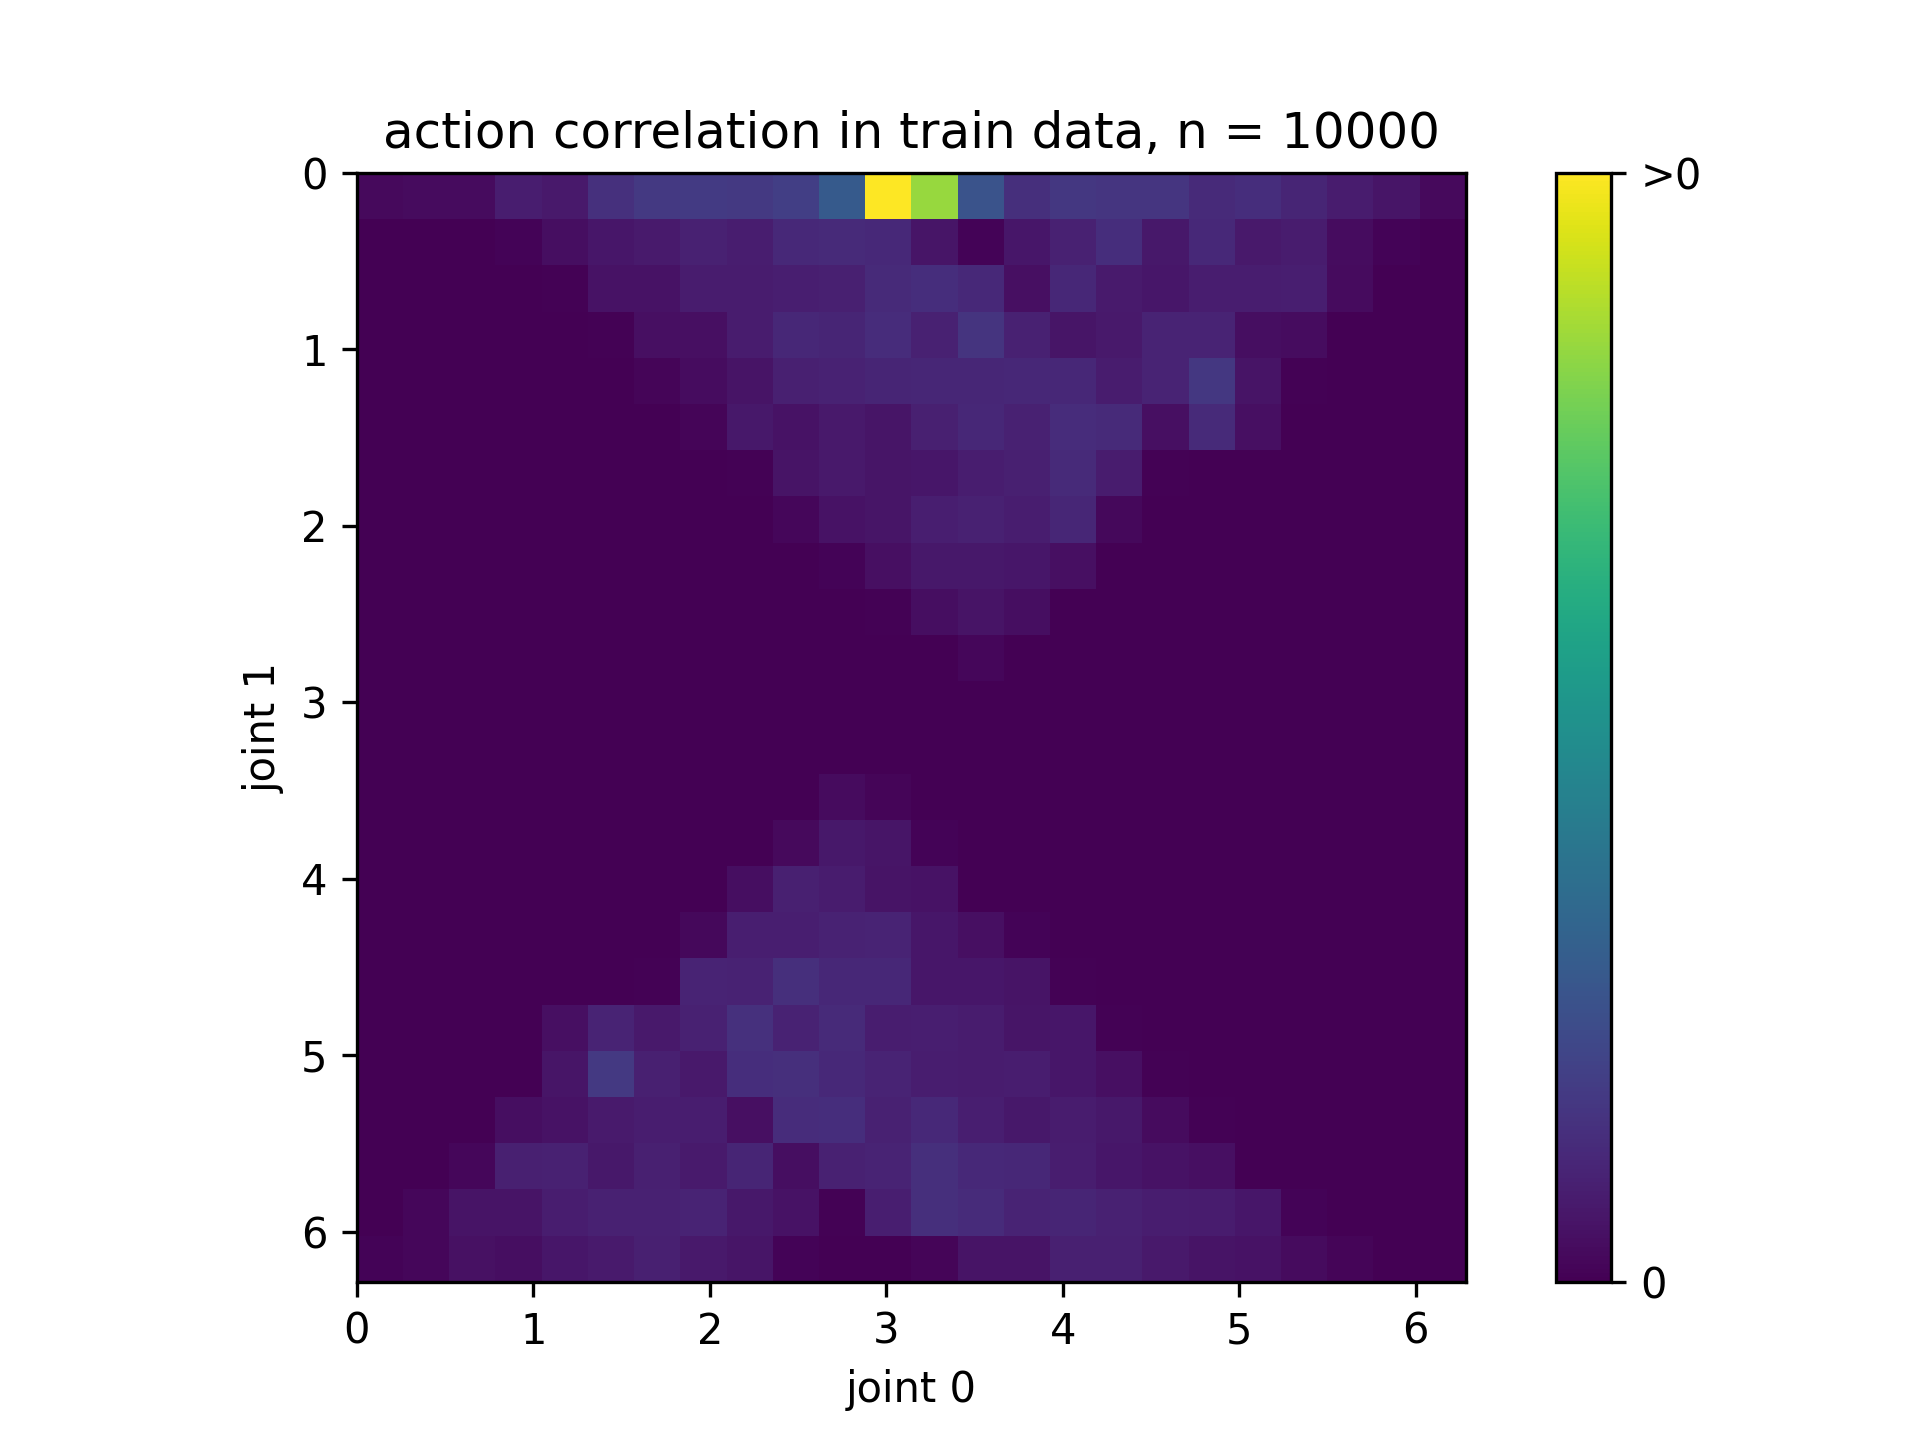
\includegraphics[width=0.46 \linewidth]{figures/methodology/dataset/action_correlation.png}
    \end{center}
    \caption[action correlation CCD]{Plotted is the state angle correlation of two joints as a 2D histogram. Each bucket can be translated to the number of angles in one 3D bucket $b$ with limits $b_{0, 0}, b_{0, 1}, b_{1, 0}, b_{1, 1}$. Mathematical speaking: $|b| = |\{q_t | q_t \in [0, 2\pi)^2 \land q_{0, t} \in [b_{0, 0}, b_{0, 1}] \land q_{1, t} \in [b_{1, 0}, b_{1, 1}]\}|$}
    \label{fig:dataset_action_correlation}
\end{figure}

To have a more detailed look into the runtime complexity we focus on the runtime complexity of CCD as this is the slowest part of \algoref{alg:Expert_Dataset}. We can observe that the runtime of each CCD run is different since CCD belongs to the family of iterative inverse kinematics solvers and the runtime is either limited by a given maximum number of iterations or a break condition depending on how close we are to the goal. \\
In \figref{fig:expert_dataset/runtime_histograms} we can see that all probability density functions have a similar shape but with different means. Since we are interested in the runtime complexity of CCD we plotted the mean runtime of each density function in \figref{fig:expert_dataset/runtime_complexity}. Here we can observe that the runtime complexity of CCD is at least $\mathcal{O}(N^k)$ with $k \geq 3$ since the first-order empirical derivation is still at least quadratic. Further derivations would be not plausible because with each derivation we would decrease the number of data points by one and therefore have no points left anymore.
\begin{figure}
    \begin{center}
        \subfloat[continuous density function of collected runtimes of CCD over a different amount of joints. For each joint, we sampled 1000 different start conditions, (target, angles) for CCD to solve inverse kinematics. Note that the x-axis is in the log scale. ]{
            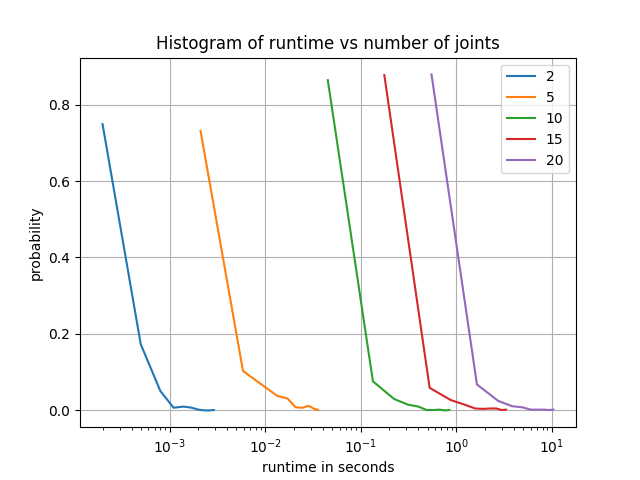
\includegraphics[width=0.46 \linewidth]{figures/methodology/dataset/runtime_histograms.png}
            \label{fig:expert_dataset/runtime_histograms}
            }
        \hfill
        \subfloat[plotted is the mean runtime for 1000 runs of CCD over the number of joints]{
        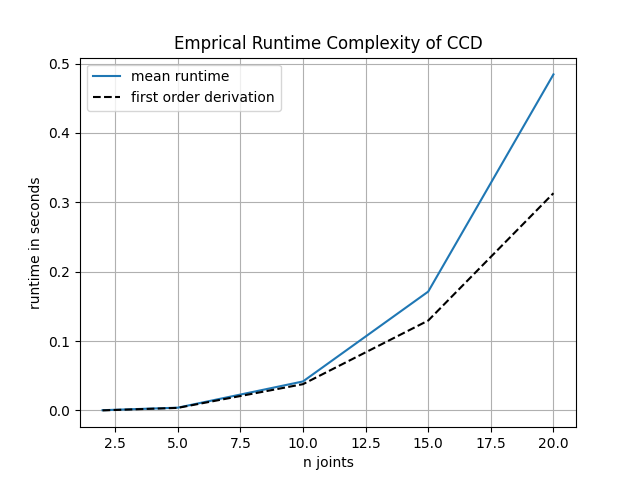
\includegraphics[width=0.46 \linewidth]{figures/methodology/dataset/runtime_complexity.png}
            \label{fig:expert_dataset/runtime_complexity}
            }
    \end{center}
    \caption[Runtime complexity CCD]{Runtime complexity CCD}
    \label{fig:expert_dataset}
\end{figure}

Another interesting point of view is the correlation between resulting angles from CCD. Since we are limited to a maximal two-dimensional plot we can only plot a heatmap to show the correlations between state joint actions as in \figref{fig:dataset_action_correlation}. Important to note that the actions are already in environment format and therefore are absolute angles concerning a horizontal line in the positive x direction. We can clearly see that CCD does not use the whole space but only focuses on a rhombus-shaped area. 

\section{Latent Criterion}


In this section, we will cover the employed loss functions to train the latent models. 
As discussed in \secref{sec:VAE} we employ the Evidence Lower Bound as the objective function to train Variational Autoencoder. To fit our problem of inverse kinematics we tried out 3 different reconstruction loss functions.

In this section, we will explain the tangible KL divergence as well as the individual reconstruction loss functions.

\subsection{Kulback Leiber Divergence}

The Kulllback Leiber divergence first published by Solomon Kullback and Richard Leiber in 1951~\cite{pml2Book} is a mathematical measure of how a probability distribution $P$ differs from a second distribution $P'$ and is denoted as $D_\text{KL}(P||P')$. Inside the ELBO it functions as a regularization element between the latent distribution $p_\phi(z|x)$ and a target distribution $p(z)$. Throughout this thesis, we take the standard normal distribution as the target distribution, $p(z) = \mathcal{N}(0, I)$. Since we implement a parameterized Gaussian as the latent distribution due to the nature of continuous input data, $p_\phi(z|x) = \mathcal{N}_\phi(\mu_\phi(x)| \ \Sigma_\phi(x))$. Therefore we can calculate the Kullback Leiber Divergence as:
\begin{align*}
    D_\text{KL}( \mathcal{N}_\phi(\mu_\phi(x)| \Sigma_\phi(x))|| \mathcal{N}(0, I)) &= \frac{1}{2} \left(\mu_\phi(x)^T\mu_\phi(x)  + tr\left(\Sigma_\phi(x)\right) - K - \log{|\Sigma_\phi(x)|} \right)\\
    &= \frac{1}{2} \left(\mu_\phi(x)^T\mu_\phi(x)  + \sum_{i=1}^K\Sigma_\phi(x)_{ii} - K - \log\left(\sum_{i=1}^K\Sigma_\phi(x)_{ii}\right)\right) 
\end{align*}

\subsection{Reconstruction Loss}

Inside the Evidence Lower Bound objective, the reconstruction loss minimizes the distance between the input data $x$ and the model output $\hat{x}$. In our experiments, we employed three different approaches for the reconstruction loss:

\textbf{Imitation Loss}. The imitation loss is a criterion to minimize the mean squared error between a given label $y$, in this case, an action from an expert which results in $y \in \mathbb{R}^N$ and the predicted action $\hat{x} \in \mathbb{R}^N$. It is defined as in~\eqref{eqn:Imitation-Loss}.

\begin{equation}\label{eqn:Imitation-Loss}
    \begin{split}
        \mathcal{L}_\text{Imi}: \mathbb{R}^N \times \mathbb{R}^N & \to \mathbb{R} \\
        y, \hat{x} & \mapsto \frac{1}{N}\sum_{i = 0}^{N-1} \left(y_i - \hat{x}_i\right)^2 
    \end{split}
\end{equation}

\textbf{Distance Loss}. This loss function minimizes the distance between a desired position in 2D space as label $p_\text{target}$ and the action outcome of a state action combination. The state information needed for this criterion is only the current robot arm angles $q$. Like before the action is referred to as $\hat{x}$.

\begin{equation}\label{eqn:Distance-Loss}
    \begin{split}
        \mathcal{L}_\text{Dist}: \mathbb{R}^2 \times \mathbb{R}^2 \times \mathbb{R}^N & \to \mathbb{R} \\
        p_\text{target}, \hat{x}, q & \mapsto ||p_\text{target} - \text{FK}(q + \hat{x})||_2
    \end{split}
\end{equation}

This criterion is also used in a standard supervised learning approach where the model predicts actions based on state information.

\textbf{Inverse kinematics Loss}. This criterion as in~\eqref{eqn:IK-Loss} is the result of merging distance loss and imitation loss in one loss function as a weighted sum of those two components with weights $w_\text{Imi}, w_\text{Dist} \in \mathbb{R}$. Inside the code, the loss function can also be configured to work also a pure distance loss function without providing any expert action and make it therefore also applicable to the aforementioned supervised learning approach. 

\begin{equation}\label{eqn:IK-Loss}
    \begin{split}
        \mathcal{L}_\text{IK}: \mathbb{R}^2 \times \mathbb{R}^2 \times \mathbb{R}^N, \mathbb{R}^N & \to \mathbb{R} \\
        p_\text{target}, \hat{x}, q, y  &\mapsto w_\text{Imi} \cdot \mathcal{L}_\text{Imi}(y, \hat{x}) + w_\text{Dist} \cdot \mathcal{L}_\text{Dist}(p_\text{target}, \hat{x}, q)
    \end{split}
\end{equation}

\section{Learning the Latent Model}

For the upcoming experiments, we settled on one setting with one kind of dataset, the Target Gaussian. \\
The idea behind the Gaussian target dataset is to learn an action that moves the end-effector towards a target sampled from a two-dimensional Gaussian distribution around the end-effector as demonstrated in \figref{fig:TargetGaussian_Schematics}.
\begin{figure}
    \begin{center}
        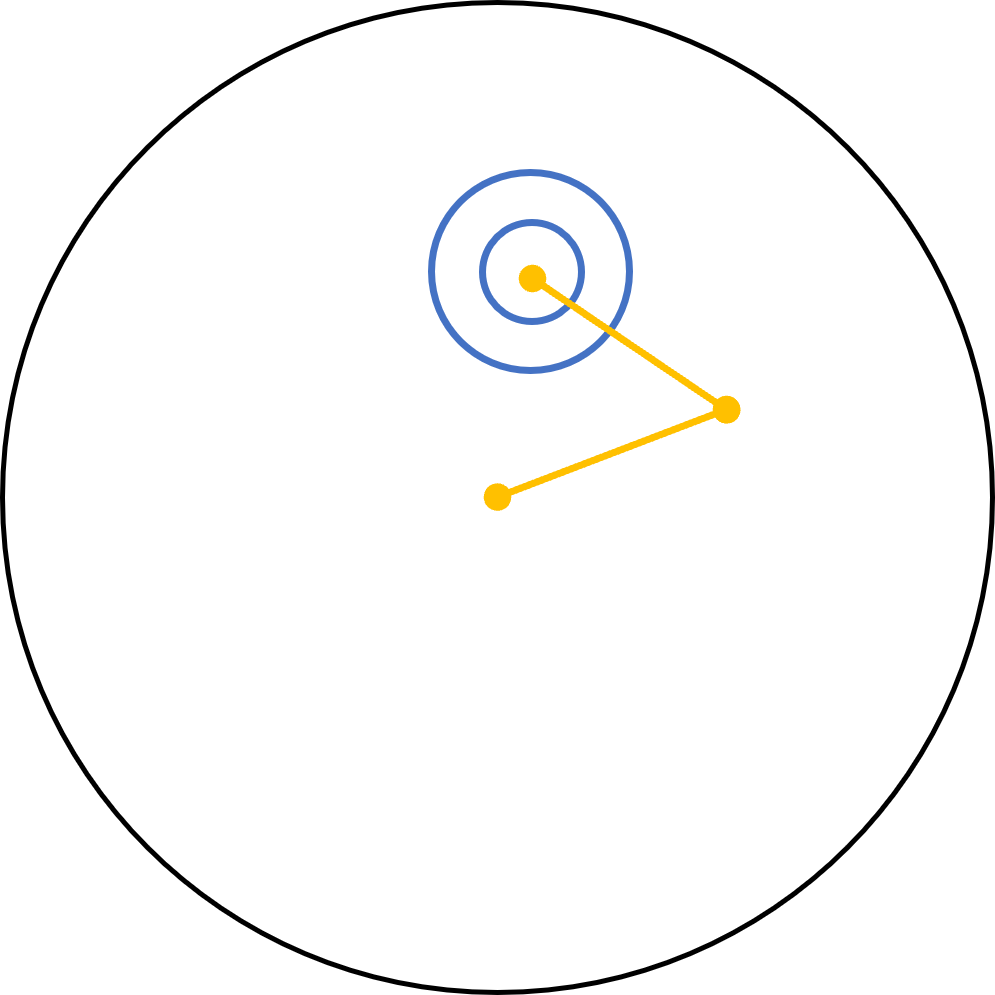
\includegraphics[width=0.3 \linewidth]{figures/experiments/VAE/TargetGaussian.png}
    \end{center}
    \caption[Target Gaussian Schematics]{Schematic drawing of how the target Gaussian dataset works. First, we are going to take the state as it comes from \algoref{alg:Expert_Dataset} (in yellow). Then we are going to sample a target position from inside a two-dimensional truncated or nontruncated Gaussian distribution (in blue) and define it as a new target position. Optionally we can also compute the corresponding CCD action.}\label{fig:TargetGaussian_Schematics}
\end{figure}

\begin{table}[]
    \centering
    \begin{tabular}{l|l}
        Name & Value \\
        \hline
        VAE $x$ & $p_{\text{target}, t}$ \\
        Supervised $x$ & $s_t$ \\
        $c$ & $(p_{\text{current}, t}, q_t)$ \\
        $\hat{x}$ & $q_{t + 1}$
    \end{tabular}
    \caption[Latent workflow parameter]{Latent workflow parameter with their correlation}
    \label{tab:Latent Parameter}
\end{table}

While training the Variational Autoencoder we settled on hyperparameter as described in \chapref{chap:appendix} and input vectors as in \tabref{tab:Latent Parameter}. It is important to note that $x$ for VAE, concatenated with $c$ equal to $s_t$ which is the same input as for the Supervised model. 

While training VAE and Supervised model you have to account for the additional hyperbolic tangent function in the back of \figref{fig:research_idea}. This additional stage is introduced with an instance of \texttt{PosProcessor}. The \texttt{PosProcessor} is enabled during training the latent model but deactivated during training SAC because SAC applies a hyperbolic tangent function in the \texttt{PolicyNet}. 

\section{Software}

In this section, we present the software stack developed to train the latent models and the reinforcement learning agent for our research. The software tools are available on the following GitHub repositories:

\begin{itemize}
    \item Latent Models and RL Agent: \url{https://github.com/RobinU434/Bachelorthesis}
    \item Inverse Kinematics Environment: \url{https://github.com/RobinU434/IK-RL}
\end{itemize}

\subsection{Inverse Kinematics Environment}

As described earlier in Section \ref{sec:RL-Environment}, our research focuses on solving the inverse kinematics problem for a robot arm with $N$ joints in a two-dimensional setting. To facilitate this, we have implemented an environment, which is available at \url{https://github.com/RobinU434/IK-RL}. This environment is developed in Python and is integrated into the Farama Gymnasium framework \cite{Gymnasium}.

\subsection{Machine Learning Software}

The machine learning software used in our experiments, including Variational Autoencoders (VAEs), supervised models, and the Soft Actor-Critic (SAC) algorithm, is hosted at \url{https://github.com/RobinU434/Bachelorthesis}. All the implemented artificial neural networks are based on the PyTorch framework. The RL algorithms are built upon the implementations provided by \url{https://github.com/seungeunrho/minimalRL} and have been further customized to suit our experimental requirements. For more detailed information, please refer to the respective GitHub repository.

    \chapter{Experiments}\label{chap:experiments}

% \begin{figure}[t]
    \begin{centering}
        \subfloat[Some cool graphic]
        {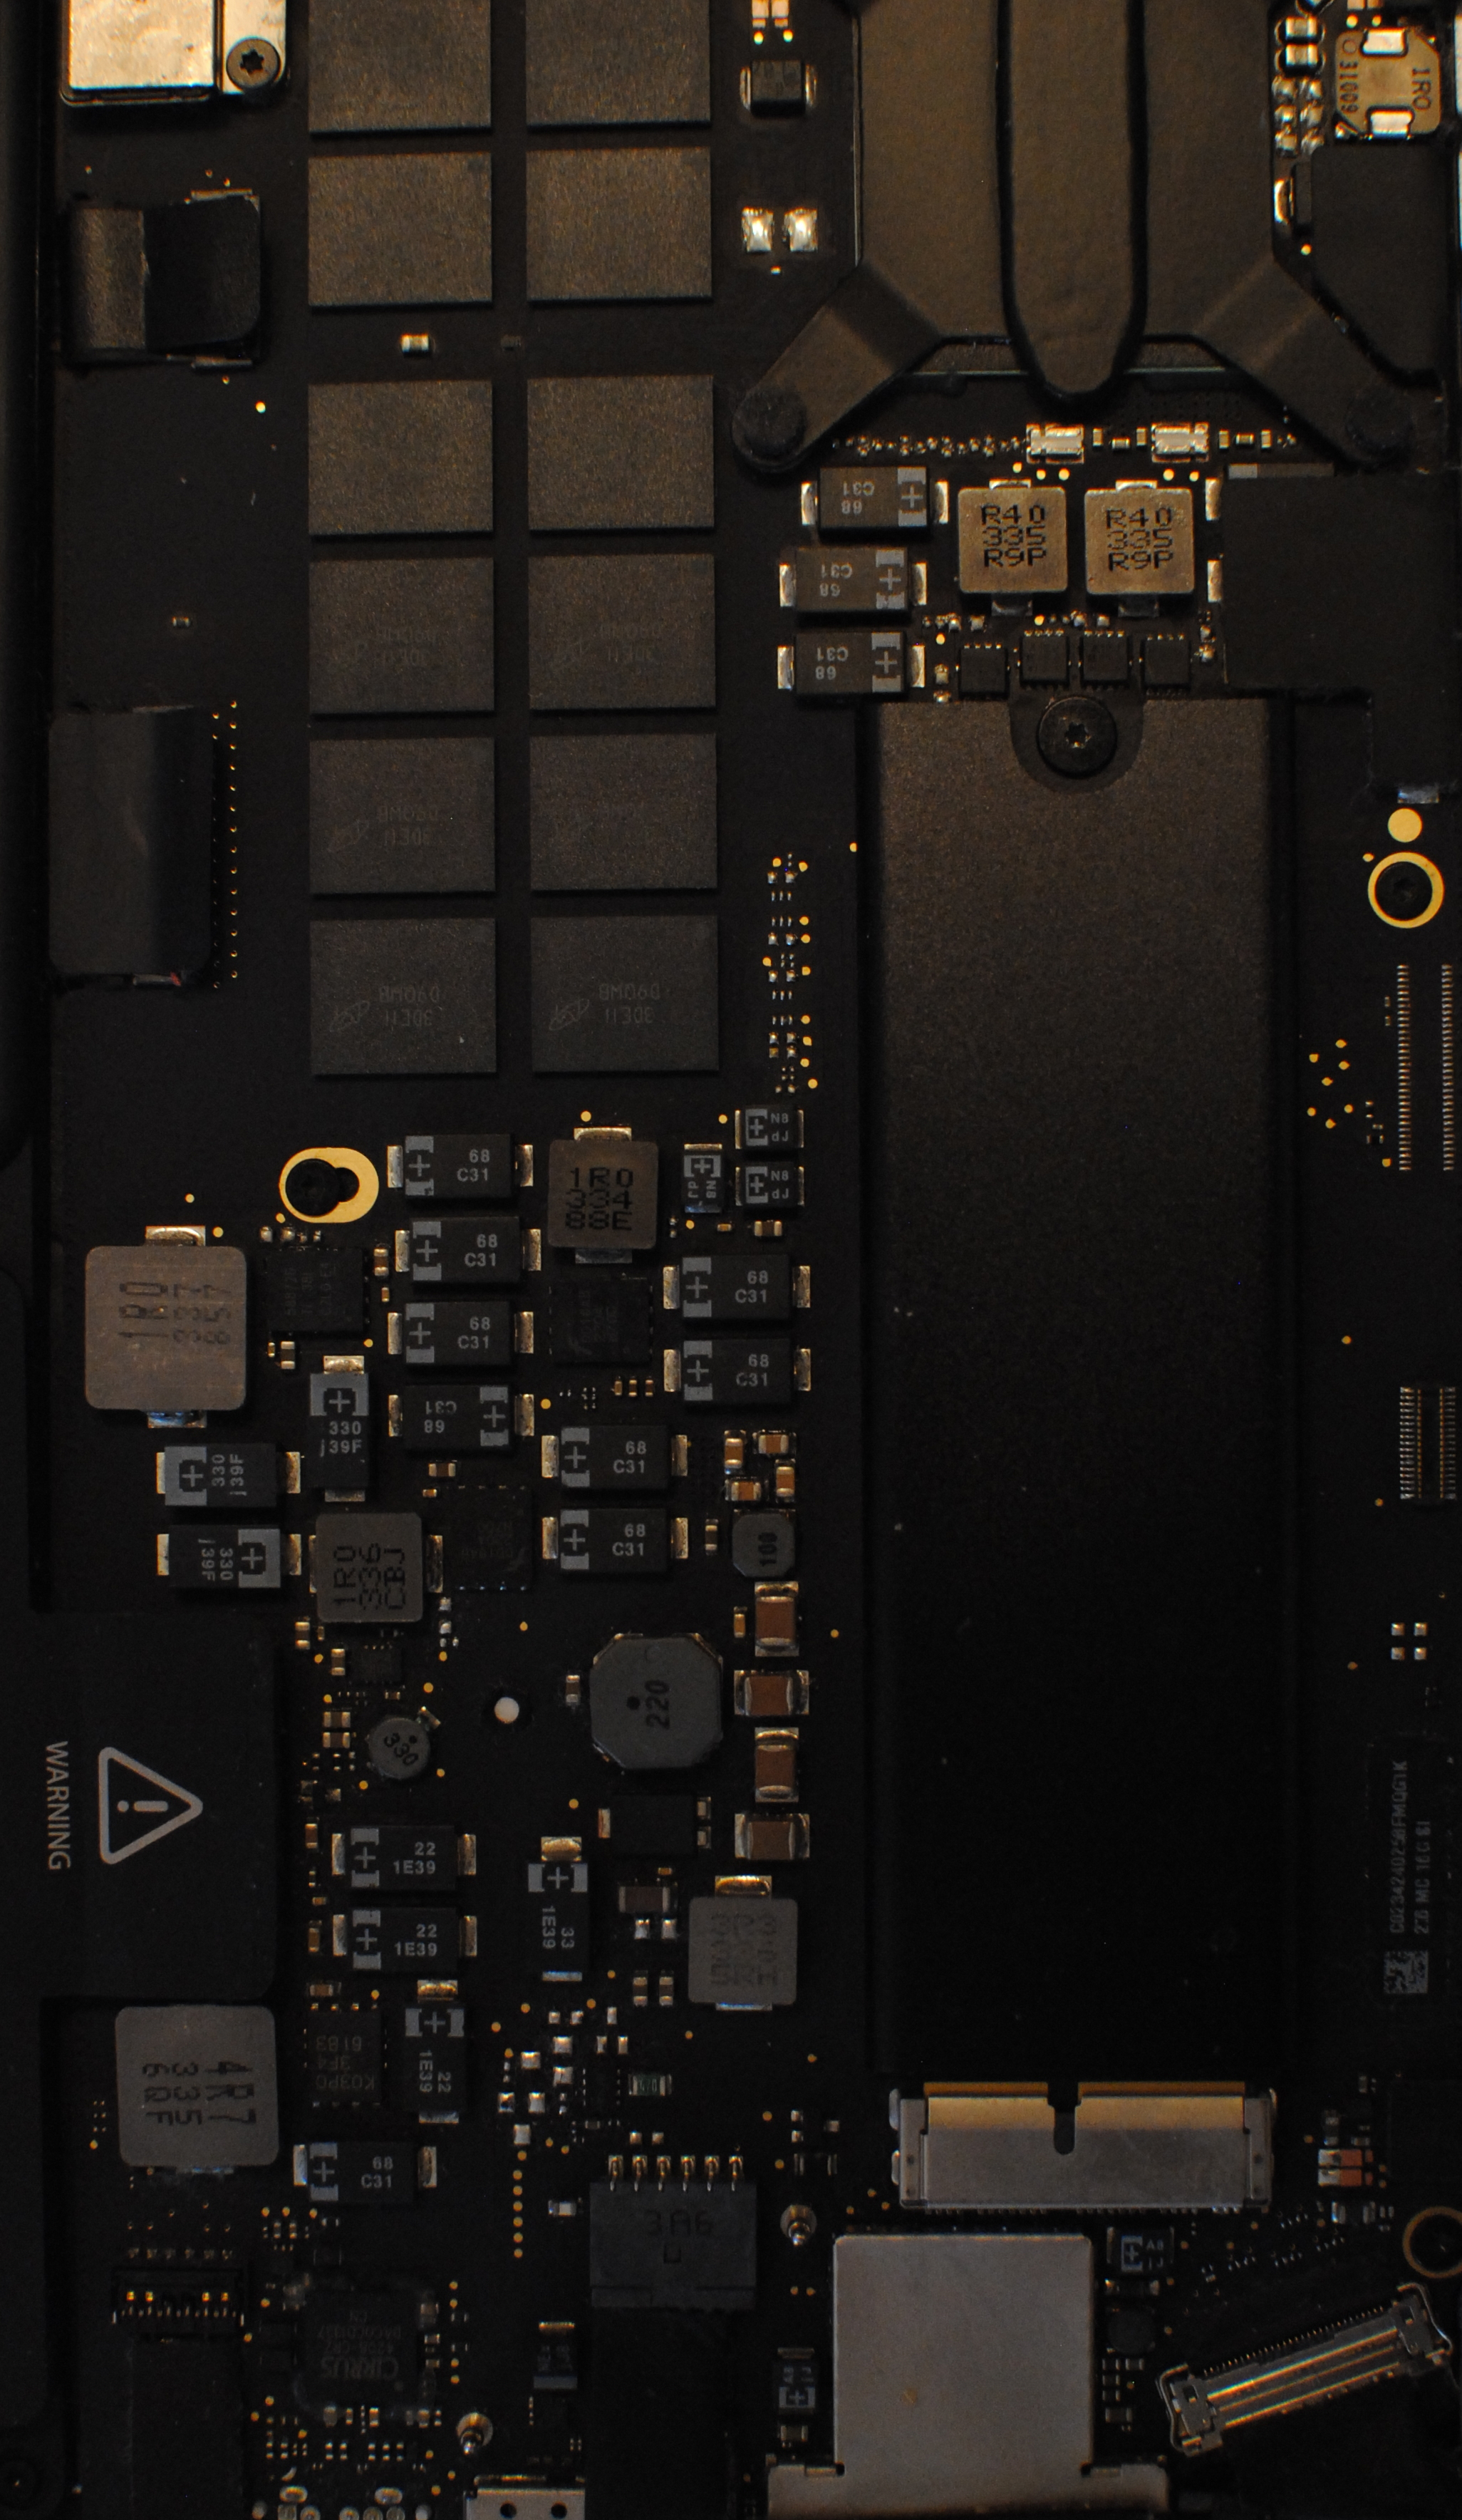
\includegraphics[scale=0.2]{figures/experiments/img.JPG}}
    
        \subfloat[Some cool related graphic]
        {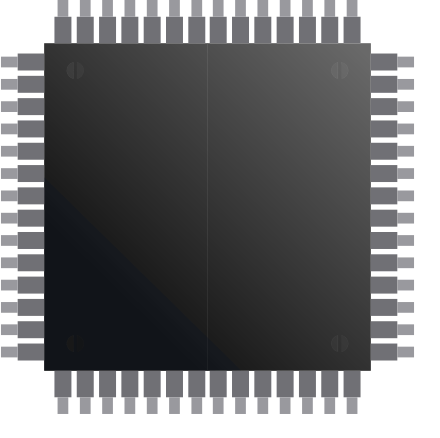
\includegraphics[scale=0.4]{figures/experiments/microcontroller.png}}
        \caption[Caption that appears in the figlist]{\textbf{Caption that appears under the fig} \lipsum[1-1]}
        \label{fig:pcaclasses}
    \end{centering}
\end{figure}

% \begin{table}[ht]
\centering
% spacing in table
\ra{1.3}
\begin{tabular}{@{}lr@{}}
  \toprule
  Type & Accuracy\\ \midrule
  A    & 82.47 $\pm$ 3.21 \\
  B    & 78.47 $\pm$ 2.43 \\
  C    & 84.30 $\pm$ 2.35 \\
  D    & 86.81 $\pm$ 3.01 \\
  \bottomrule
\end{tabular}

    \caption[Table caption]{\textbf{Table caption.} foo bar...\\}
    \label{tab:accuracy}
\end{table}

\section{VAE}

In the folling section I will present the results of my experiments with the Variational-Autoencoder to encode and decode actions from the environment.
Consistent over all experiments with the VAE sizes of the datasets are consistent:
\begin{itemize}
    \item train: 10.000 actions
    \item validation: 2000 actions
    \item test: 1000 action
\end{itemize}


\subsection{Pure Actions}

In every state of the sequential decision making process there are multiple actions available to go from the current state $s_t$ to the next state $s_{t+1}$ where the arm end position is at the goal position. To gain a dataset that contains such actions I sampled the robot arm angles in $s_t$ from a uniform distribution $\mathcal{U}_[0, 2\pi]$ and applied the CCD algorithm to get access to the action that leads from $s_t$ to $s_{t+1}$ with the robot arm end position near the goal state.\\

The results of the training process are shown in \figref{}

\subsection{Conditioning on States}

After watching the pure action encoding and decoding fail in the all important reconstruction loss. I got inspired by the paper \todo{cite LASER} and rerolled the experiments with an conditional Variational-Autoencoder where the conditional information is the information from $s_t$. 
The results of the training process are shown in \figref{}

We can observe that the test reconstruction loss is much lower that before and the kl loss

\begin{table}[]
    \centering
    \begin{tabular}{l|l|r|r}
         n & latent dim & r loss & kl loss\\
         2 & 2 & & \\
         2 & 1 & & \\
         5 & 5 & & \\
         5 & 4 & & \\
         5 & 3 & & \\
         5 & 2 & & \\
         5 & 1 & & \\
         10 & 2 & & \\
         10 & 2 & & \\
         10 & 2 & & \\
         10 & 2 & & \\
    \end{tabular}
    \caption{n is the number of joints, latent dimension is the size of the dimension the action is compressed to, r loss is the test reconstruction loss I used the MSE as the metric for the reconstruction loss, kl loss is the Kullback Leiber diveregence from the standard normal distribution on the test dataset}
    \label{tab:CVAE results}
\end{table}
\todo{Concering the table: make a lot of experiments so I can get an std ?, or should I just say that the training turns out to be not as stable as it should be in comparison to an VAE on MNIST and that we sampled runs until we got a good result?}

\subsection{Fitting Random Noise}

In this section I will present the results on how we tried to encode and decode actions sampled from a parameterized distributuion.
The idea is that in every state the agent can choose an action from $[-1, 1]^n$. Therefor I sampled a dataset independent and identically distributed from $\mathcal{U}^n_{[-1, 1]}$. this could be describe of trying to fit random noise.
The results for 800 epochs are shown in \figref{}.


\section{SAC}

\subsection{Hyperparameters}

\begin{table}[]
    \centering
    \begin{tabular}{l|l}
         name & values \\
         \hline
         task & ReachGoalTask, ImitationTask \\
         lr pi & 0.0005 \\
         lr q & 0.001 \\
         init alpha & 0.01 \\
         gamma & 0.98, 0  \\
         batch size & 32 \\
         buffer limit & 50000 \\
         start buffer size & 1000 \\
         train iteration & 20 \\
         tau & 0.01 \\ 
         target entropy & -40.0 \\
         lr alpha & 0.001 \\
         n epochs & 5000 \\
         action covariance mode & independent \\
         action covariance decay &  0.5 \\
         action magnitude & 0.1 \\
        \end{tabular}
    \caption{Hyperparameters for the Soft-Actor-Critic algorithm}
    \label{tab:Hyperparameters}
\end{table}
\todo{description?}

\subsection{Baseline}

In this section I want to present the results of the baseline experiments. To mimic a sequential decision making process and constrain the actions I manually tuned the parameter ``action magnitude'' between 1, 0.5, 0.2, and 0.1. The results are shown in figures: \figref{}

Stichworte die rein sollen
- Mit erhörter Anzahl an joint wid die Performance ober alle experimente immer schlechter
- Affällig hohe Varianz bei kleiner werdeneder Anzahl joint
- Absacken der Performance von 2 joints mit weiter Erniedrigung der action magnitude
- 5 joints scheinen eine ähnliche Performance über die action magnitude abzu geben
- Scheinbar habe ich bei 0.2 einen Wert gefunden der auch für höhere Anzahlen von joints gut zu funktionieren scheint. -> Fahre daher weiter mit diesem Parameter fort.

\begin{figure}
    \begin{center}
        \subfloat[Mean reward per step over the last 20 episodes.]{
            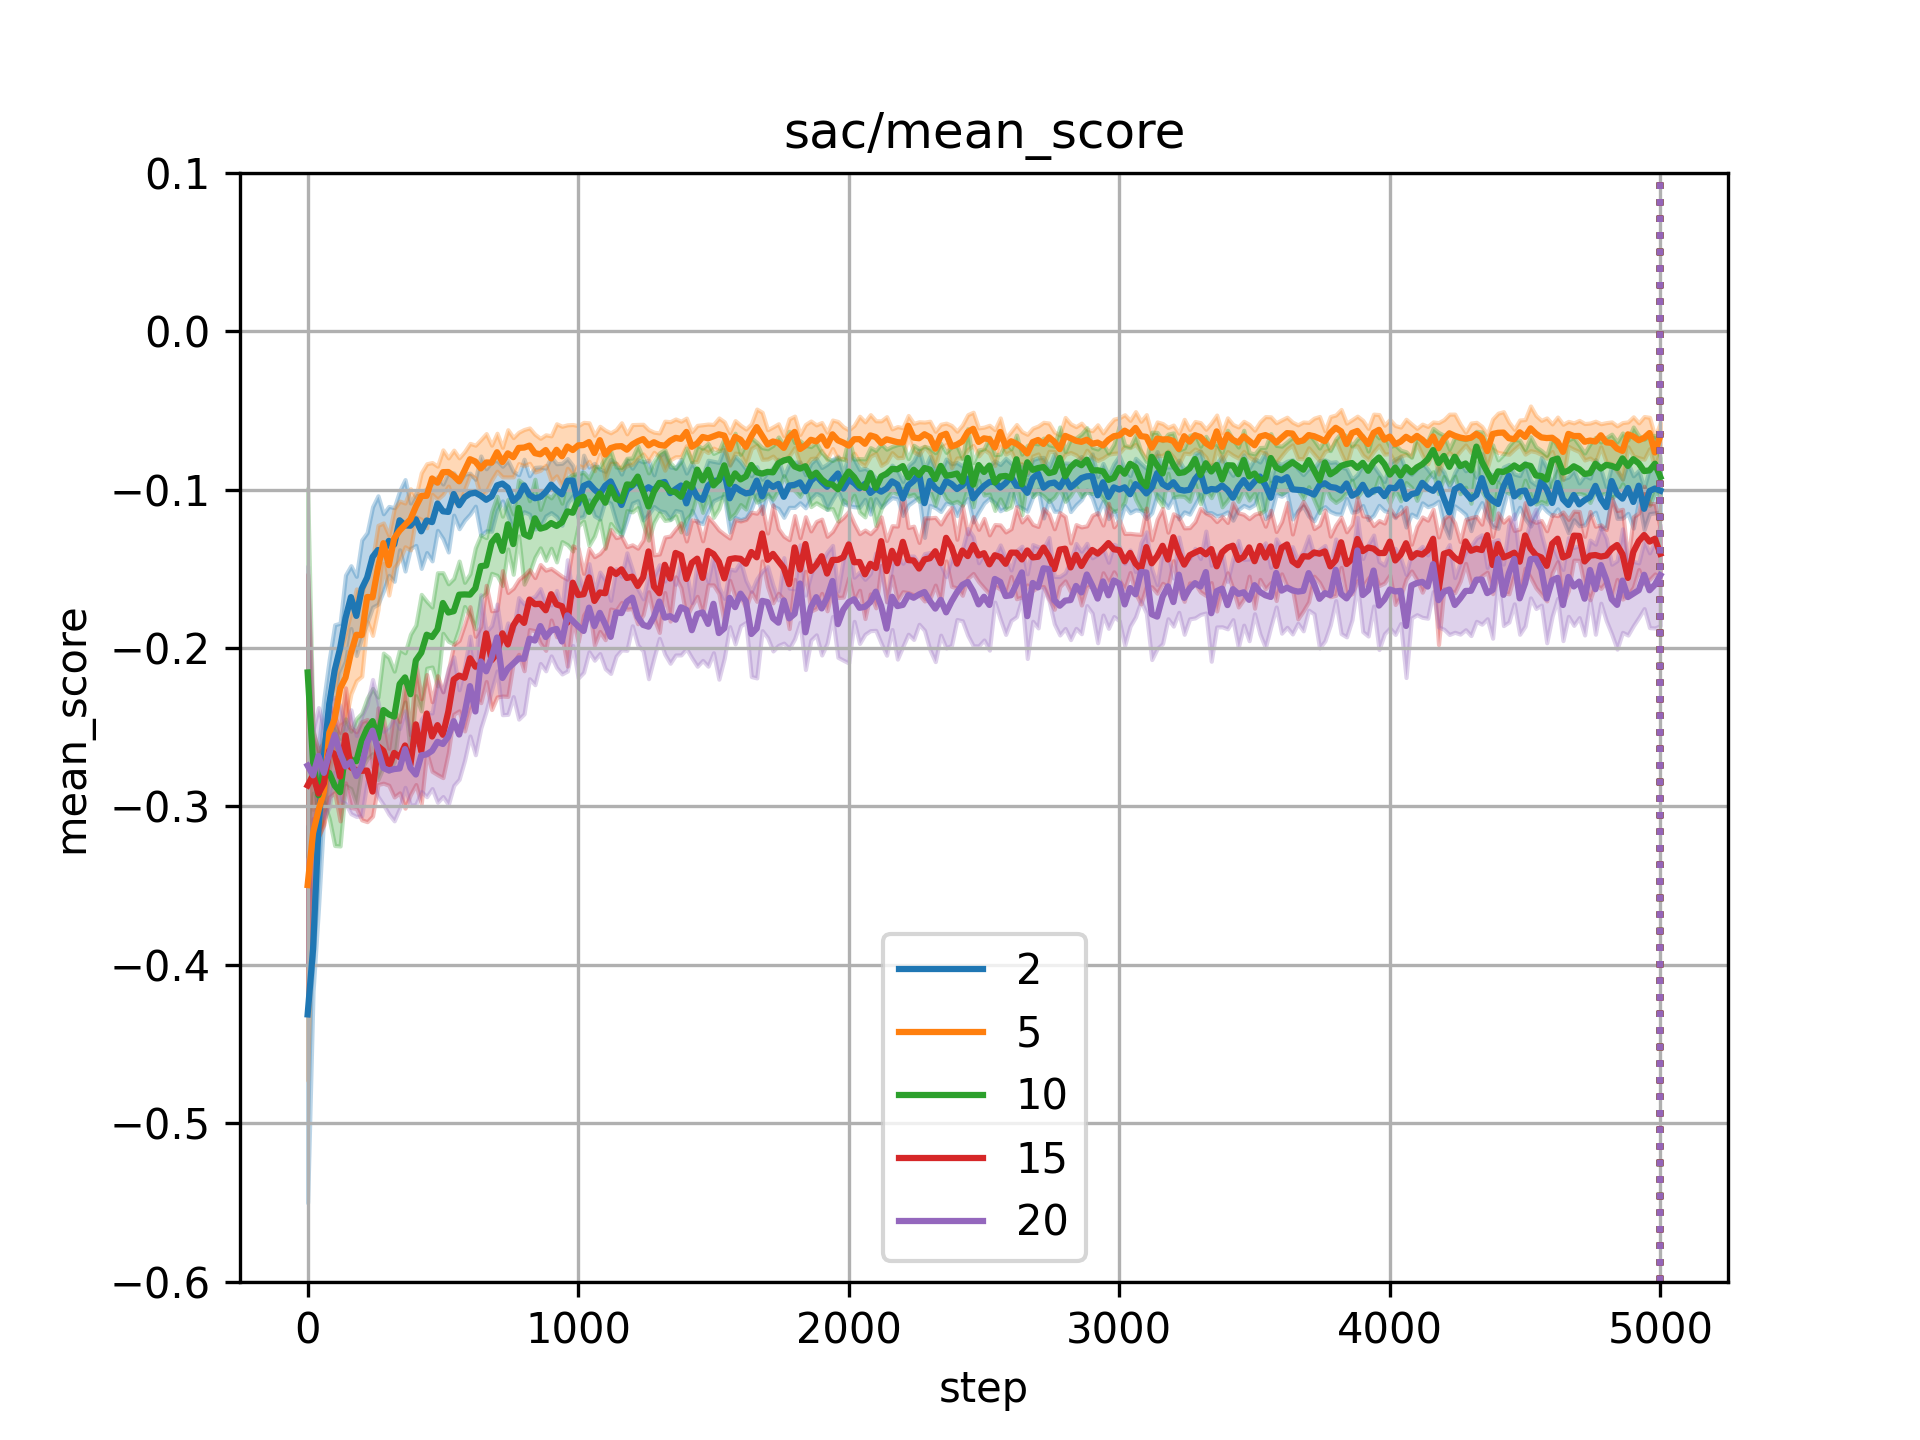
\includegraphics[width=0.46 \linewidth]{figures/experiments/sac_baseline_mean_score.png}
            \label{fig:SAC_baseline/reward}
            }
        \hfill
        \subfloat[Mean episode length over the last 20 episodes]{
        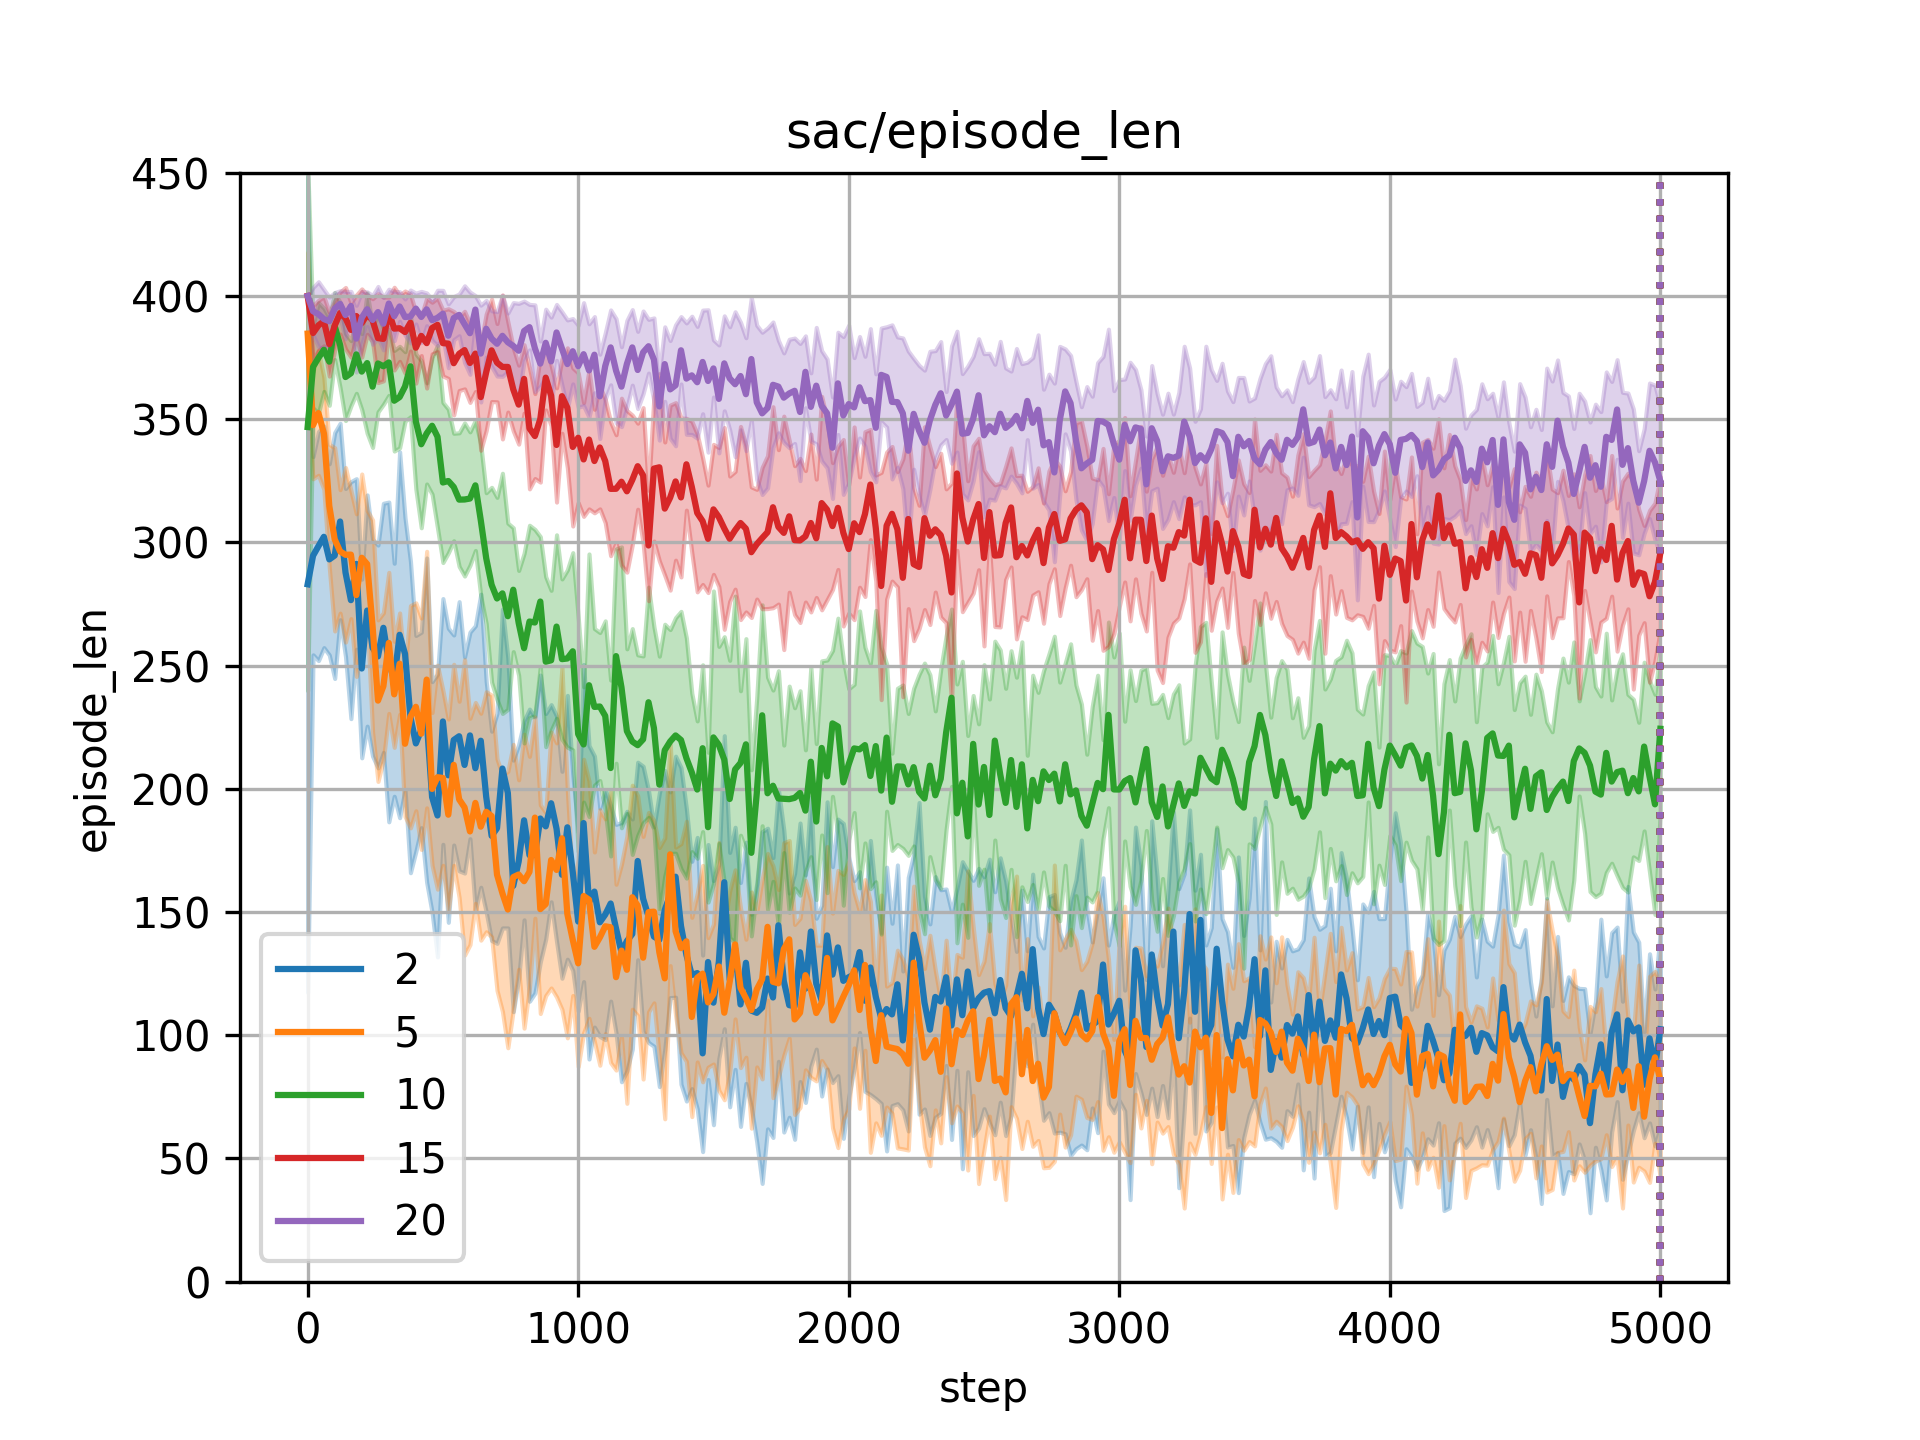
\includegraphics[width=0.46 \linewidth]{figures/experiments/sac_baseline_episode_len.png}
            \label{fig:SAC_baseline/episode_len}
            }
    \end{center}
    \caption[SAC baseline experiment results]{SAC baseline experiment results with an increasing number of joints. We can clearly see that the algorithm does not scale well with an increasing number of joints and therefor drops in performance. Each experiment was conducted 10 times and the shaded areas resemble the standard deviation around the mean.}
    \label{fig:SAC_baseline}
\end{figure}




    \chapter{Discussion}\label{chap:discussion}

In this section, we are going to discuss the before-presented results of the experiments. We focus hereby only on the results from the Reinforcement Learning section in \chapref{chap:experiments}.

\section{Baseline SAC}


Let's delve into the foundational results of the baseline SAC experiments. We immediately noticed a pronounced correlation between the performance of the SAC algorithm and the number of joints it was trained on. This connection is quite logical, as the effectiveness and computational demands of other inverse kinematics solvers, such as CCD, are intricately linked to the number of joints in the robotic system. This connection beautifully aligns with the runtime complexity analysis portrayed in \figref{fig:expert_dataset/runtime_complexity}.


\begin{figure}
    \begin{center}
        \subfloat[$N = 2$]{
            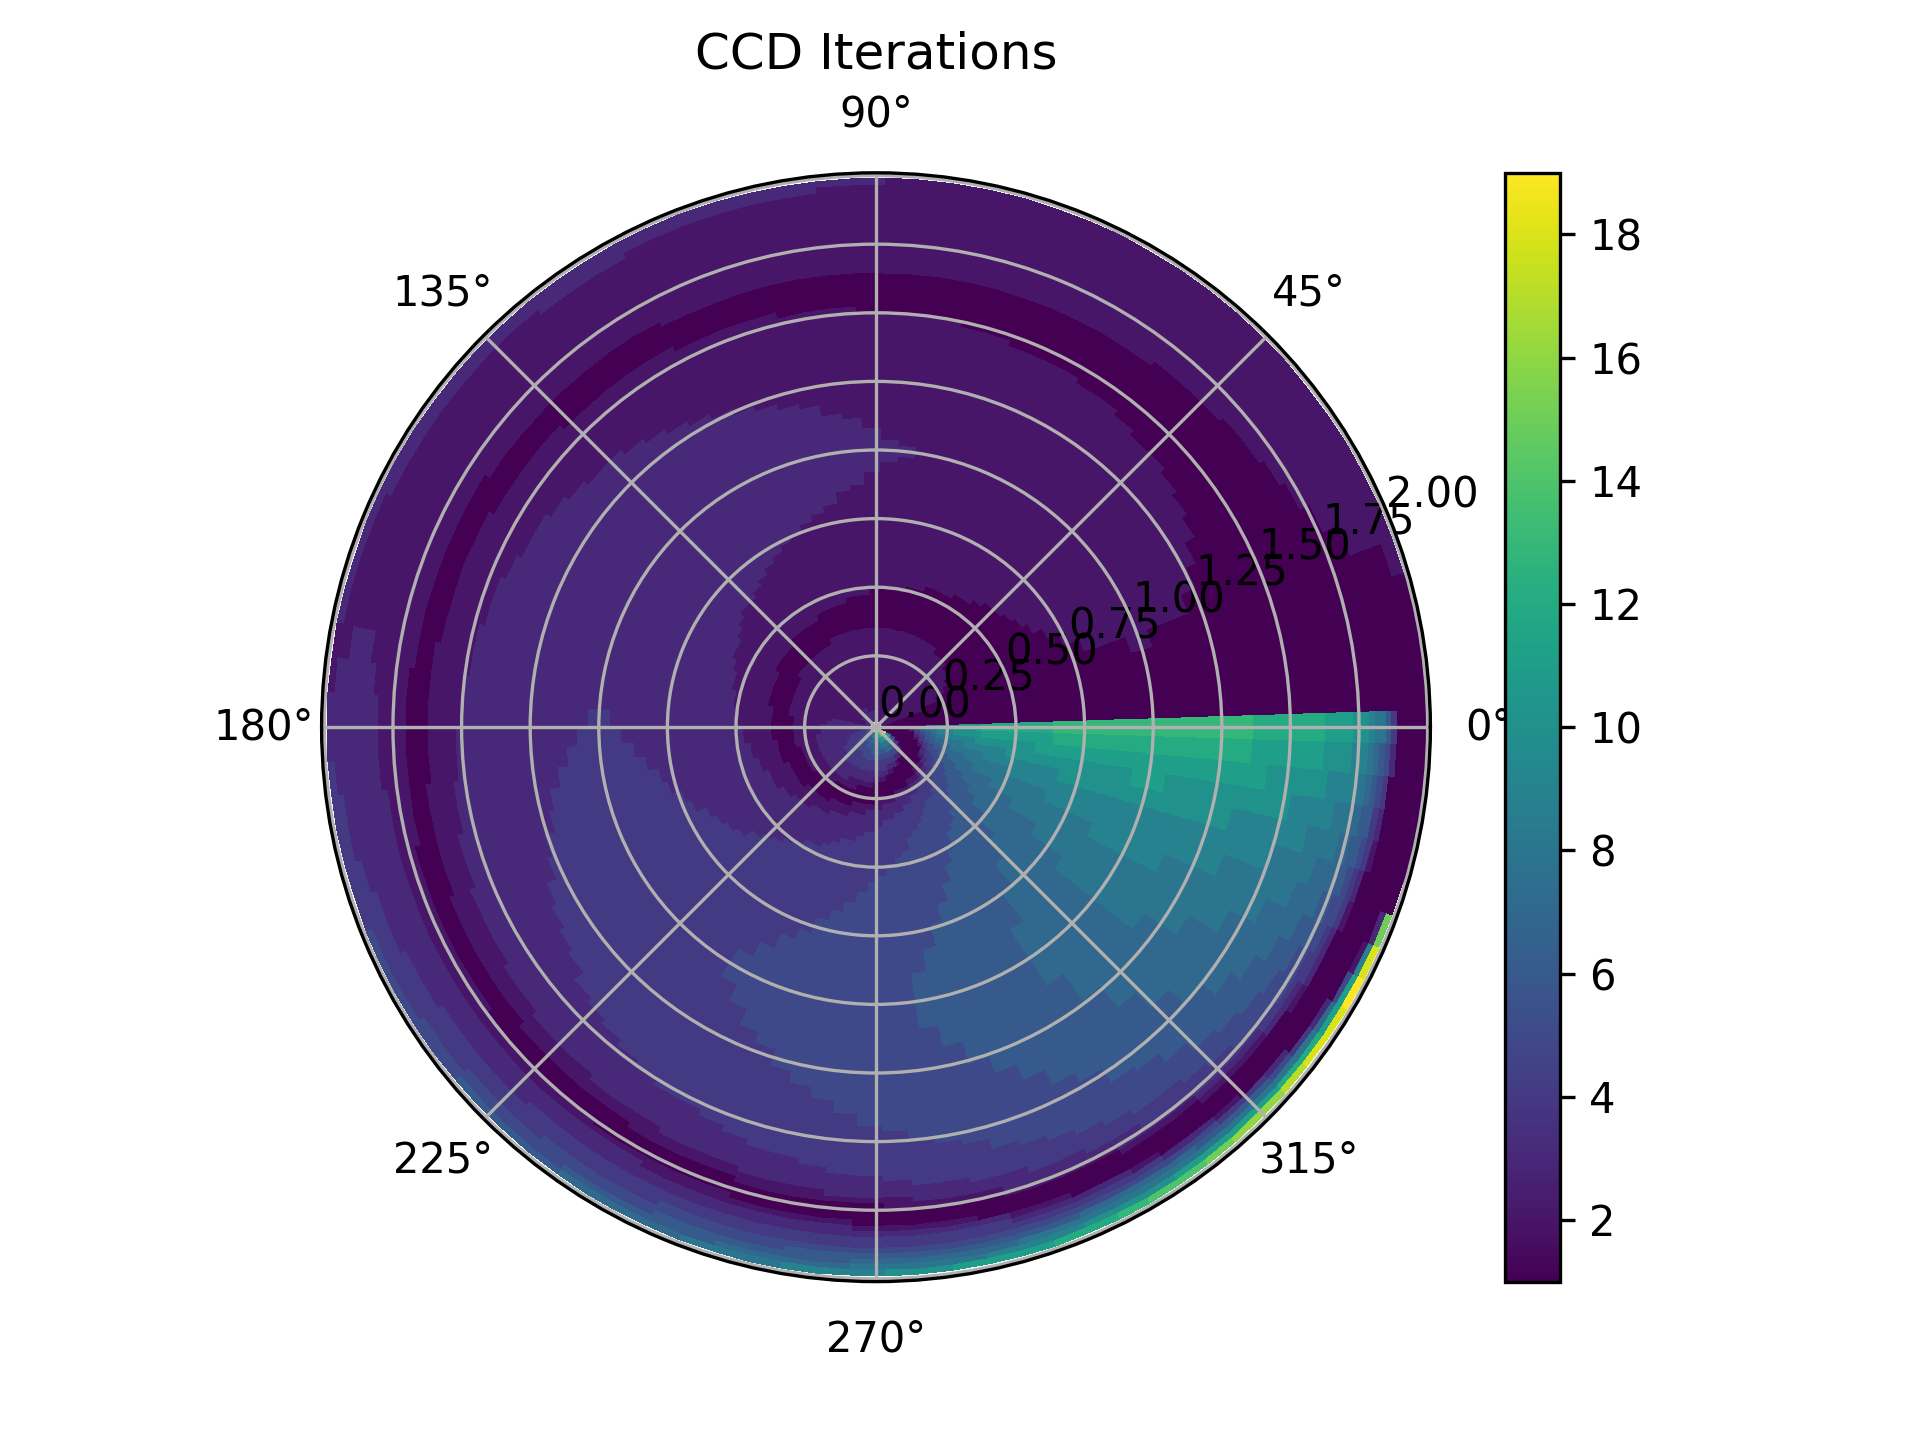
\includegraphics[width=0.31 \linewidth]{figures/background/CCD_2_iteration_heatmap.png}
            \label{fig:CCD_iteration/2}
            }
        \hfill
        \subfloat[$N = 5$]{
            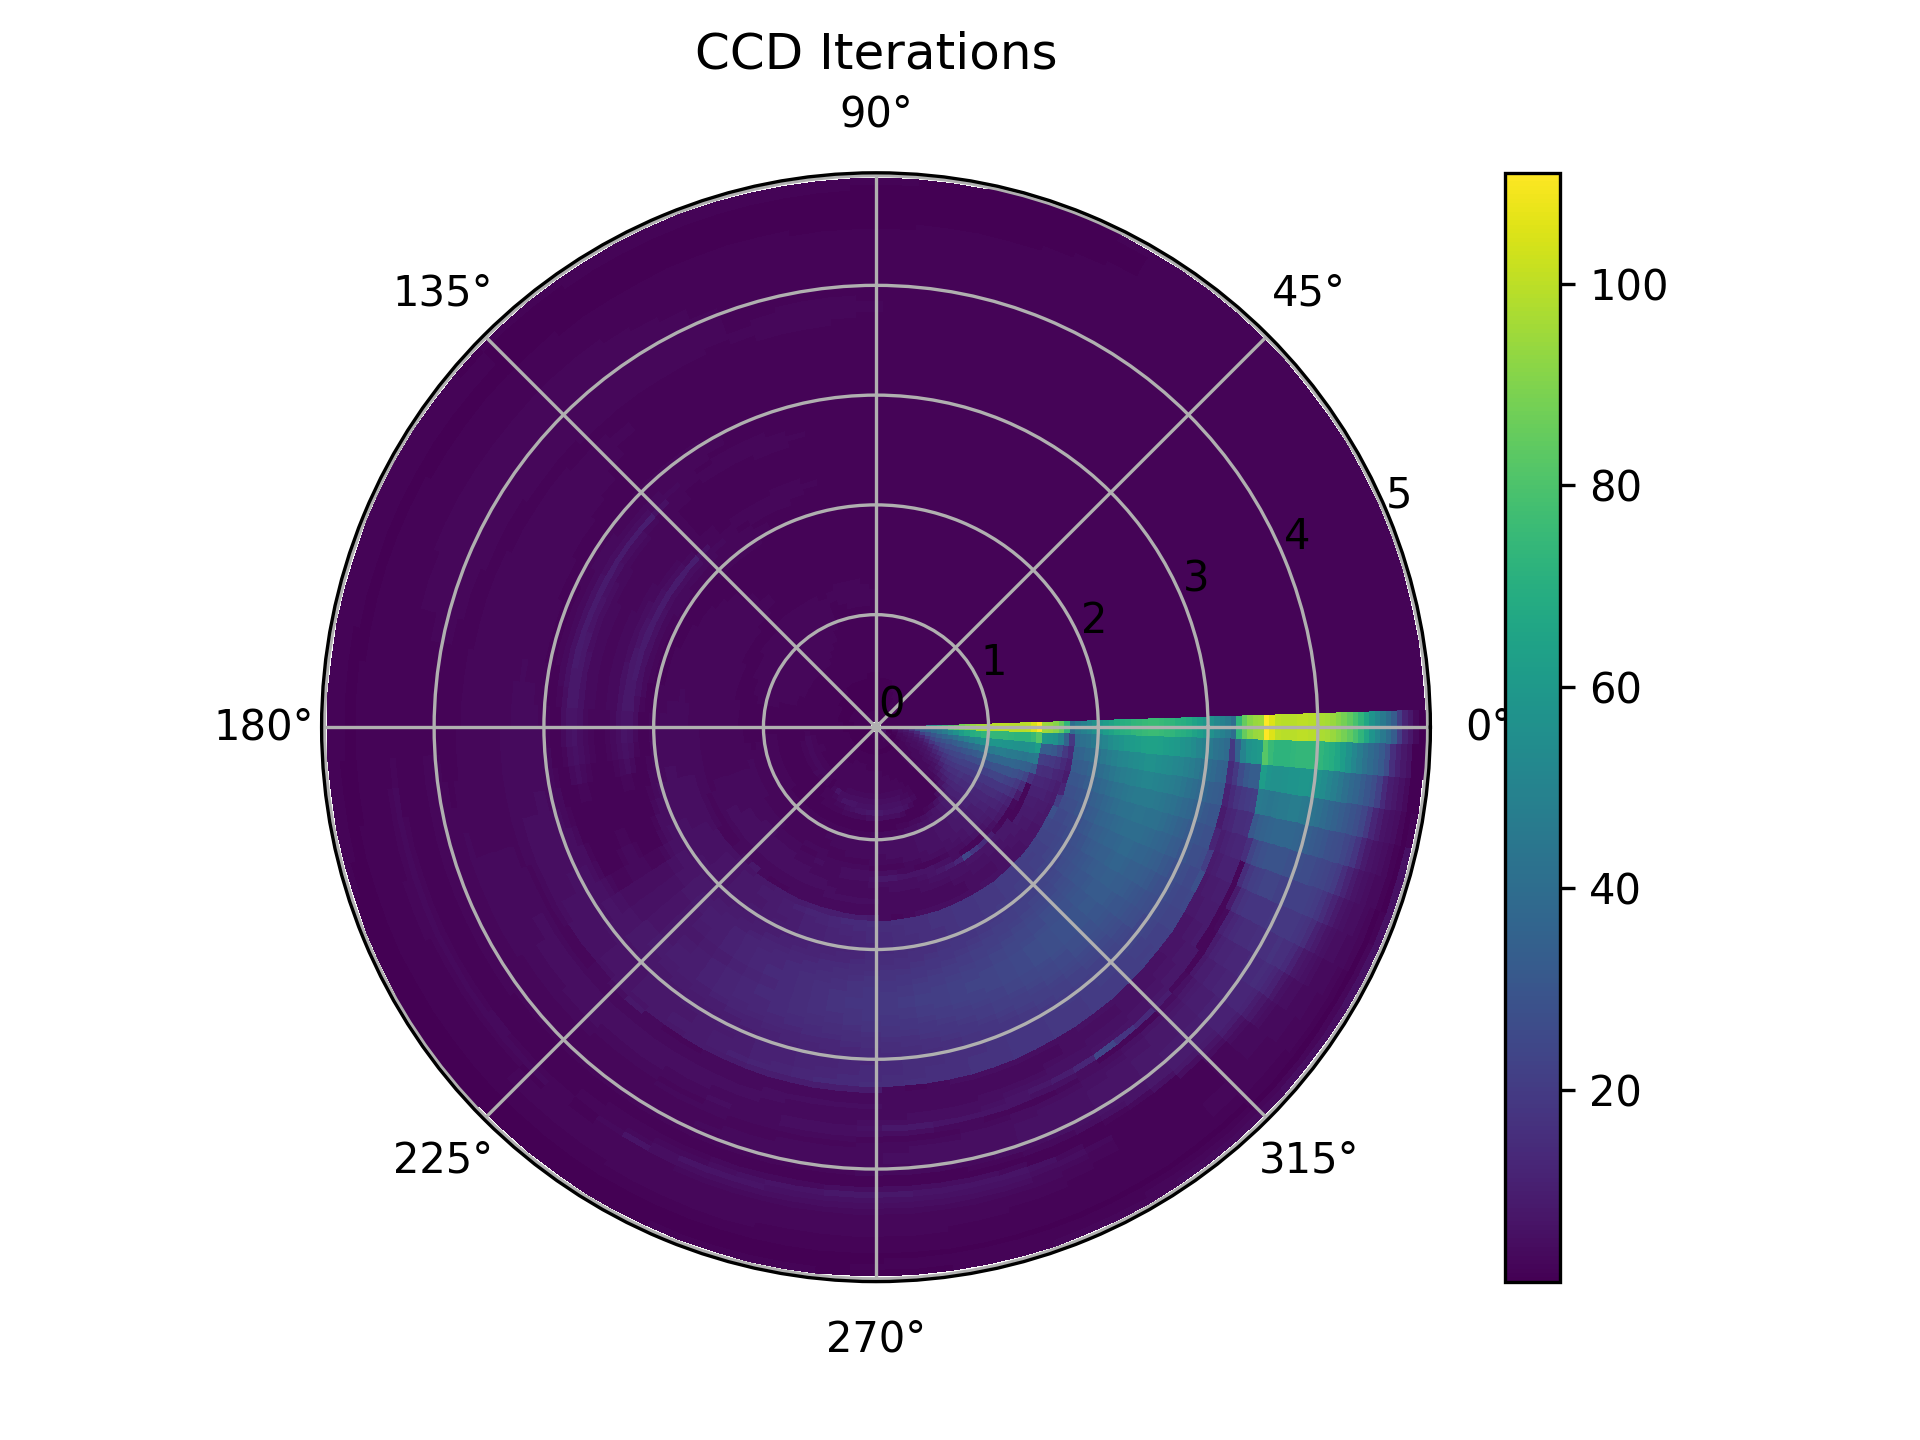
\includegraphics[width=0.31 \linewidth]{figures/background/CCD_5_iteration_heatmap.png}
            \label{fig:CCD_iteration/5}
            }
        \hfill
        \subfloat[$N = 10$]{
            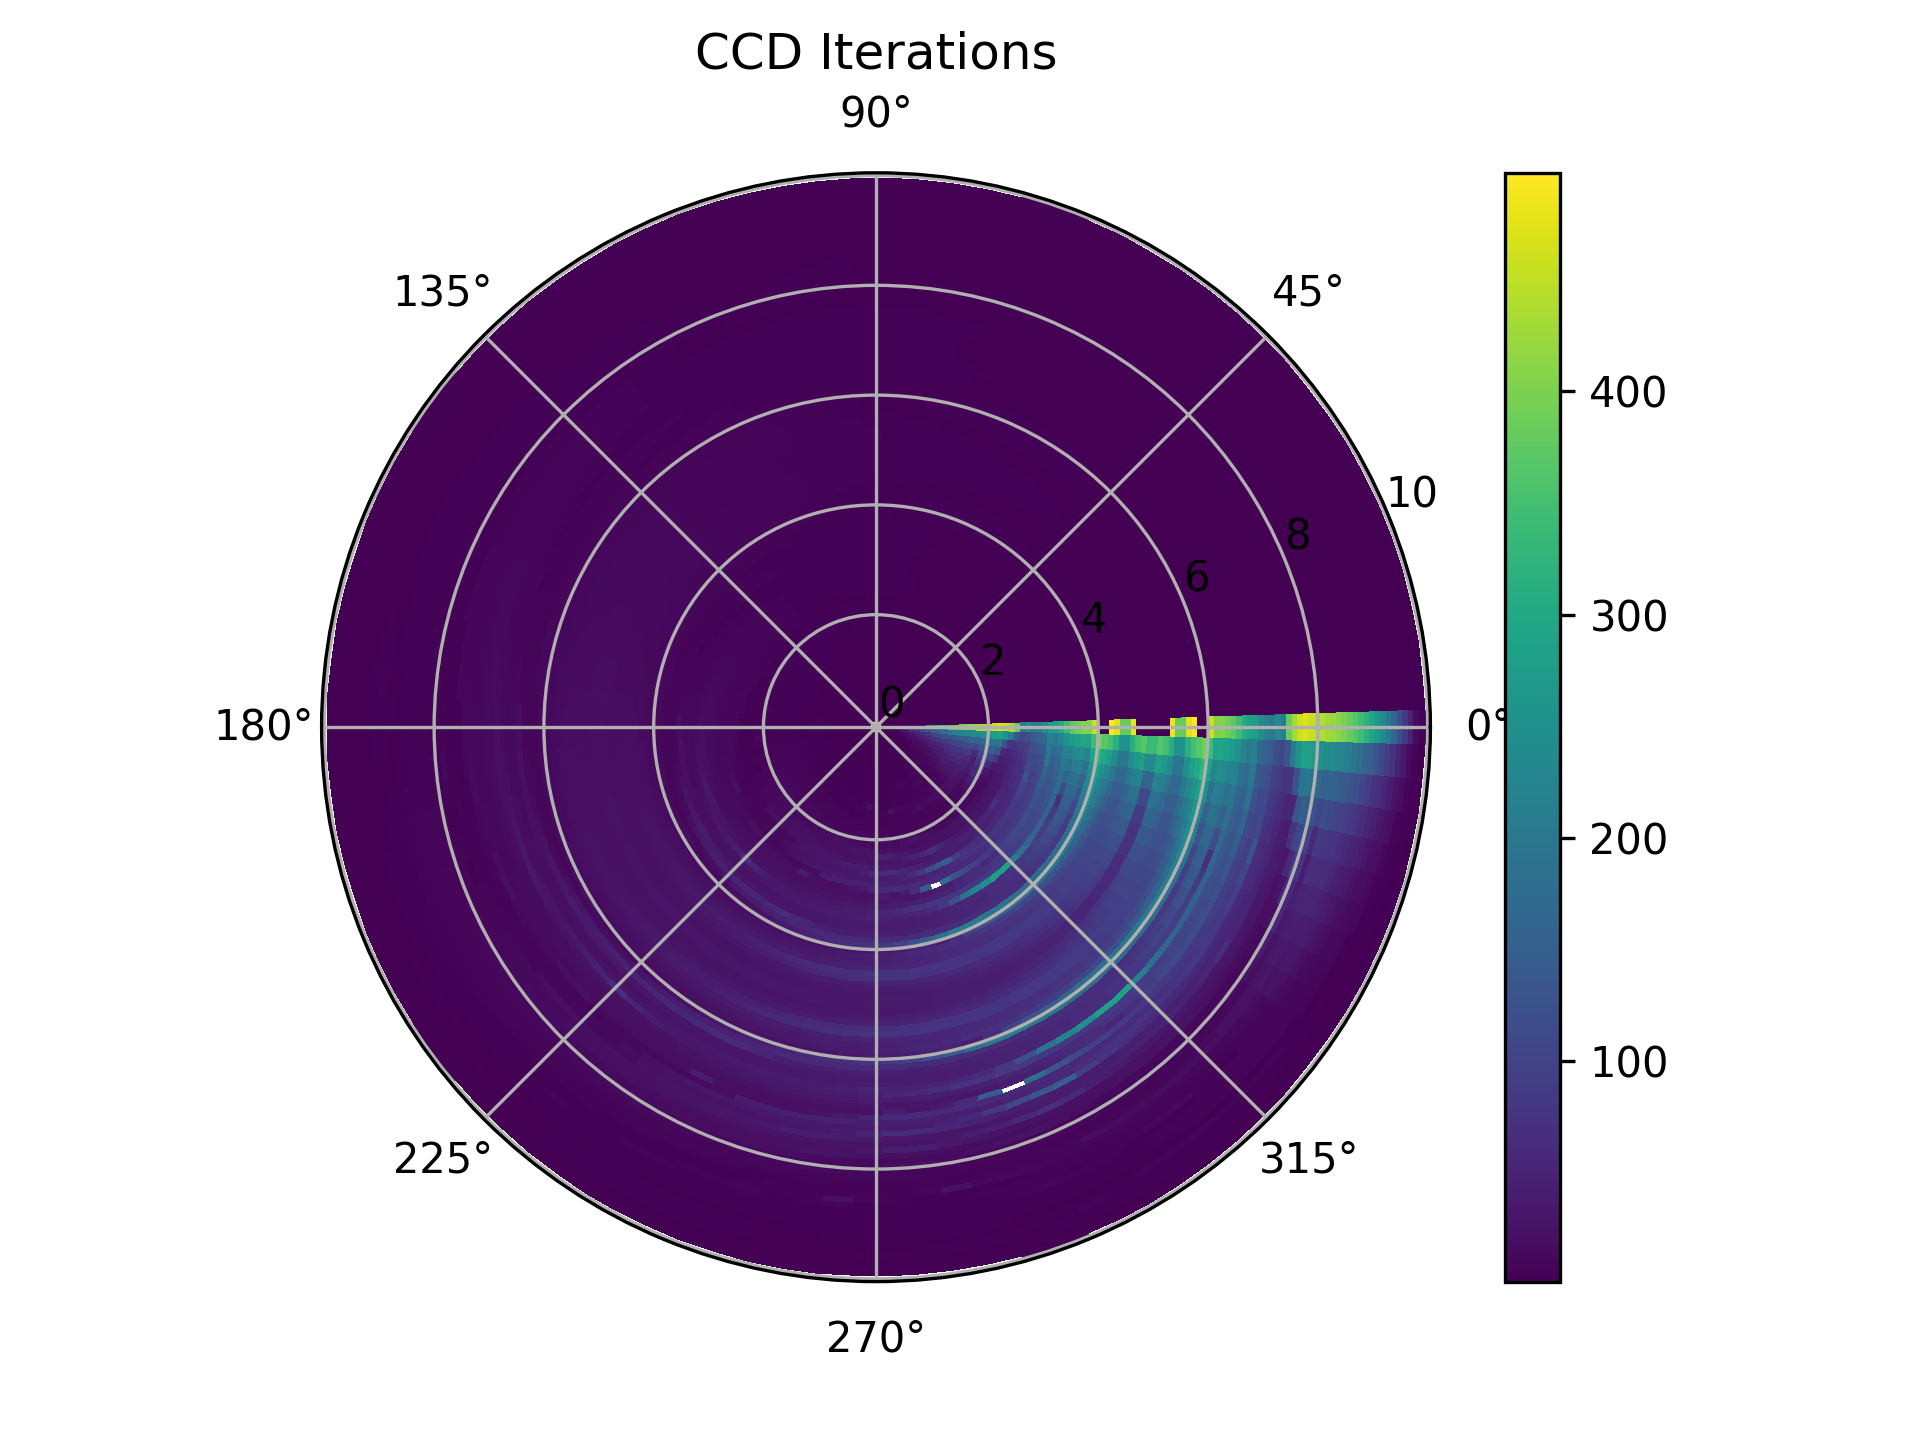
\includegraphics[width=0.31 \linewidth]{figures/background/CCD_10_iteration_heatmap.png}
            \label{fig:CCD_iteration/10}
            }
    \end{center}
    \caption[CCD iteration heatmap]{Heatmap of how many iterations CCD has needed to solve inverse kinematics starting from $[N, 0]$ targeting the middle of each polygon. The maximum budget is 20 times $N$ with a target precision of $0.1$.}
    \label{fig:CCD_iteration}
\end{figure}
\begin{figure}
    \begin{center}
        \subfloat[baseline. number of samples = 32062]{
            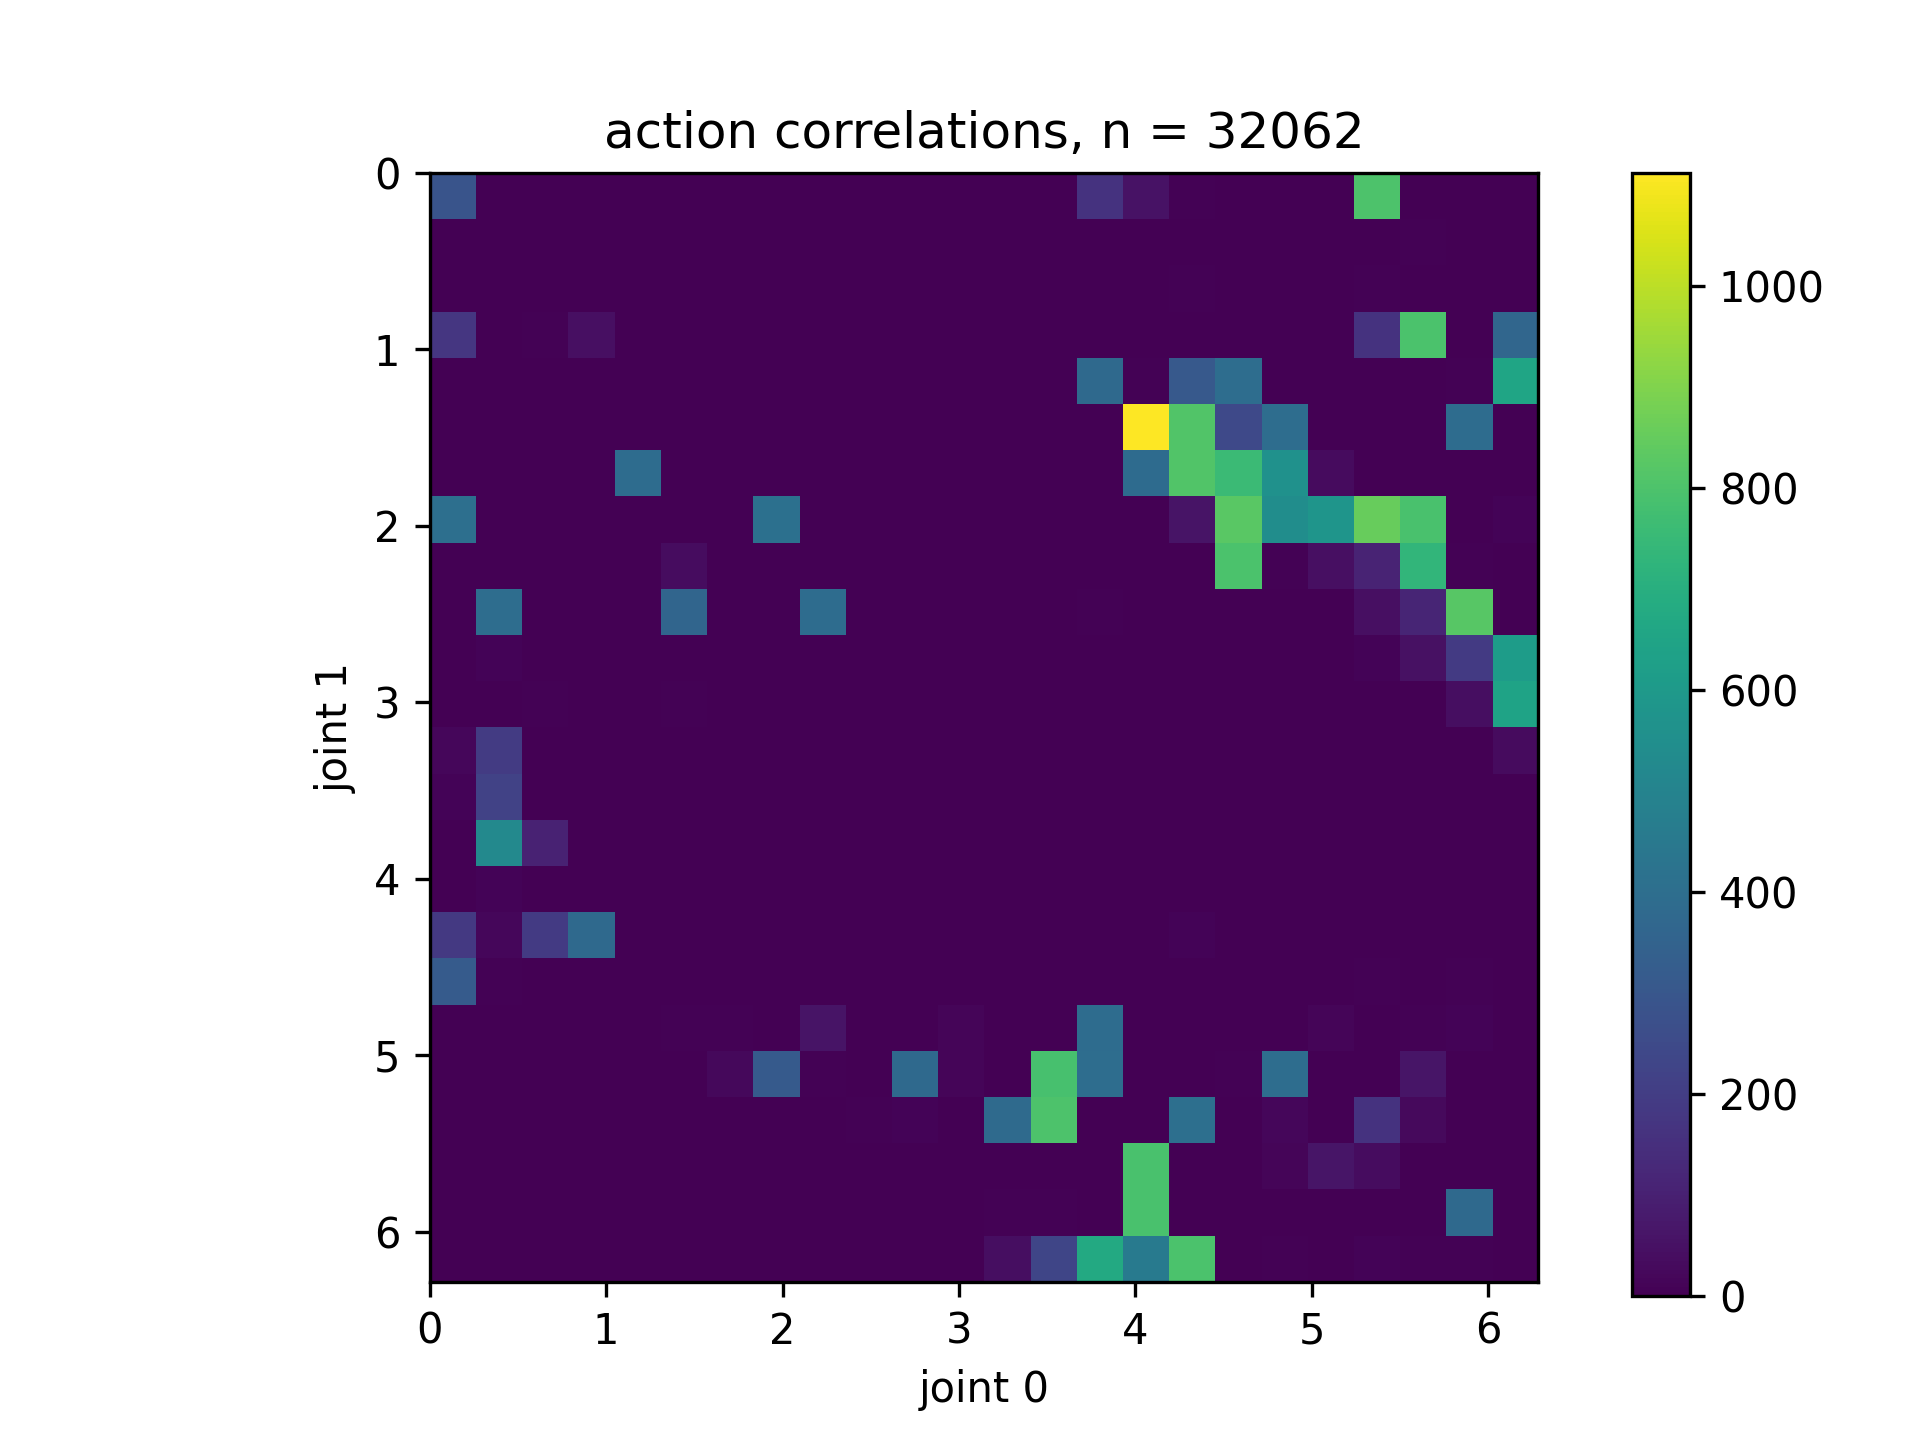
\includegraphics[width=0.23 \linewidth]{figures/experiments/action_correlations_baseline_2_1691621262_5000.png}
            \label{fig:SAC_action_correlation/baseline}
            }
        \hfill
        \subfloat[laten dimension is 2. number of samples = 39992]{
            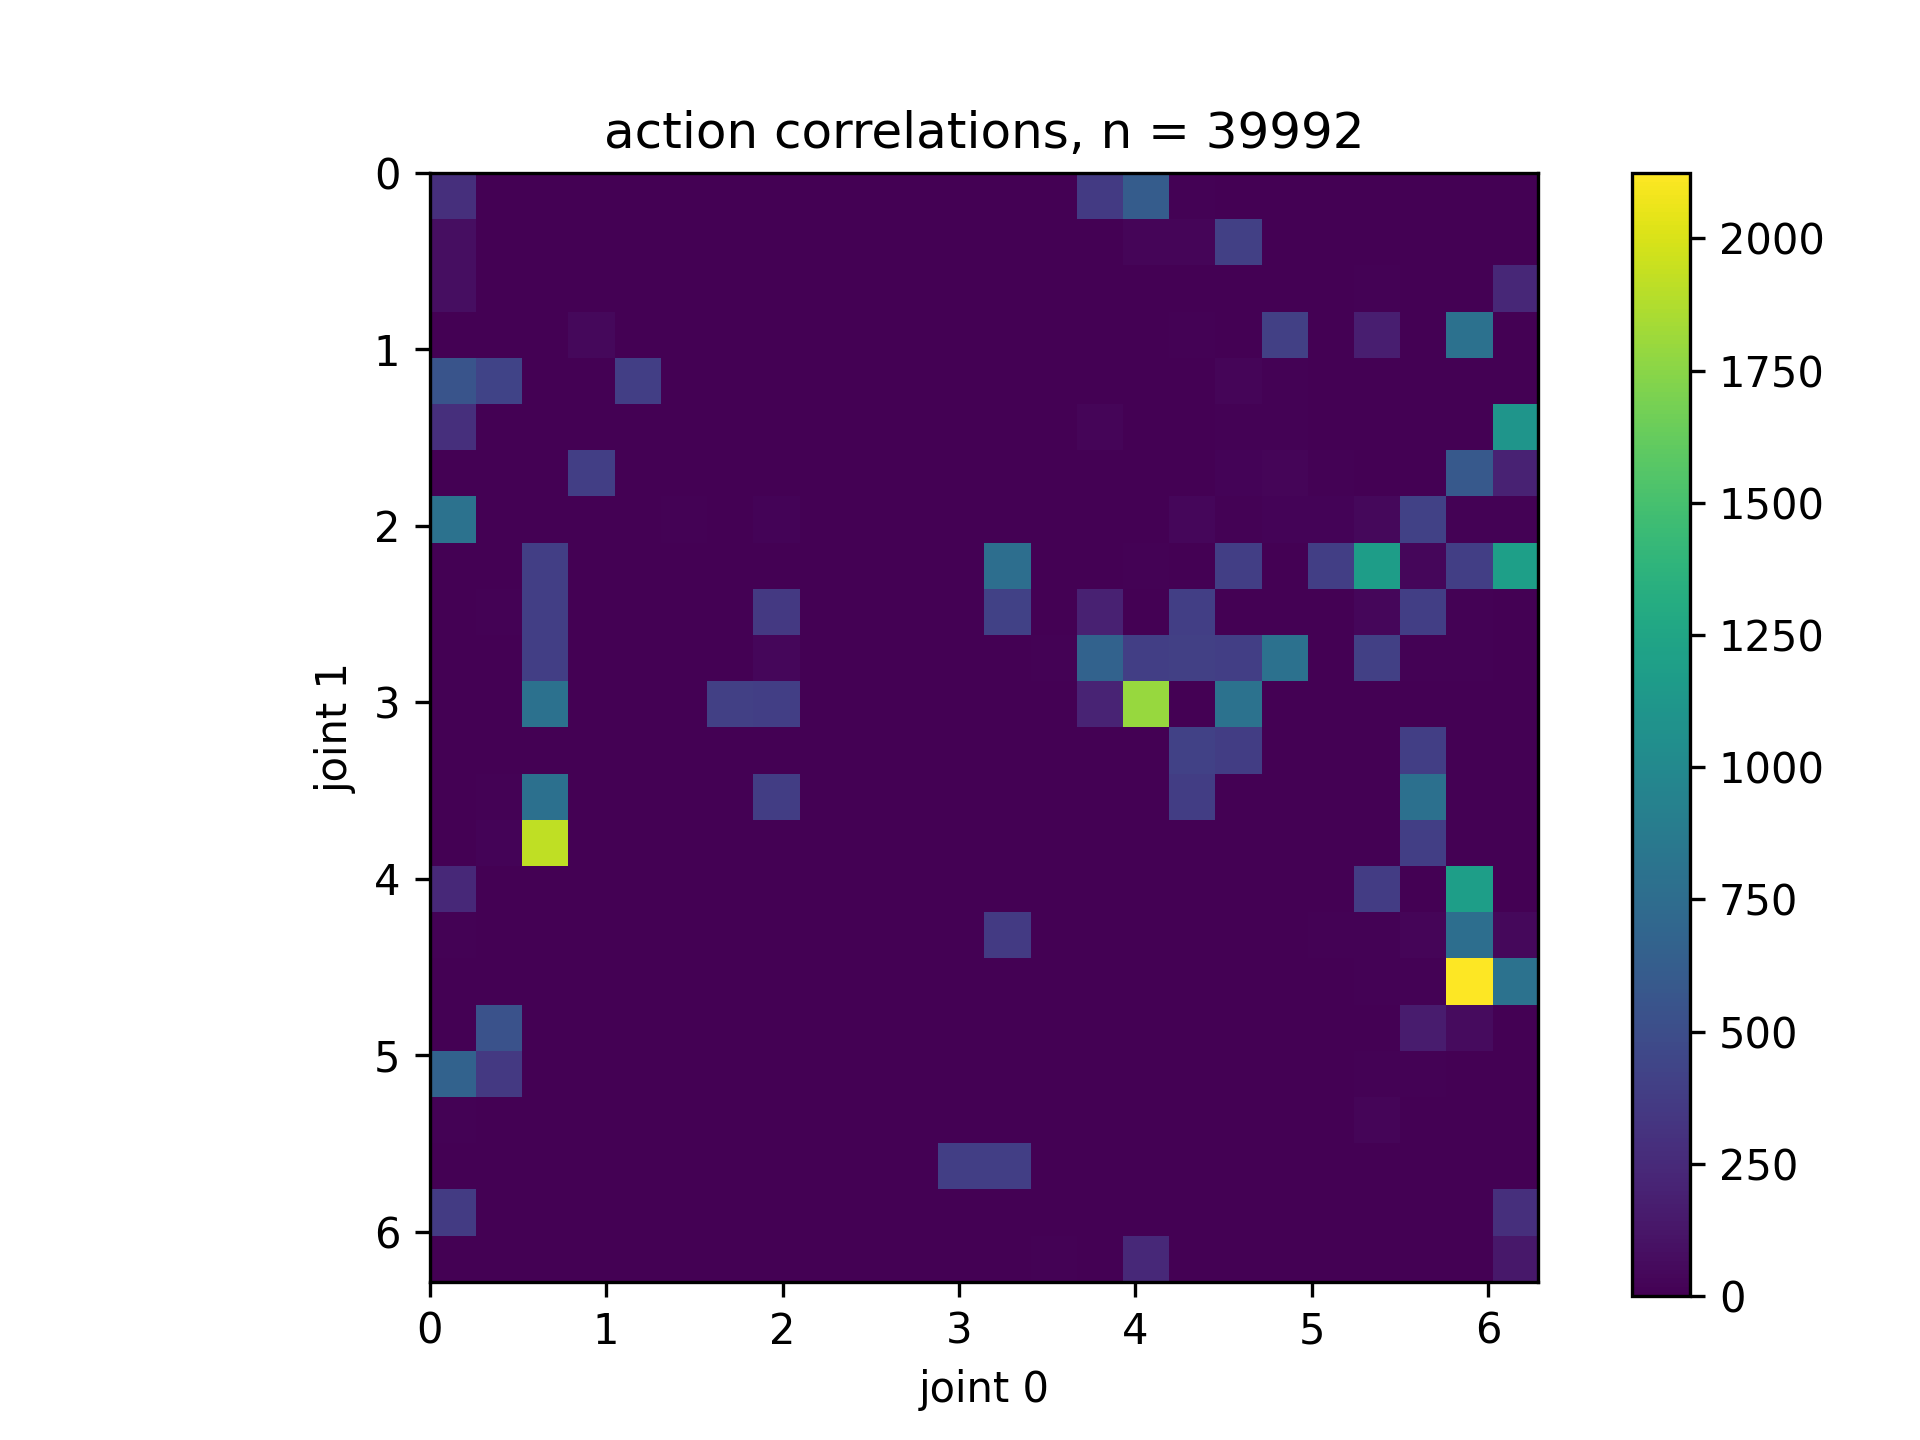
\includegraphics[width=0.23 \linewidth]{figures/experiments/action_correlations_latent_actor_2_2_1693146377_5000.png}
            \label{fig:SAC_action_correlation/latent_2}
            }
        \hfill
        \subfloat[laten dimension is 4. number of samples = 30810]{
            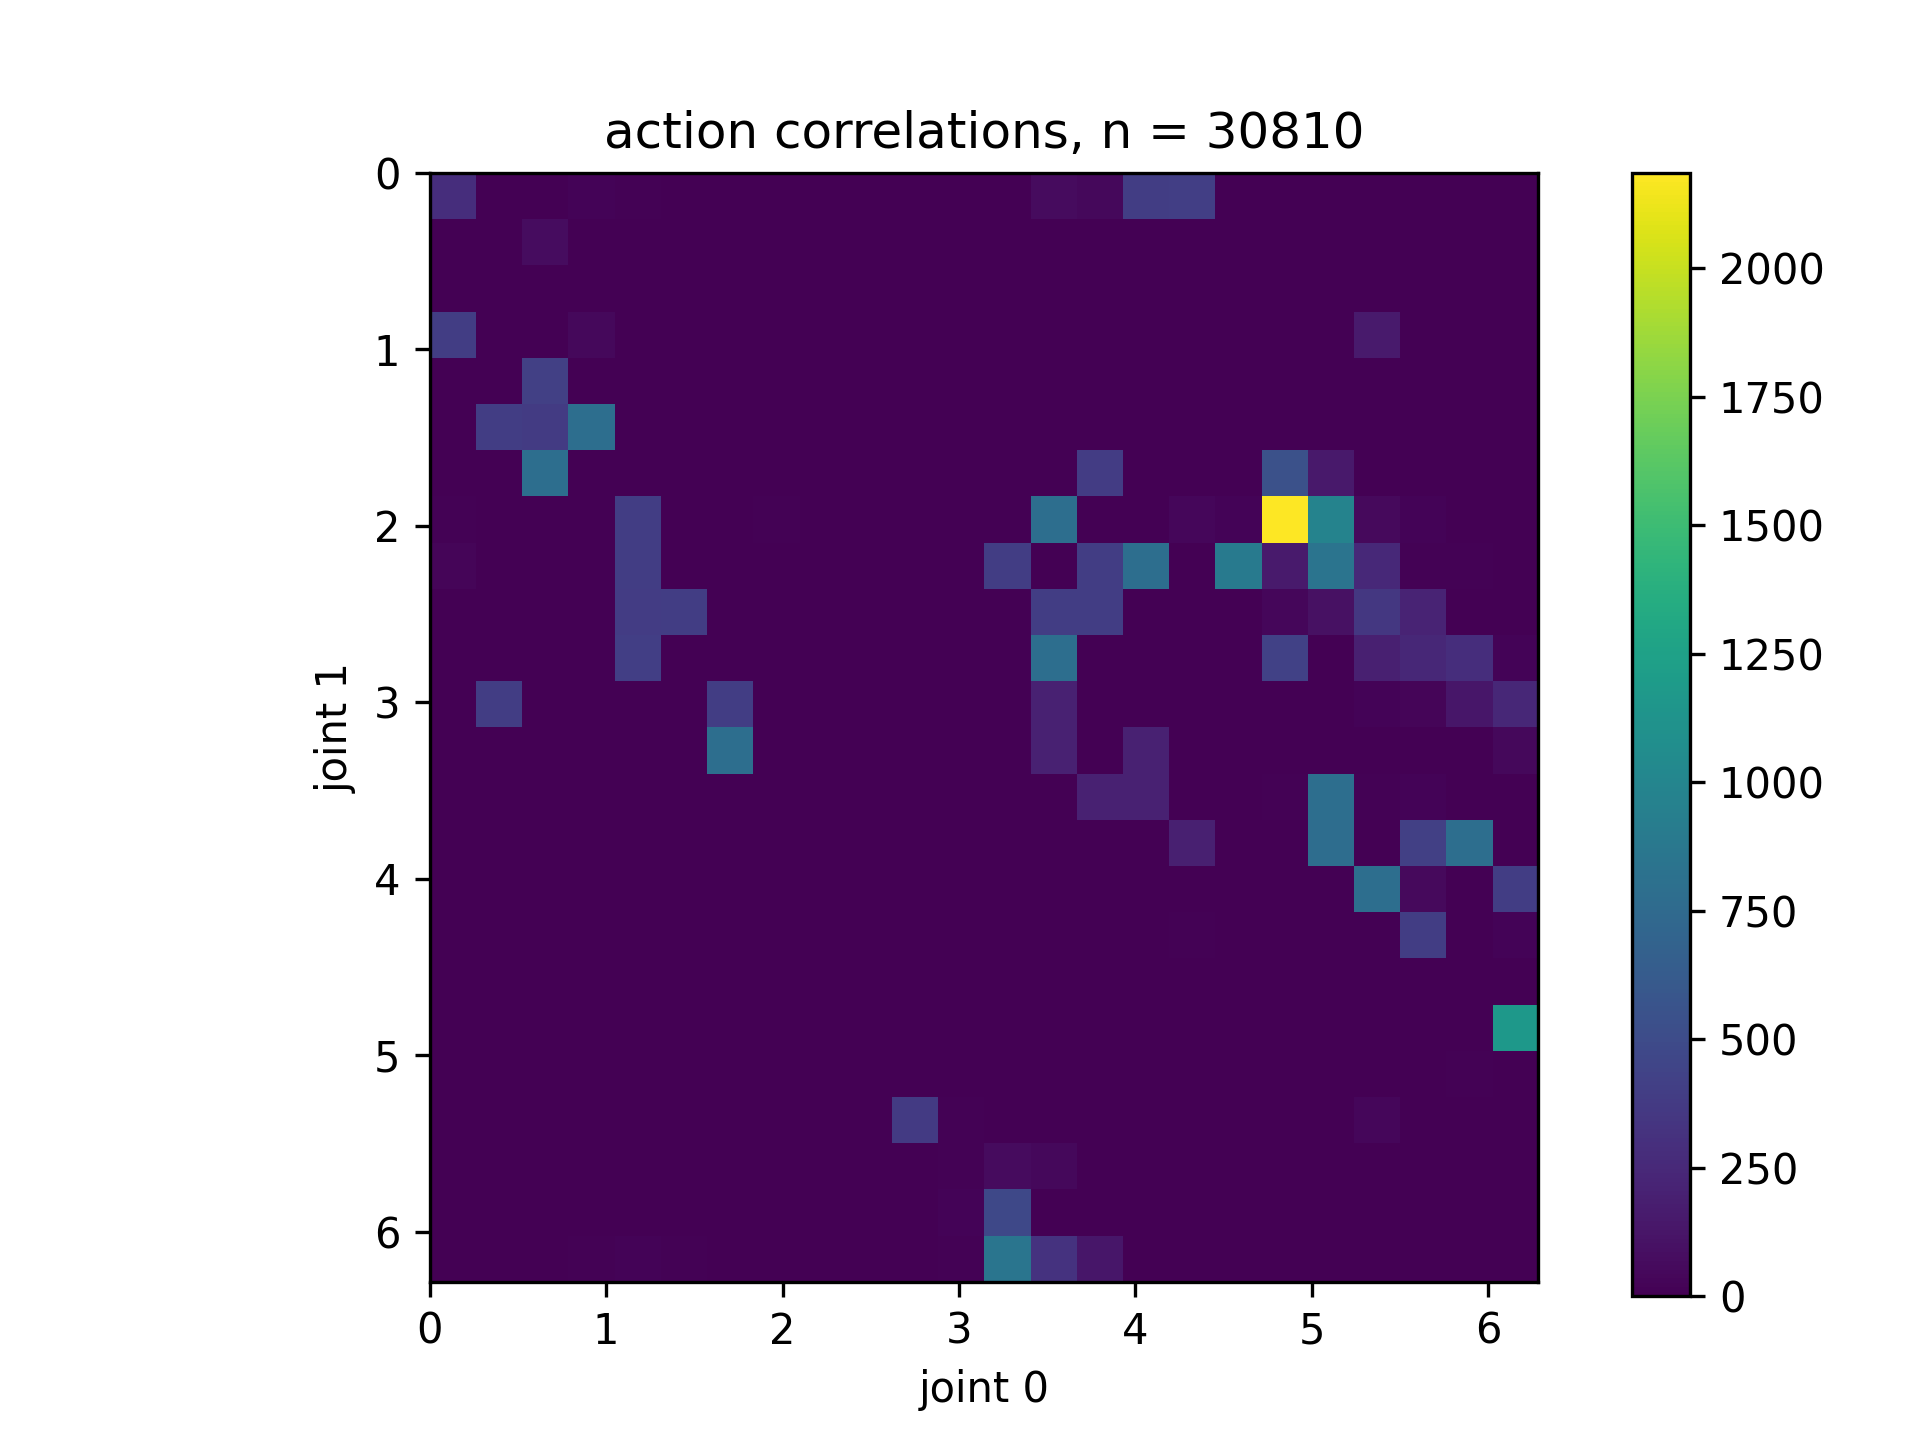
\includegraphics[width=0.23 \linewidth]{figures/experiments/action_correlations_latent_actor_4_2_1693063115_5000.png}
            \label{fig:SAC_action_correlation/latent_4}
            }
        \hfill
        \subfloat[laten dimension is 8. number of samples = 33247]{
            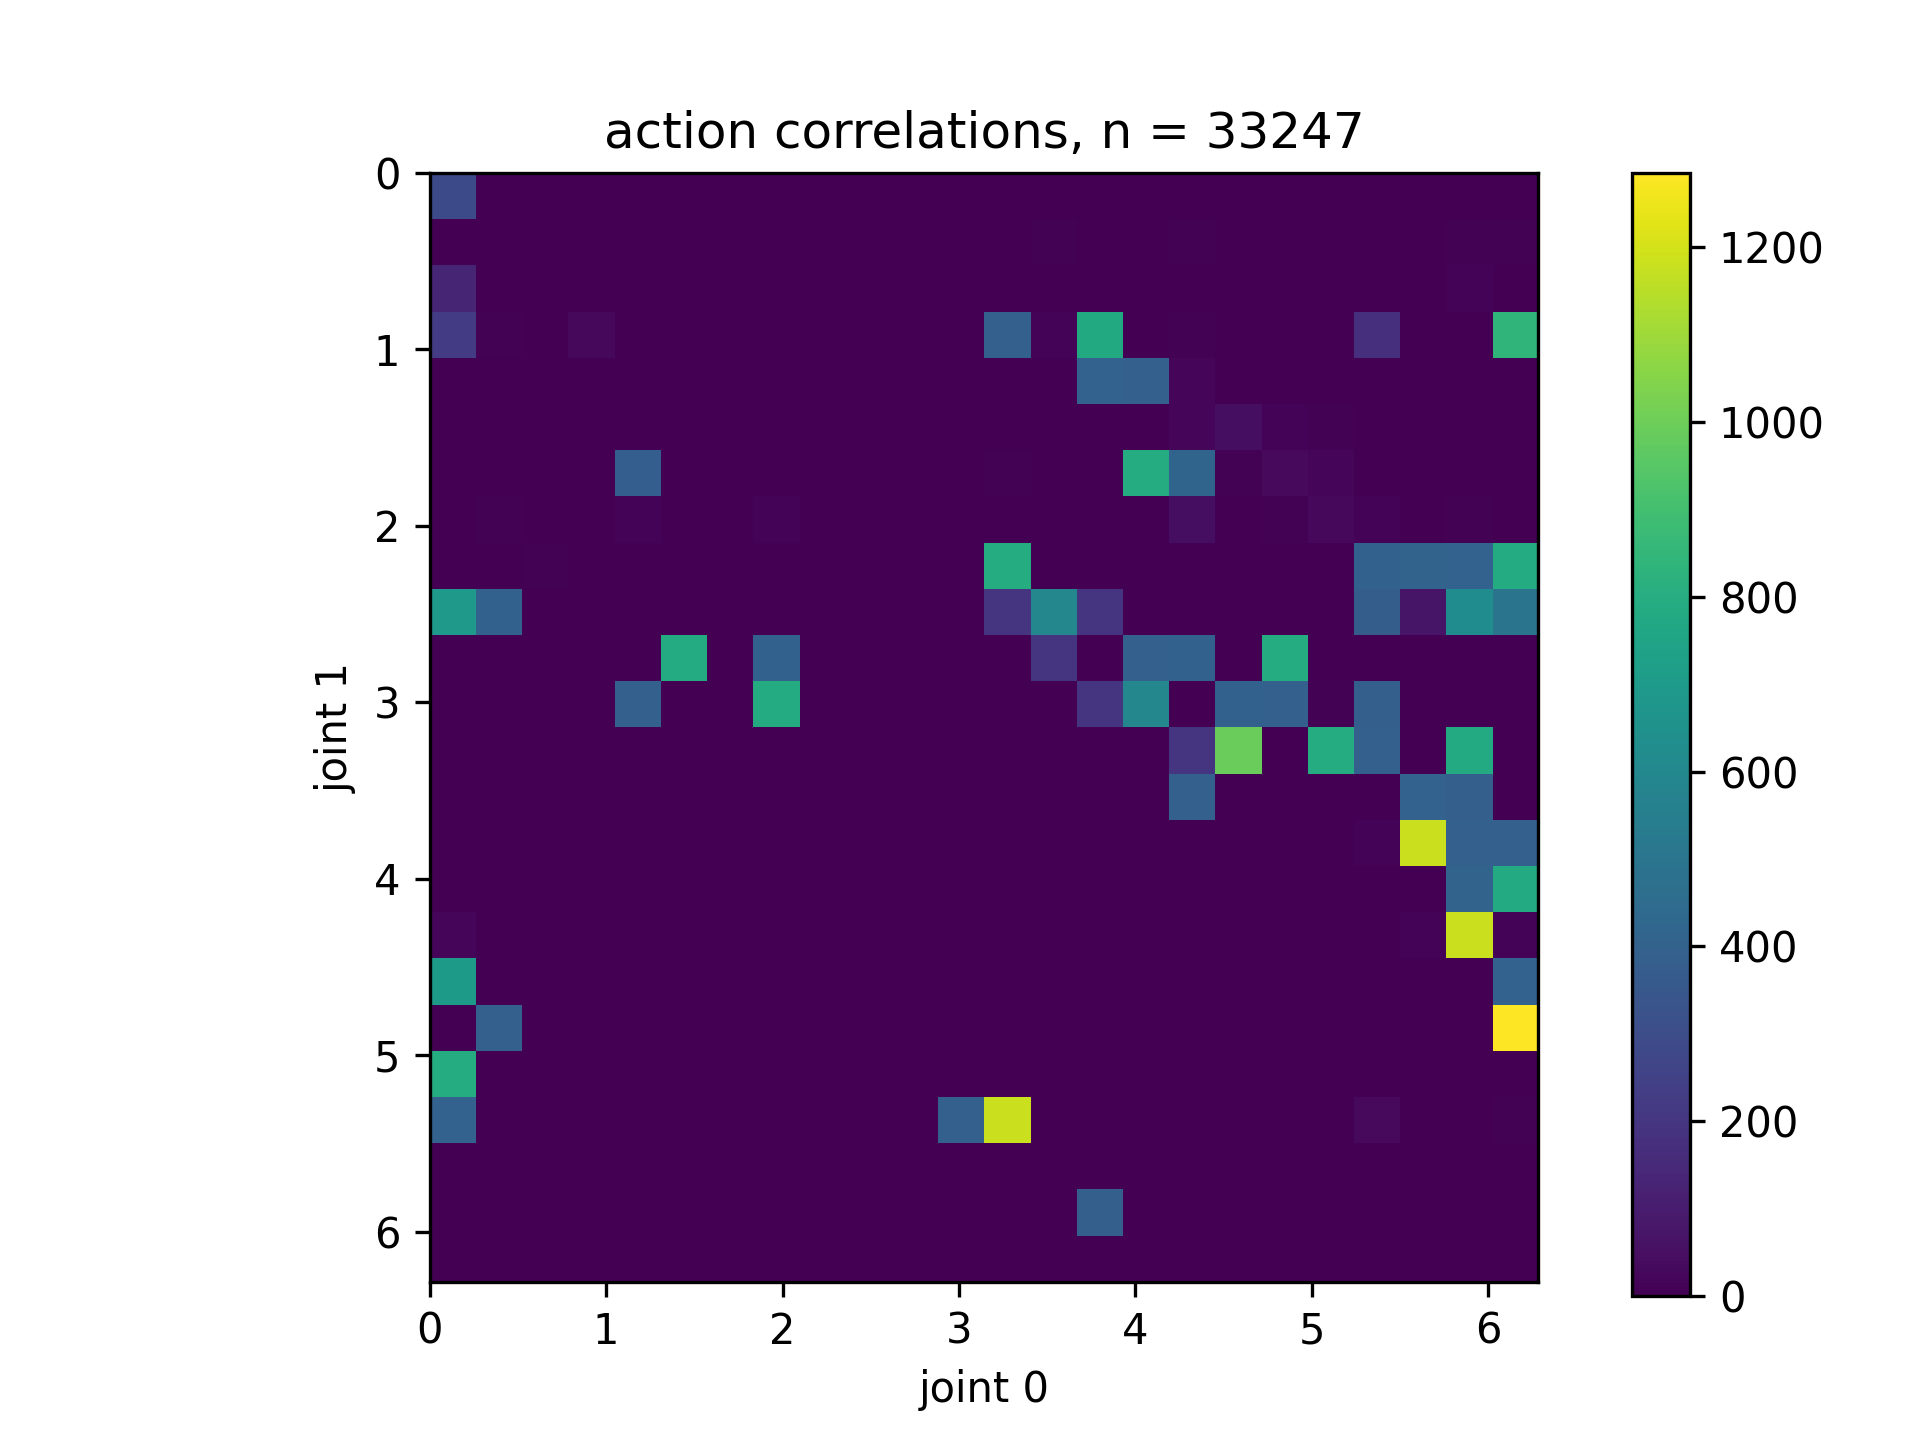
\includegraphics[width=0.23 \linewidth]{figures/experiments/action_correlations_latent_actor_8_2_1691615359_3000.png}
            \label{fig:SAC_action_correlation/latent_8}
            }
    \end{center}
    \caption[action correlation]{Plotted is the state angle correlation of two joints as a 2D histogram. The state angles are sampled from multiple episodes to uniformly sampled target positions. Each bucket can be translated to the number of angles in one 3D bucket $b$ with limits $b_{0, 0}, b_{0, 1}, b_{1, 0}, b_{1, 1}$. Mathematical speaking: $|b| = |\{q_t | q_t \in [0, 2\pi)^2 \land q_{0, t} \in [b_{0, 0}, b_{0, 1}] \land q_{1, t} \in [b_{1, 0}, b_{1, 1}]\}|$}
    \label{fig:SAC_action_correlation}
\end{figure}

\begin{table}
    \begin{center}
        \begin{tabular}{ l l | l l l l l}
        experiment series           & $N$                   & 2    & 5    & 10   & 15   & 20   \\
        \hline
        \hline
        \textit{baseline}           & $\mathfrak{S}$        & 0.73 & 0.83 & 0.57 & 0.42 & 0.30 \\
                                    & max eval $\bar{R_t}$  & 0.09 & 0.10 & 0.32 & 0.74 & 0.82 \\
        \hline
        \textit{latent 2}           & $\mathfrak{S}$        & 0.66 & 0.78 & 0.33 & 0.04 &      \\
                                    & max eval $\bar{R_t}$  & 0.11 & 0.15 & 0.83 & 3.62 &      \\
        \hline
        \textit{latent 4}           & $\mathfrak{S}$        & 0.76 & 0.84 & 0.54 & 0.04 &      \\
                                    & max eval $\bar{R_t}$  & 0.09 & 0.09 & 0.50 & 3.89 &      \\
        \hline
        \textit{latent 8}           & $\mathfrak{S}$        & 0.72 & 0.88 & 0.22 & 0.06 &      \\
                                    & max eval $\bar{R_t}$  & 0.09 & 0.08 & 2.97 & 4.22 &      \\
        \hline
        \textit{latent imitation}   & $\mathfrak{S}$        & 0.85 & 0.85 & 0.45 & 0.11 &      \\
                                    & max eval $\bar{R_t}$  & 0.08 & 0.10 & 0.44 & 2.01 &      \\
        \hline
        \textit{super distance}     & $\mathfrak{S}$        & 0.62 & 0.60 & 0.53 &      &      \\
                                    & max eval $\bar{R_t}$  & 0.11 & 0.20 & 0.64 &      &      \\
        \hline
        \textit{super imitation}    & $\mathfrak{S}$        & 0.19 & 0.25 & 0.21 &      &      \\
                                    & max eval $\bar{R_t}$  & 0.37 & 0.34 & 0.71 &      &      \\
    \end{tabular}
    \end{center}
    \caption[SAC Solved ratio]{Solved ratio $\mathfrak{S}$ and closest distance to target during one episode as known as the maximum reward during one episode for one target position, for all SAC experiments starting at $[N, 0]$ and targeting the same targets as in \figref{fig:SAC_baseline_min_distances} with a maximal budget of 400 steps. Those are examples from individual experiments all from epoch 3000. For more details on which experiments please have a look at the figures directory. The suffix of each png describes where to find the experiment. For a closer inspection of how the individual models perform over the evaluation please refer to \chapref{chap:appendix}}
    \label{tab:SAC_solved_ratio}
\end{table}

A comparison between CCD and baseline SAC revealed several intriguing distinctions:

\begin{itemize}
    \item \textbf{Target Dependence}: Upon closer examination of CCD, it became evident that its performance in a single run was significantly influenced by the initial configuration and the specific target location. This was well-illustrated in  \figref{fig:CCD_iteration}, which depicted CCD's performance in terms of the number of iterations required to reach the desired target position. Interestingly, when we analyzed the steps needed to reach the target position using SAC, a noteworthy trend emerged. As the number of joints increased, we found that SAC more frequently reached the maximum iteration limit rather than successfully reaching the target as illustrated in \chapref{chap:appendix} and \tabref{tab:SAC_solved_ratio}. One potential explanation, alluded to in \figref{fig:SAC_baseline_inference_trajectory}, was that the agent's behavior sometimes declined as it neared the target. After coming tantalizingly close, the end-effector would rapidly retreat towards the arms origin, failing to get as close to the desired target as before. This observation was backed up by \figref{fig:SAC_baseline_min_distance_step}, which showed that the minimum distance to the target was typically achieved in around 50 steps or fewer during an episode. It's worth noting that this difficulty in reaching the target could be attributed to SAC's fixed threshold for ending an episode, which required a $0.1$ Euclidean distance between the end-effector and the target by definition. As the number of joints increased, the area within which the end-effector's position could end an episode diminished quadratically, making it progressively harder to reach the target with more joints. However, this argument was counterbalanced by the fact that the robot arm could execute more precise movements or potentially decompose the problem into smaller parts. For instance, joint $1$ to $N-2$ could be utilized to roughly position the end-effector near the target, while joint $N-1$ to $N$ could perform the precise adjustments. This raises a crucial question: why did the agent consistently fail, often by a substantial margin, after coming so close to the target? One plausible explanation is that the agent frequently encountered scenarios where it almost reached the target but had no opportunity to learn from these experiences. On the contrary, the extended episode length and increasing failure rate while increasing $N$, as seen in  \tabref{tab:SAC_solved_ratio}, should work against this trend.
    \item \textbf{Solutions}: A deeper exploration of how SAC and CCD tackled inverse kinematics problems unveiled a strong contrast in the distribution of state angles. Comparing \figref{fig:dataset_action_correlation}, which depicted the state angle distribution required to reach the target in the dataset, with \figref{fig:SAC_action_correlation/baseline}, which illustrated the distribution resulting from baseline SAC, highlighted this discrepancy. While the former exhibited a rhombus-shaped distribution, the latter showcased a more scattered pattern.
\end{itemize}

It is important to recognize that this qualitative comparison between CCD and SAC is inherently limited. CCD enjoys unrestricted access to the entire action space, whereas SAC's action range is constrained due to action normalization. It's also noteworthy that scaling the hyperbolic tangent output to a range of $2\pi$ or higher, while a potential solution, is not without its challenges. Doing so could lead to SAC finding multiple actions that yield the same action outcome or potentially complicate the calculation of log probabilities for the policy.

At this juncture, we can draw connections between our baseline experiments and the concepts presented in the Motor Synergy paper \cite{Motor_Synergy_Learning}. An interesting proposition arises when we closely examine the inverse kinematics problem as defined in the environment description. One conceivable strategy involves dividing the robot arm into two sections, each comprising $N/2$ segments, and constraining the relative angles within each segment. These two segments would effectively resemble a robot arm with just two extended joints. As previously demonstrated, environments with two joints are quite tractable. Yet, why doesn't the policy opt for such a strategy? Several arguments come to the fore. It's plausible that this strategy results in a longer trajectory to reach the target, which could affect the accumulated reward. Additionally, the choice could be influenced by the exploration strategy, as increasing entropy to encourage exploration does not seem effective due to the collapsing distribution, as seen in \figref{fig:Uniform_dataset}.

The decrease in SAC's performance, as evidenced in \figref{fig:SAC_baseline}, can also be attributed to the linear growth in the complexity of the observation space, given that $S$ is a subset of $\mathbb{R}^{4+N}$. To address this escalating complexity, researchers might consider increasing the number of hidden layers or neurons per layer while delving into neural architecture search. An alternative approach for investigating this theory could involve the application of Neural-Evolution-of-Augmented-Topologies (NEAT). This algorithm seeks to identify the smallest neural architecture capable of solving a given task. Given the context provided, it's reasonable to assume that the discovered neural architecture becomes increasingly complex as $N$ increases.




\begin{figure}
    \begin{center}
        \subfloat[$N = 2$]{
            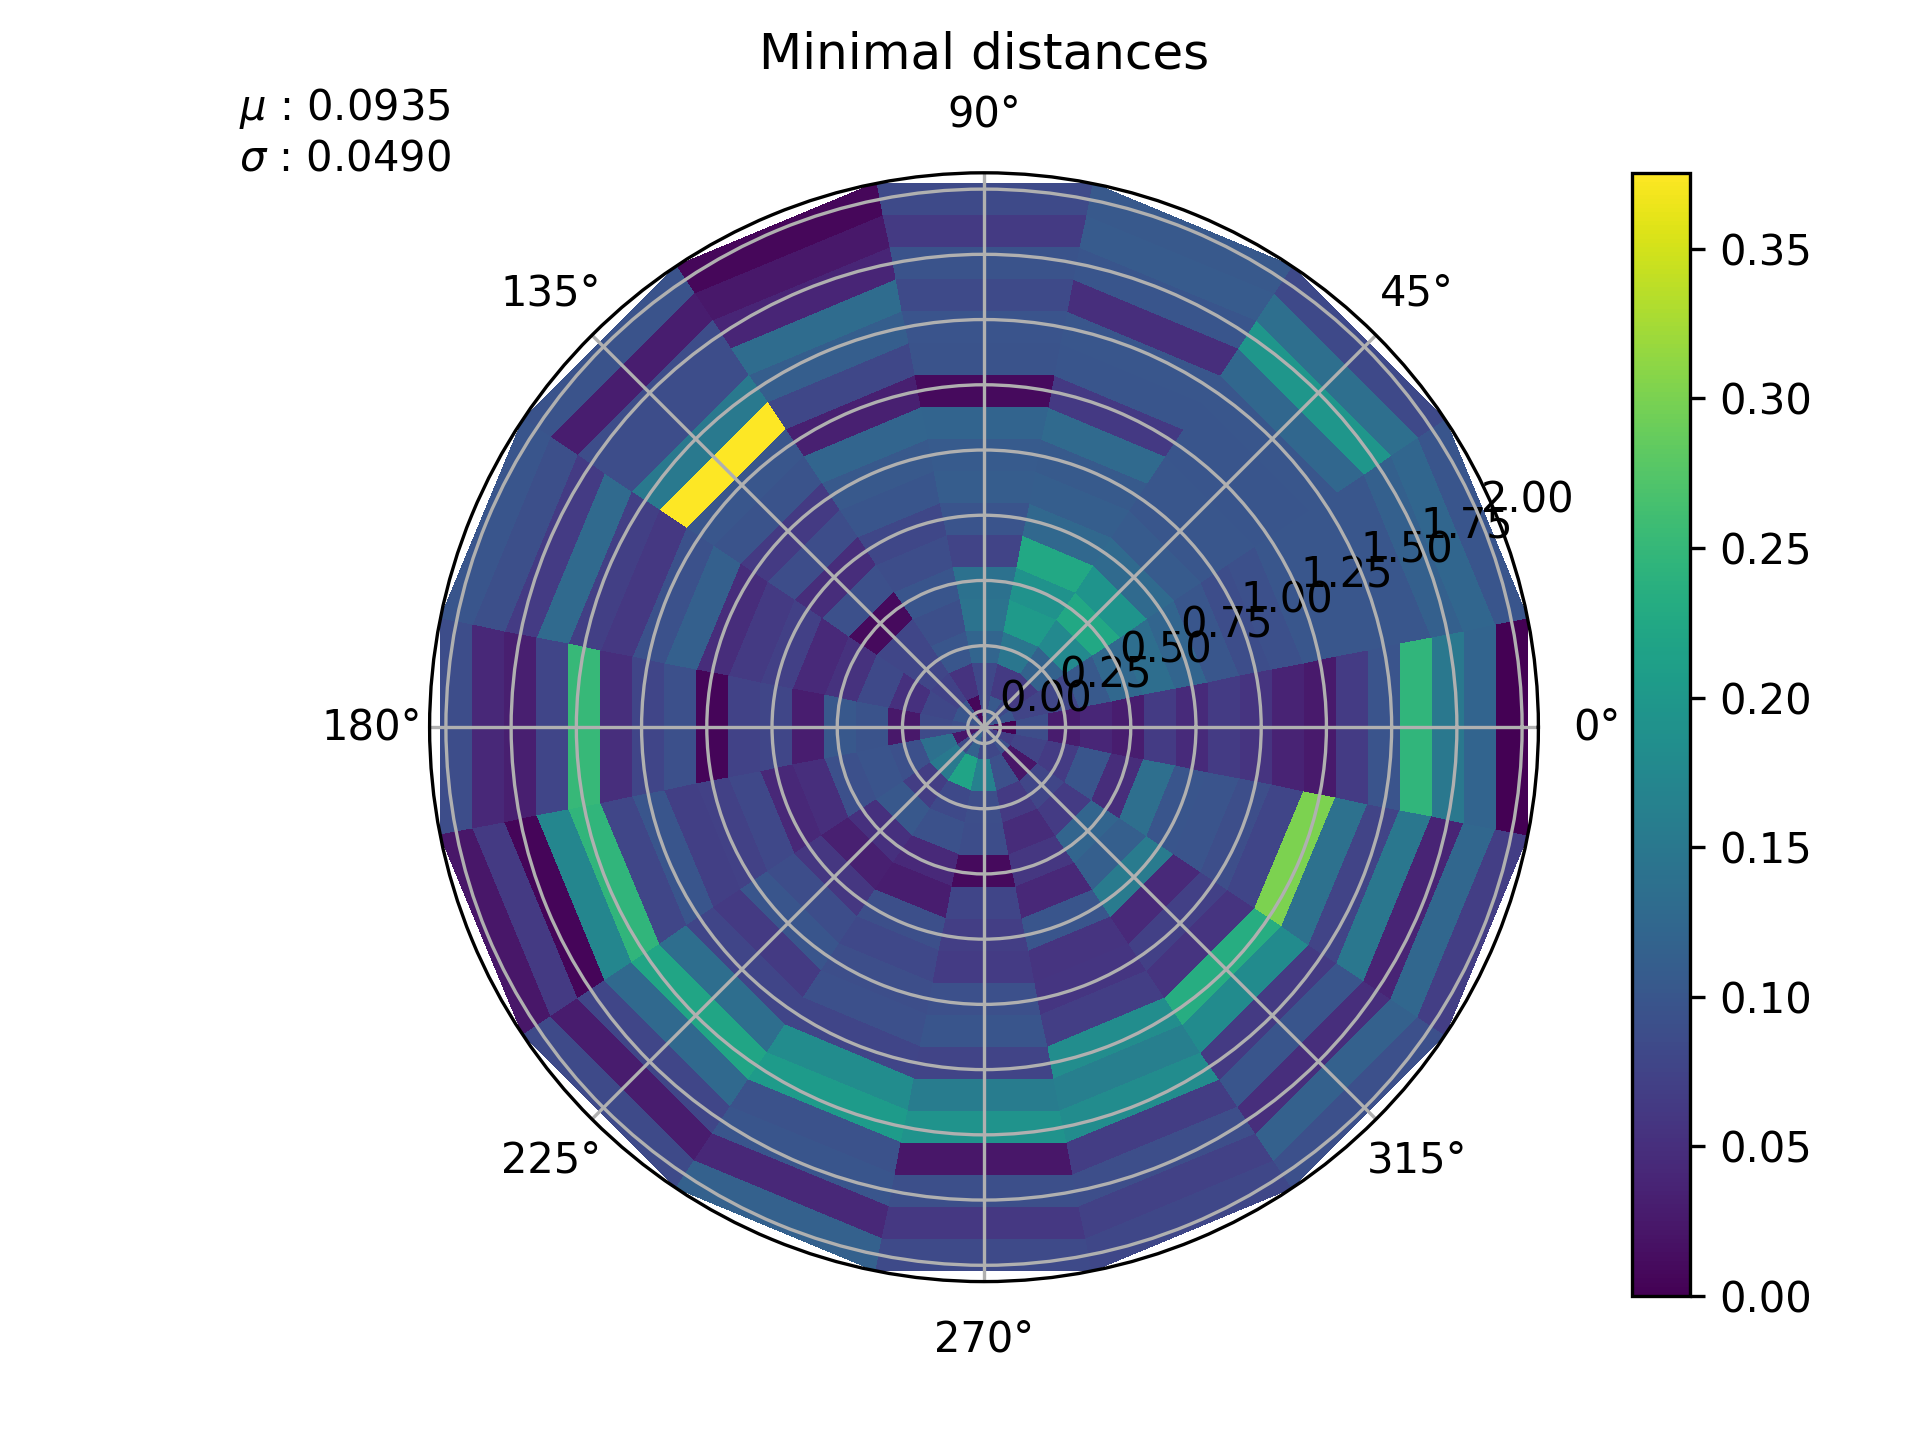
\includegraphics[width=0.31 \linewidth]{figures/experiments/Minimal_distances_baseline_2_1691621262_5000.png}
            \label{fig:SAC_baseline_min_distances/2}
            }
        \hfill
        \subfloat[$N = 5$]{
            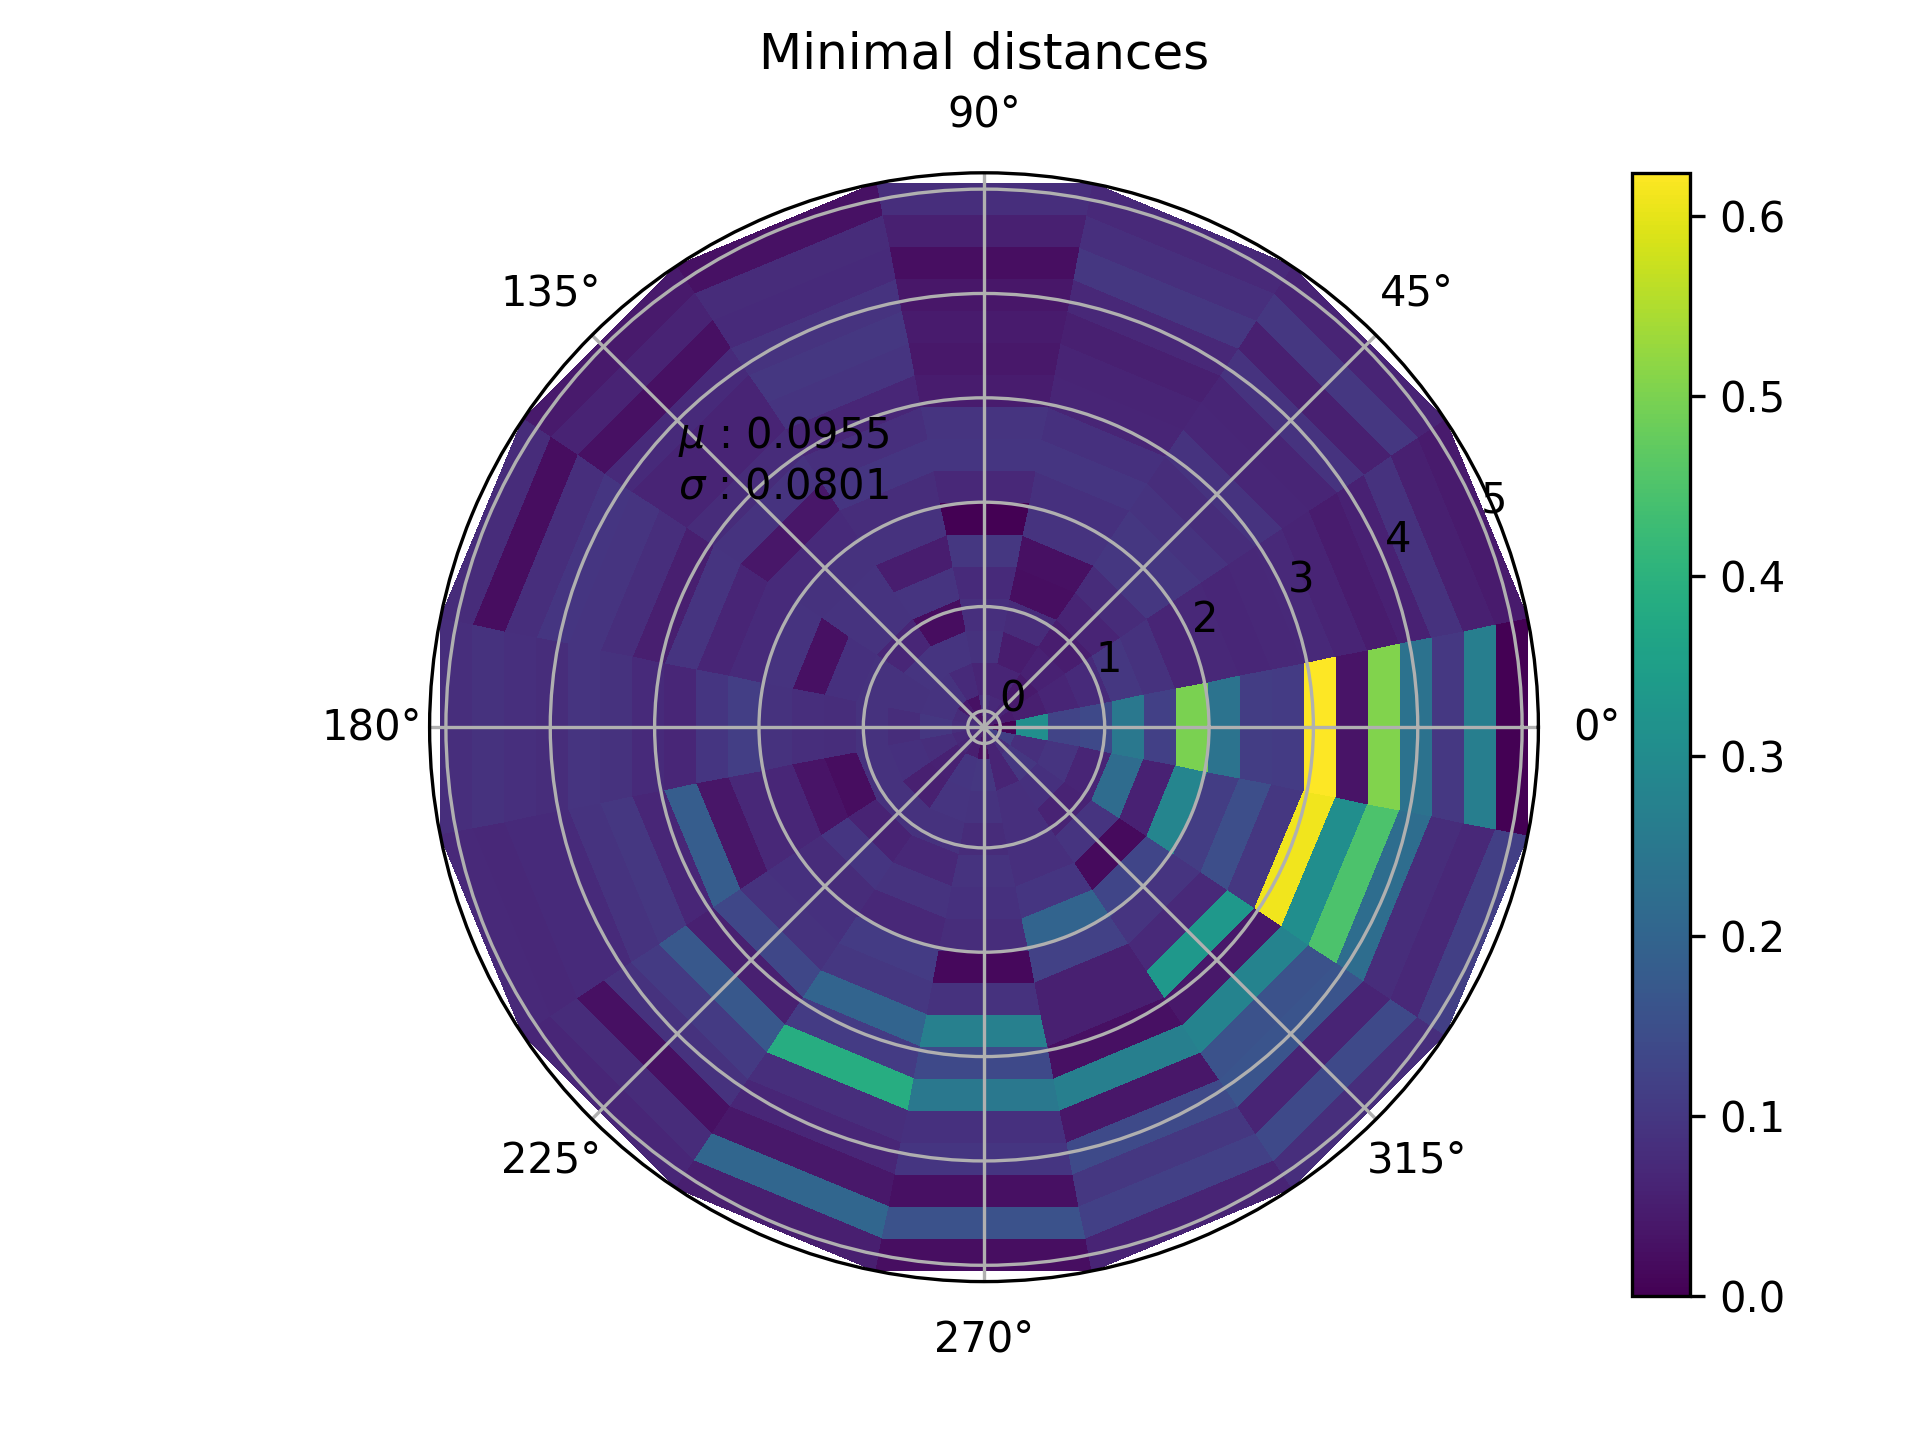
\includegraphics[width=0.31 \linewidth]{figures/experiments/Minimal_distances_baseline_5_1691621331_5000.png}
            \label{fig:SAC_baseline_min_distances/5}
            }
        \hfill
        \subfloat[$N = 10$]{
            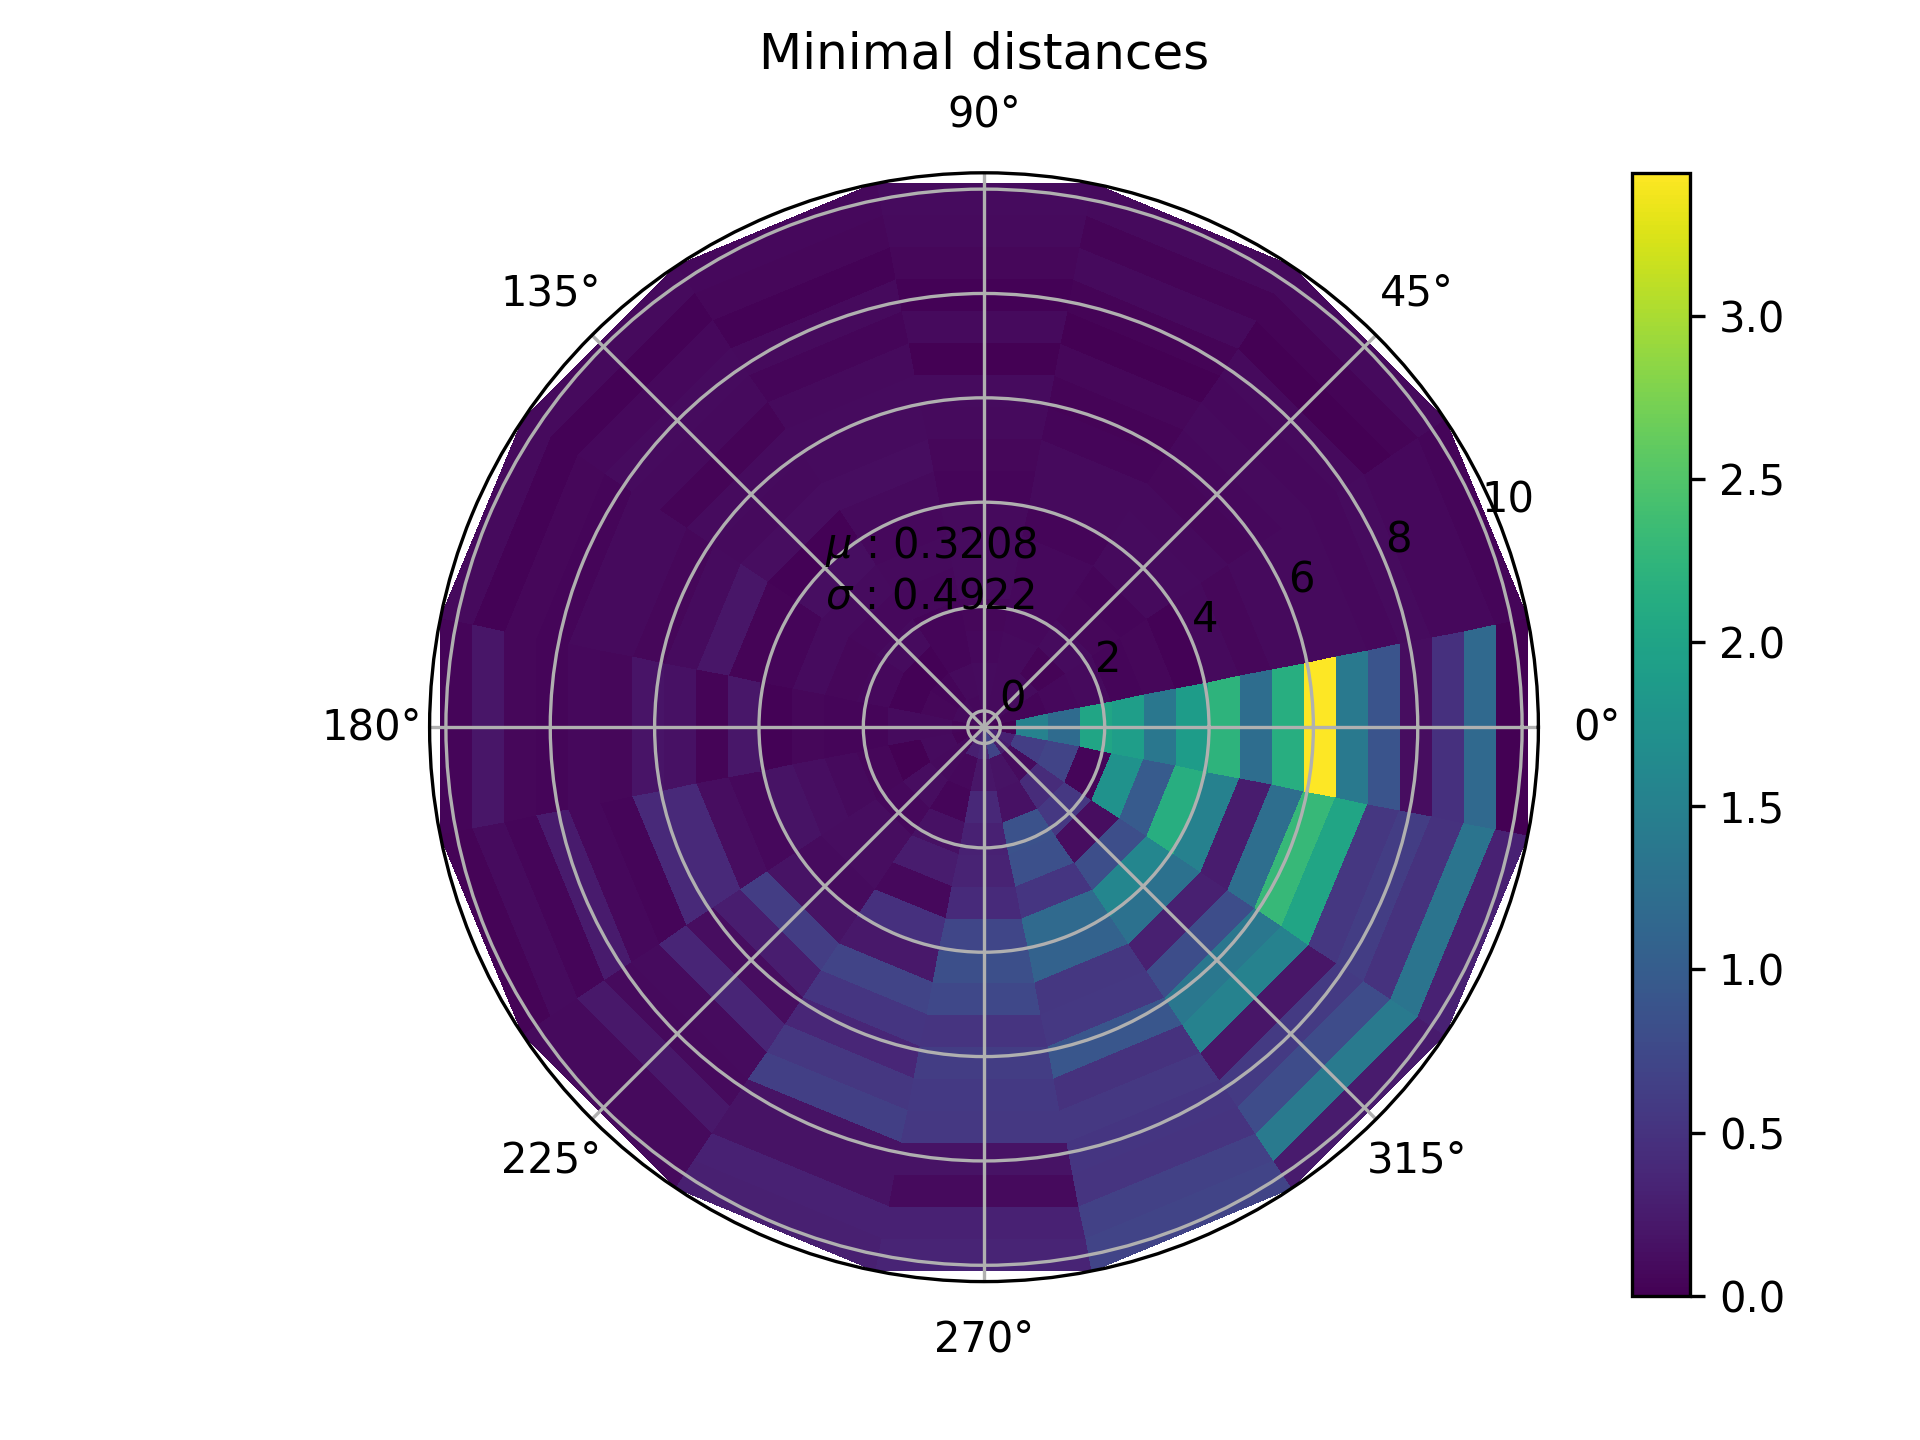
\includegraphics[width=0.31 \linewidth]{figures/experiments/Minimal_distances_baseline_10_1691618968_5000.png}
            \label{fig:SAC_baseline_min_distances/10}
            }
    \end{center}
    \caption[SAC min distance heatmap]{Minimal distance to a target during inference starting from $[N , 0]$ and targeting the middle of each polygon.}
    \label{fig:SAC_baseline_min_distances}
\end{figure}


\begin{figure}
    \begin{center}
        \subfloat[$N = 2$]{
            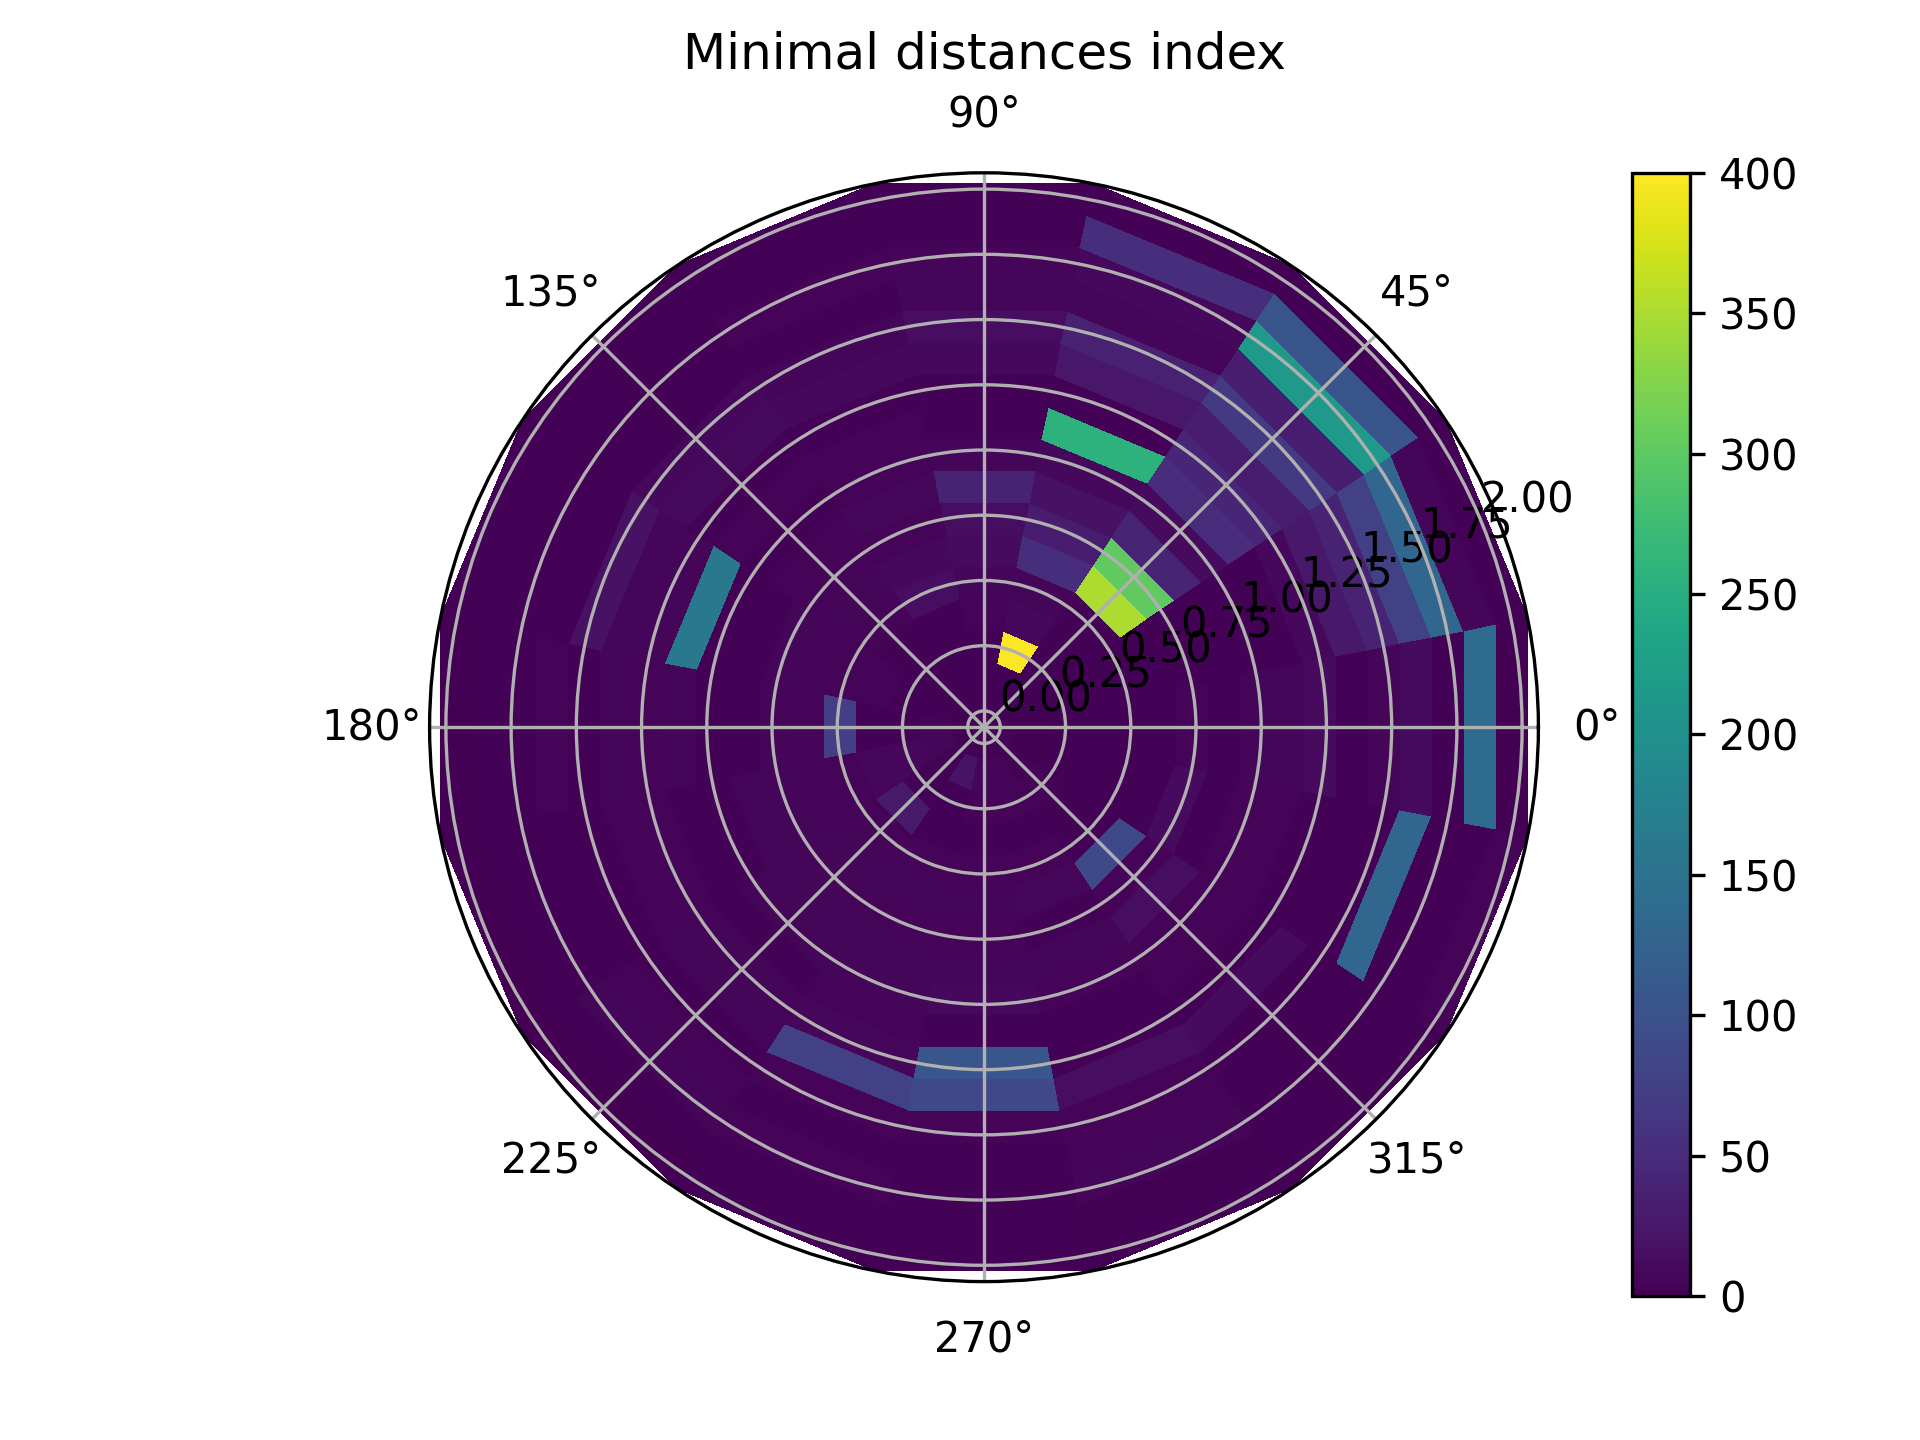
\includegraphics[width=0.31 \linewidth]{figures/experiments/Minimal_distances_index_baseline_2_1691621262_5000.png}
            \label{fig:SAC_baseline_min_distance_step/2}
            }
        \hfill
        \subfloat[$N = 5$]{
            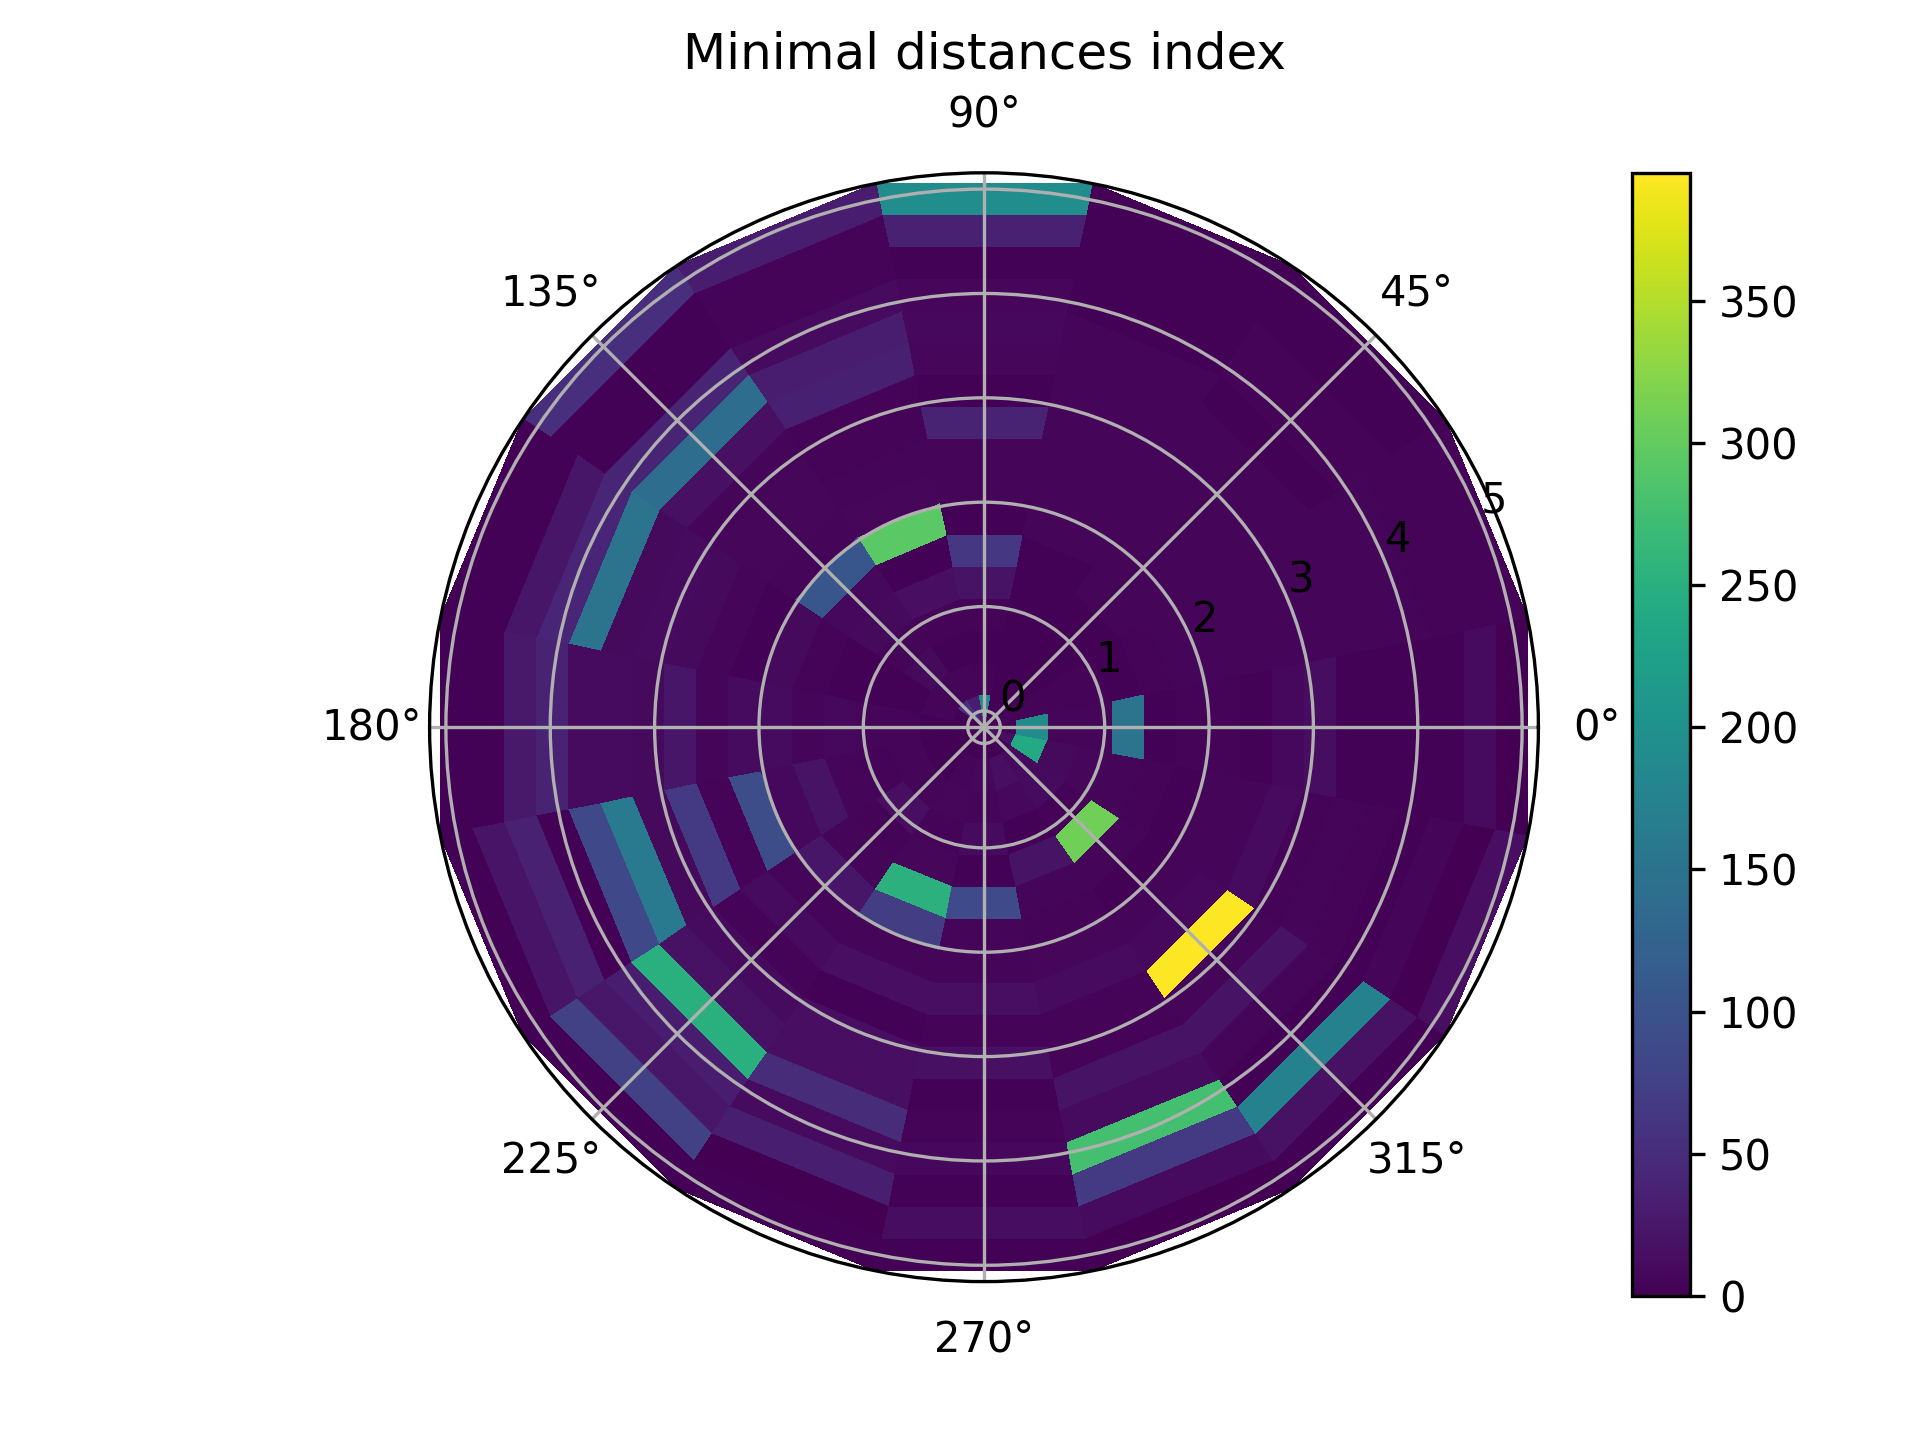
\includegraphics[width=0.31 \linewidth]{figures/experiments/Minimal_distances_index_baseline_5_1691621331_5000.png}
            \label{fig:SAC_baseline_min_distance_step/5}
            }
        \hfill
        \subfloat[$N = 10$]{
            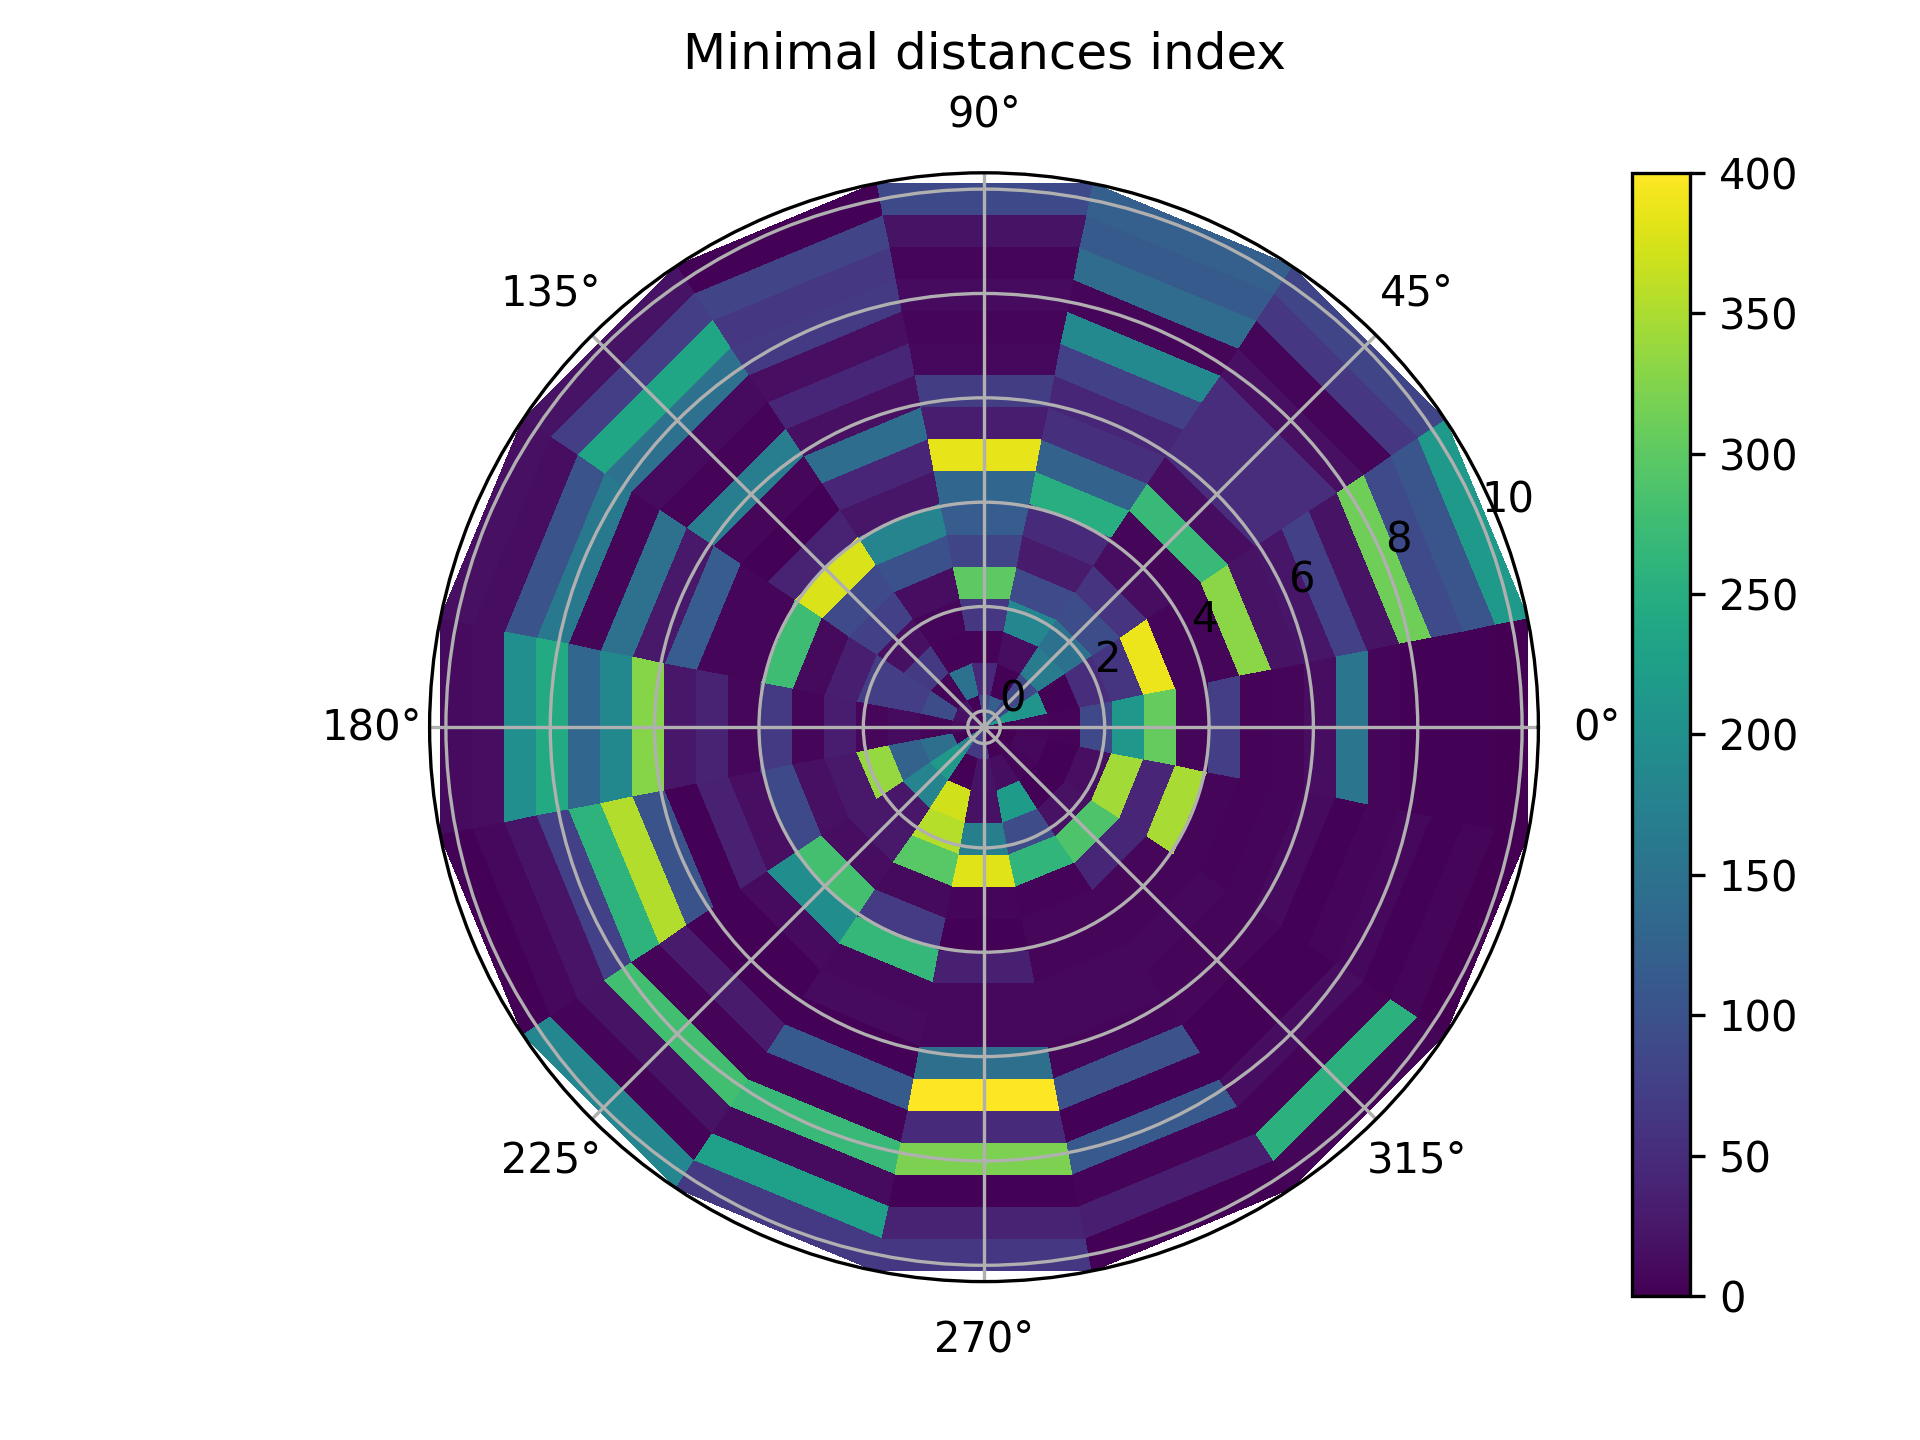
\includegraphics[width=0.31 \linewidth]{figures/experiments/Minimal_distances_index_baseline_10_1691618968_5000.png}
            \label{fig:SAC_baseline_min_distance_step/10}
            }
    \end{center}
    \caption[SAC iteration heatmap]{Heatmap of how many iterations baseline SAC has needed to solve inverse kinematics starting from $[N, 0]$ targeting the middle of each polygon. The maximum budget is 20 times $N$ with a target precision of $0.1$.}
    \label{fig:SAC_baseline_min_distance_step}
\end{figure}

\section{SAC with Latent Model}

The integration of the Latent Model into the SAC framework yielded the results showcased in \chapref{chap:experiments}. While comprehending the striking disparities in problem-solving strategies between the trained latent models, as illustrated in \figref{fig:SAC_action_correlation}, and the Inverse Kinematics solver CCD, as depicted in \figref{fig:dataset_action_correlation}, it is rather astonishing that this approach was effective. Typically, such a substantial shift in the distribution of the observation space would result in unpredictable and unworkable behavior in the predicted actions within the Action space. We attempted to address this challenge by introducing the imitation loss, emphasizing predicted actions that led to state angles much closer to the original distribution.

As seen earlier, we obtained varying performances from the VAEs with different latent dimensions. But why? Let's first consider the experiments with a latent dimension of two. Given that we are endeavoring to encode two-dimensional target information, which is sampled by the concept of the \texttt{TargetGaussianDataset}, into a two-dimensional Gaussian manifold, the most efficient strategy for retaining information would involve channeling the mean values while returning a standard deviation close to zero. Since we employ the Evidence Lower Bound (ELBO) with a Gaussian distribution for a Variational Autoencoder (VAE), we must select a parameterized latent distribution that closely approximates the standard normal distribution. An additional challenge lies in encoding the target position as independent random variables. Given these properties and constraints, compressing this information can indeed be quite challenging. On the other hand, selecting a latent dimension that is too high can introduce excessive computational complexity, sampling difficulties, and a reduction in robustness.

Based on these observations, we propose setting the latent dimension of a VAE as an additional hyperparameter to optimize. Setting it too high can result in the extremely high variance observed in the Soft Actor-Critic task, while setting it too low may lead to a loss of encoded information.

Furthermore, let's revisit the action correlation plots. As previously mentioned, these plots across all SAC experiments deviate significantly from the initial distribution, as depicted in \figref{fig:dataset_action_correlation}. However, they exhibit remarkable similarity among themselves, as illustrated in \figref{fig:SAC_action_correlation}. This is an unexpected outcome, as each model could adopt a distinct problem-solving strategy and start anew in each iteration. Conversely, activating the imitation loss in the VAE experiments and integrating this approach with SAC should ideally result in a substantial shift towards the rhombus-shaped distribution observed in Figure 5.4. However, the familiar hotspots seen in \figref{fig:dataset_action_correlation} vanish, and a new distribution emerges, characterized by the same spike at $(\pi, 0)$, as depicted in \figref{fig:SAC_action_correlation_comp/latent_4_imitation}.

% \begin{figure}[h]
%     \begin{center}
%         \subfloat[SAC baseline experiments]{
%             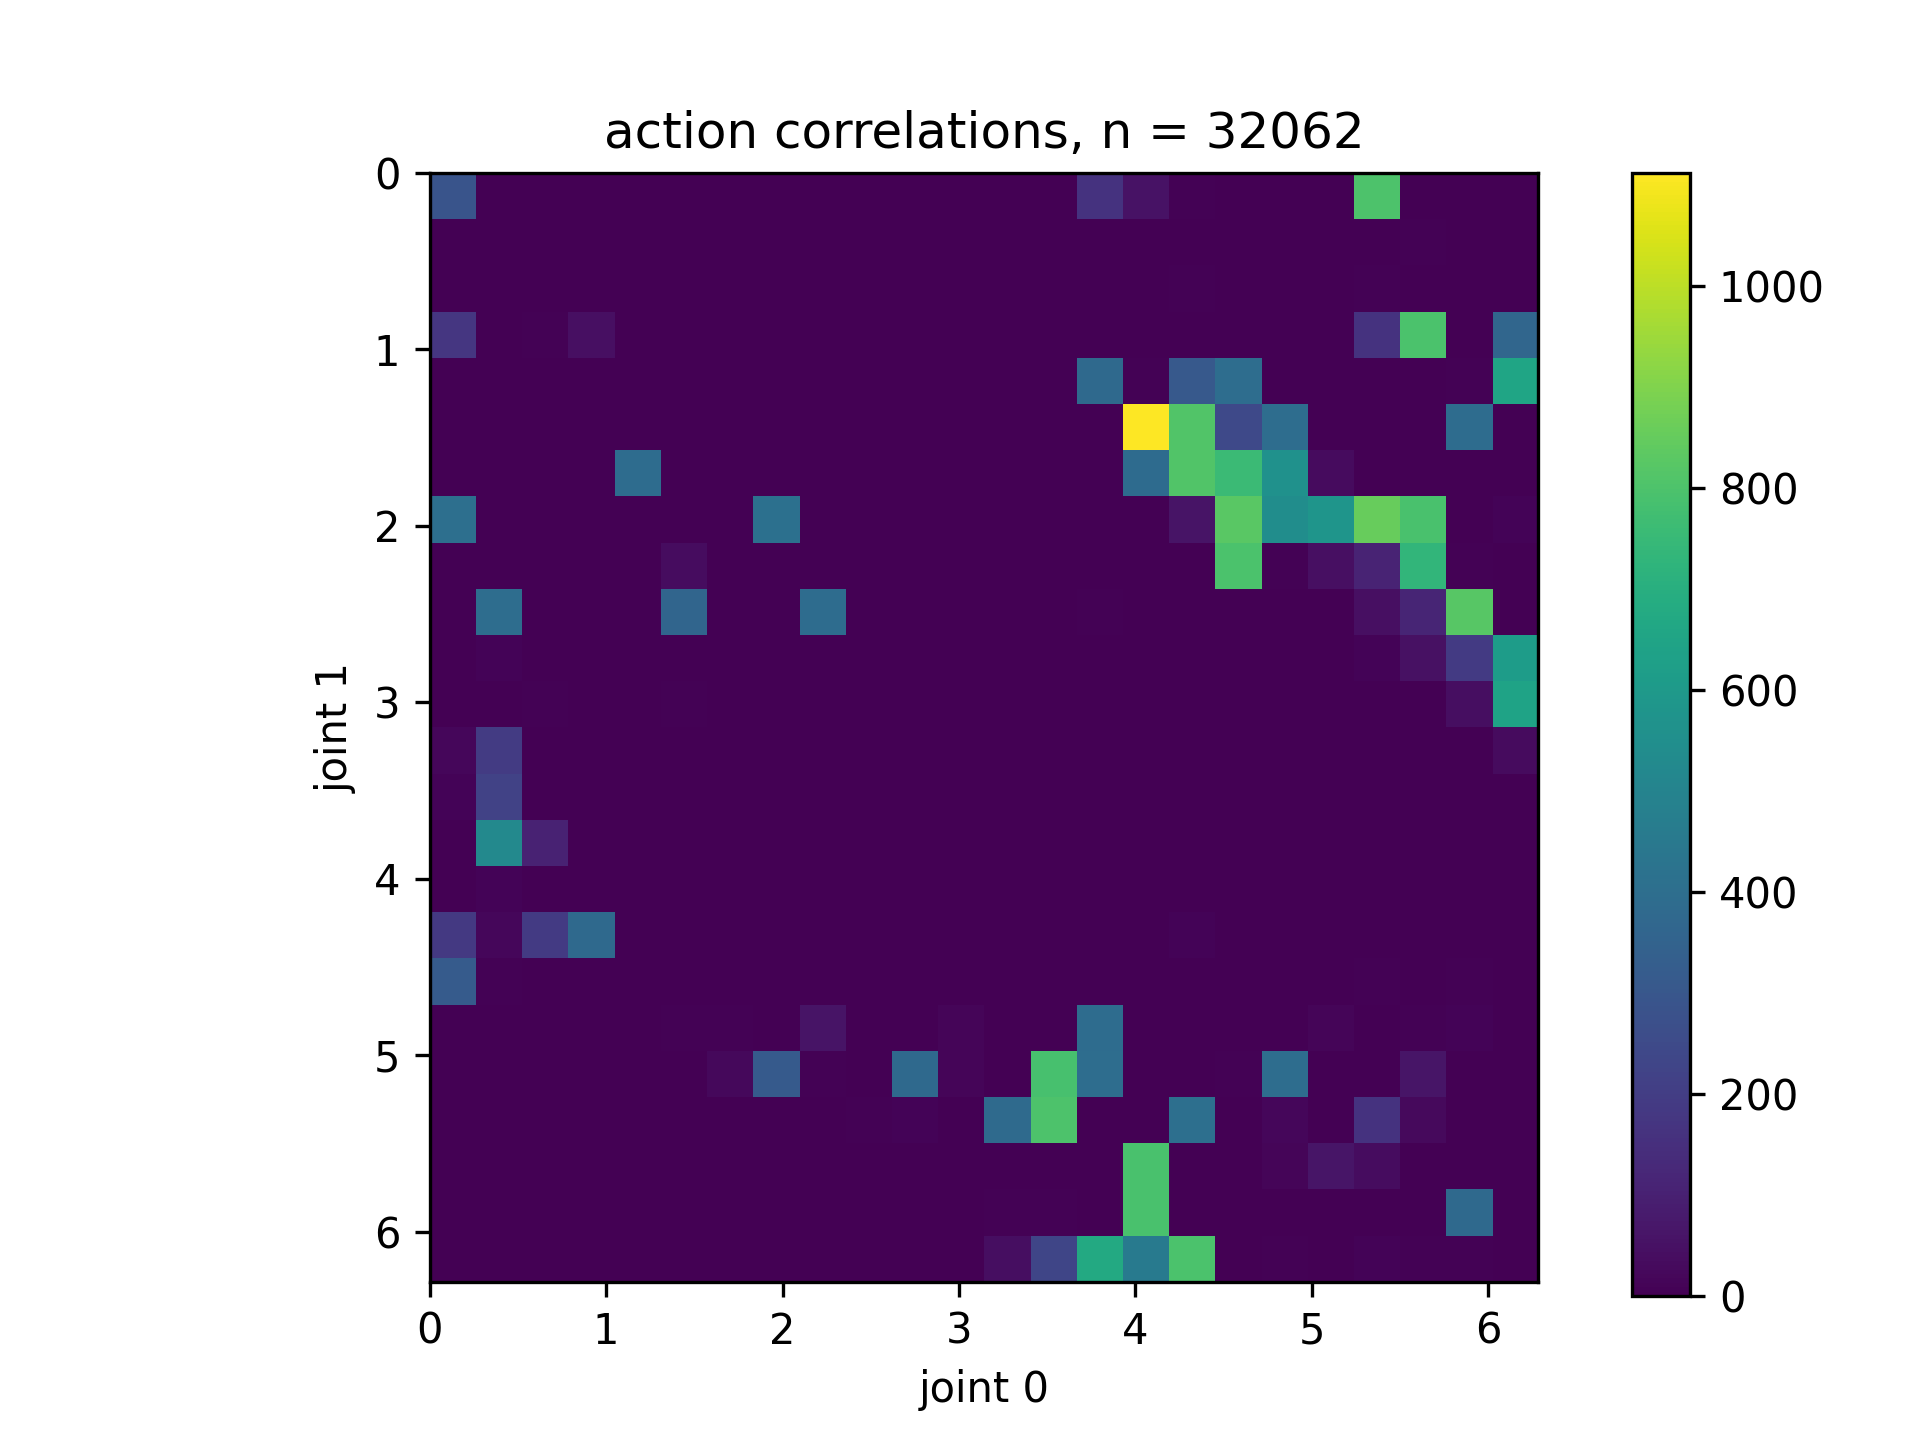
\includegraphics[width=0.31 \linewidth]{figures/experiments/action_correlations_baseline_2_1691621262_5000.png}
%             \label{fig:SAC_action_correlation_supervised/baseline}
%             }
%         \hfill
%         \subfloat[SAC + Supervised model trained only with distance loss enabled]{
%             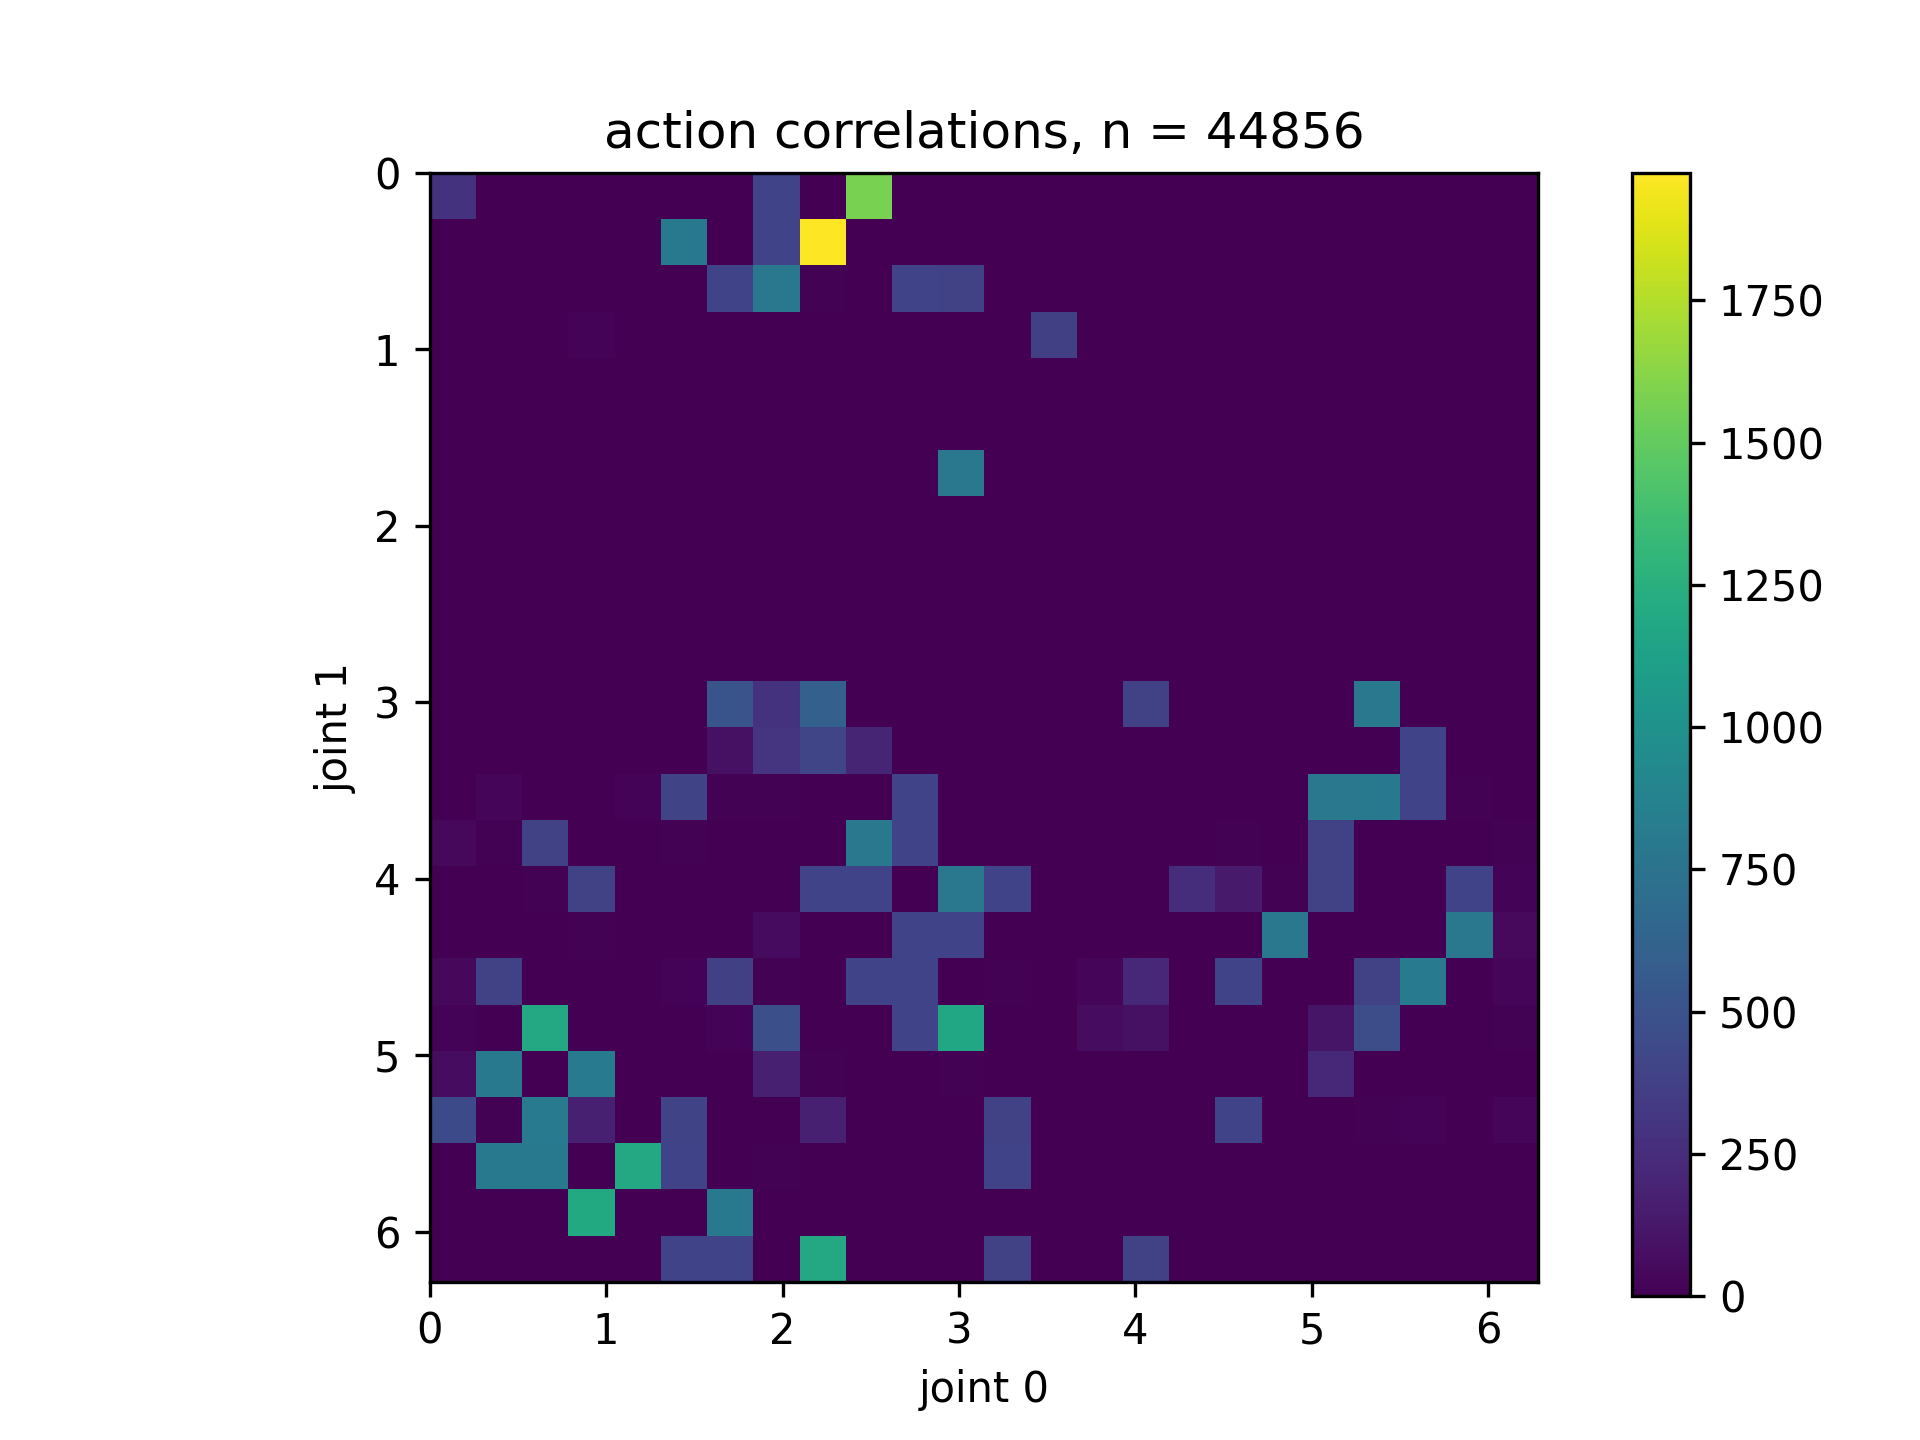
\includegraphics[width=0.31 \linewidth]{figures/experiments/action_correlations_supervised_dist_loss_2_1693272467_3000.png}
%             \label{fig:SAC_action_correlation_supervised/supervised}
%             }
%         \subfloat[SAC + Supervised model trained only with distance and imitation loss enabled]{
%             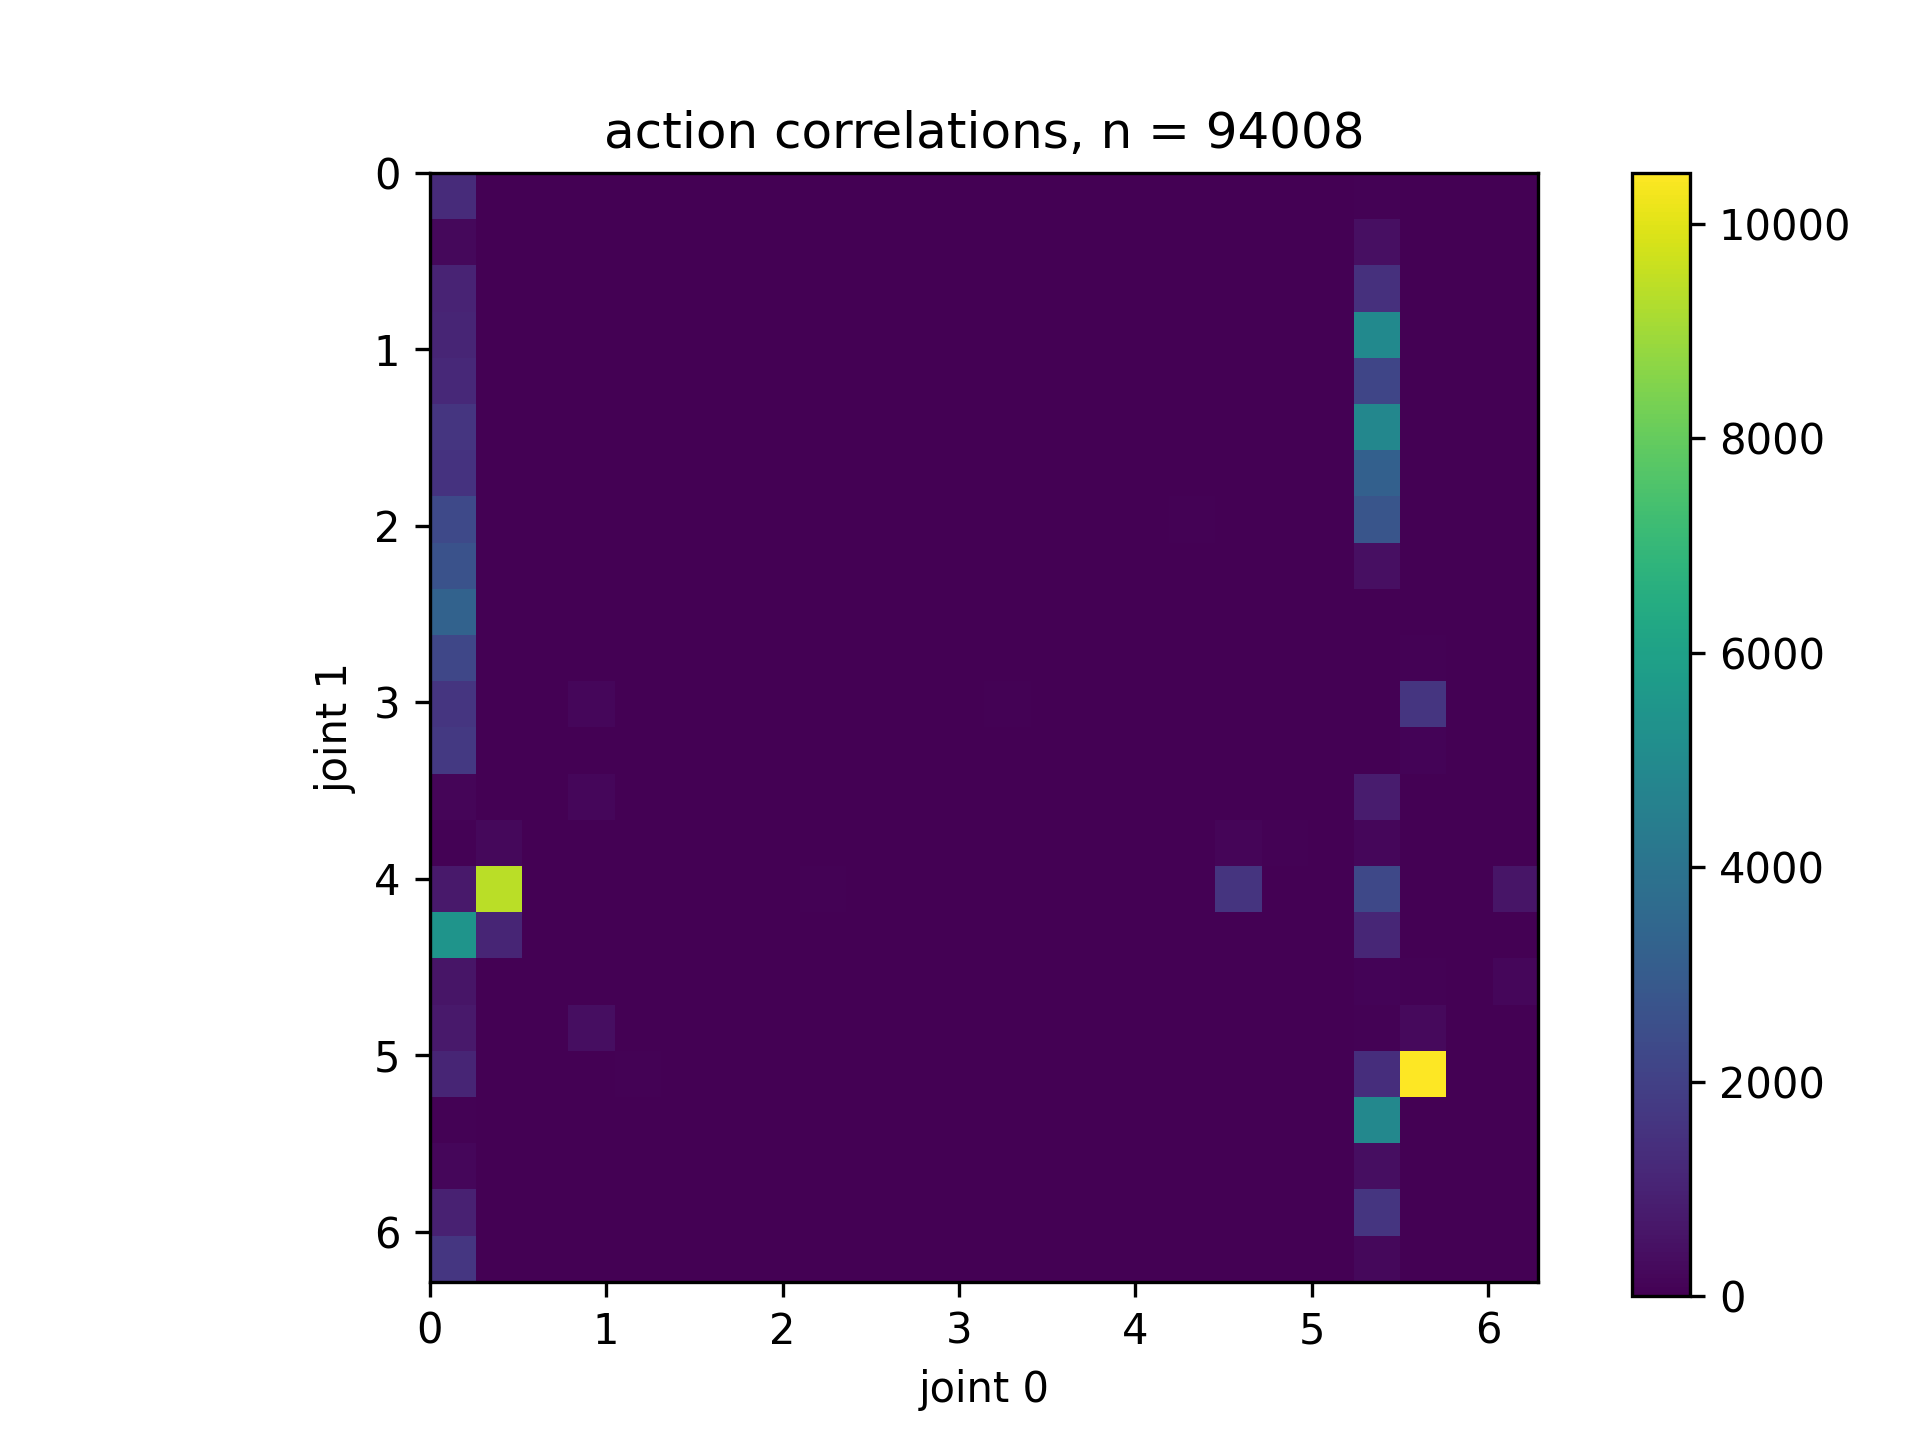
\includegraphics[width=0.31 \linewidth]{figures/experiments/action_correlations_supervised_imitation_2_1693487256_3000.png}
%             \label{fig:SAC_action_correlation_supervised/supervised_imitation}
%             }
%     \end{center}
%     \caption[action correlation comparison with supervised model]{Action correlation for baseline experiments, experiments with SAC and supervised model with only distance loss enabled and SAC with supervised model with distance and imitation loss enabled.}
%     \label{fig:SAC_action_correlation_supervised}
% \end{figure}


Finally, we want to discuss which kind of latent model someone should prefer. The VAE or the supervised learning model? \\
As we have seen in the experimental part but also in \tabref{tab:SAC_solved_ratio}, the SAC + VAE returns much more stable results and also better results compared to the supervised model. One reason might be the generalization within the training of a VAE. This results in a much smoother latent space than we could achieve with the supervised model. Another advantage of the VAE is the implied dimensionality invariance we achieve with a constant latent dimension but a different prediction dimension. An indication for this theory can seen by the almost constant mean log probability. 


Lastly, let's address the choice between the VAE and the supervised learning model. As demonstrated in the experimental section and summarized in \tabref{tab:SAC_solved_ratio}, SAC combined with the VAE returns significantly more stable results and outperforms the supervised model. One possible reason for this is the generalization achieved within the training of a VAE. This leads to a much smoother latent space compared to what can be achieved with the supervised model. Another advantage of the VAE lies in the implied dimensionality invariance achieved with a constant latent dimension but varying prediction dimensions. This notion is supported by the nearly constant mean log probability, indicating the model's ability to capture the underlying patterns across various prediction dimensions.


\textbf{Choosing Between Latent Models}

The discussion culminates in a comparison between VAEs and supervised learning models, highlighting the advantages of each. Notably, SAC combined with VAEs returned more stable and superior results compared to the supervised model. This was attributed to the generalization capabilities inherent in VAE training, resulting in a smoother latent space compared to the supervised model. Additionally, VAEs offered dimensionality invariance with a constant latent dimension and different prediction dimensions.

Overall, the results and insights presented in this discussion section offer a valuable foundation for understanding the performance and potential applications of VAEs and supervised models in solving complex tasks like inverse kinematics in robotic systems. The choice between these models depends on specific use cases and optimization objectives.

    \chapter{Conclusion}\label{chap:conclusion}


This thesis explores the integration of latent models, including pre-trained Variational Autoencoder decoders and supervised models, into Reinforcement Learning frameworks. The objective is to expand the action space capabilities of RL agents. The research is evaluated using a benchmark environment: solving a 2D Inverse Kinematics problem on a robot arm with a variable number of joints $N$. The study investigates how the incorporation of latent models enhances the RL agent's performance in handling complex action spaces.

The key findings in this research are that the merge of a pretrained decoder from VAE with SAC works and can offer a solution to cope high dimensional action spaces but is not yet on the same level as standard approaches and needs further improvement. The second key finding is the RL-Benchmark-Environment on a 2D inverse kinematics problem. This environment has proven to be a suitable and flexible candidate to benchmark different RL algorithms. 

The practical implications of this work are:
\begin{itemize}
    \item \textbf{Efficient Training}: The approach streamlines the training process for RL agents by reducing the dimensionality of action spaces. This has practical implications for scenarios with limited training data or costly exploration.
    \item \textbf{Transfer Learning}: This thesis facilitates more efficient transfer learning in RL, by transferring the responsibility on the latent model, making it easier to adapt agents to new tasks and environments, broadening the range of applications.
\end{itemize}

The theoretical contributions are:
\begin{itemize}
    \item \textbf{Advancements in RL}: The presented research advances RL methodology by introducing a novel approach for handling high-dimensional action spaces and expanding the scope of RL applications.
    \item \textbf{Latent Model Integration}: The conducted work contributes to the theoretical understanding of integrating latent models into RL, addressing aspects in design, training, and utilization.
    \item \textbf{Action Space Abstraction}: Research in this thesis advances the theory of action space abstraction, demonstrating the effectiveness of latent models in simplifying complex action spaces.
\end{itemize}

While our research yielded results below our initial expectations, we did not observe a significant performance increase for RL agents with a high number of joints. Additionally, our approach fell short when compared to baseline experiments. These outcomes, signal the presence of challenges in latent model integration and action space expansion in RL. Our findings provide a foundation for future investigations aimed at addressing these complexities and achieving our research goals.

The primary limitations of this research stem from the observed performance gap between expected and actual results, particularly in scenarios involving a high number of joints. Additionally, the underperformance of the proposed approach when compared to baseline experiments raises questions about its effectiveness. Challenges related to scalability, the choice of latent models, and the complexity of the RL environment may have influenced the outcomes. Further considerations include data efficiency, generalizability to other RL tasks, and the specific complexities of the 2D Inverse Kinematics problem, all of which present avenues for future investigation and improvement.

Future research directions encompass refining latent models for improved action space expansion, including advanced generative models such as GANs or additional latent model refinement during the RL training process. Extensive hyperparameter tuning should be explored to optimize model and algorithm parameters, enhancing overall performance and efficiency. Investigating data augmentation techniques and designing benchmark environments that mirror real-world complexities will improve the practicality of the proposed approach. Additionally, future avenues include transfer learning, multi-agent RL applications, and interdisciplinary collaborations to expand the applicability of latent model-enhanced RL. 

Readers of the thesis will gain insights into the importance of expanding action spaces in Reinforcement Learning (RL) through the integration of latent models, such as Variational Autoencoders (VAEs) and supervised models. They will also understand the challenges and limitations faced in achieving performance improvements, particularly in scenarios with a high number of joints. The thesis highlights the significance of benchmarking RL agents in various environments and provides directions for future research, including advanced latent models, hyperparameter optimization, and ethical considerations. Ultimately, readers will appreciate the real-world relevance of this research, particularly in fields like robotics and automation, and recognize the iterative nature of scientific inquiry in advancing RL capabilities.

    \chapter{Acknowledgments}

First and foremost, I would like to thank Jasper Hoffman for his support. 

I also thank Jan Ole von Harzt and Jens Rahnfeld for great discussions about Variational Autoencoders 
\begin{itemize}
\item{advisers}
\item{examiner}
\item{person1 for the dataset}
\item{person2 for the great suggestion}
\item{proofreaders}
\end{itemize}
    % If you want a list of your ToDos at the end of the document
    % don't forget to remove before submission!
    % place it somewhere in the document
\chapter*{ToDo Counters}
\newcounter{ct}%
To Dos: \arabic{todos}; \hspace{1em}%
\setcounter{ct}{0}%
\whiledo {\value{ct} < \value{todos}}%
{%
	\stepcounter {ct}%
    \ref{todo \thect}%
	\ifnum\value{ct} = \value{todos}{}\else{, }\fi
}

Parts to extend: \arabic{extends}; \hspace{1em}%
\setcounter{ct}{0}%
\whiledo {\value{ct} < \value{extends}}%
{%
	\stepcounter {ct}%
	\ref{extend \thect}%
	\ifnum\value{ct} = \value{extends}{}\else{, }\fi
}

Draft parts: \arabic{drafts}; \hspace{1em}%
\setcounter{ct}{0}%
\whiledo {\value{ct} < \value{drafts}}%
{%
	\stepcounter {ct}%
	\ref{draft \thect}%
	\ifnum\value{ct} = \value{drafts}{}\else{, }\fi
}


    \bibliographystyle{ieeetr}
    \bibliography{bib/background, bib/methodology, bib/relatedwork}
    % bibliography is not in the table of contents per default, add it manually
    % enable the \renewcommand for german header
    % \renewcommand{\bibname}{Literaturverzeichnis}
    \addcontentsline{toc}{chapter}{Bibliography}
    \newpage
    \chapter{Appendix}\label{chap:appendix}

\section{Hyperparameters}
\begin{table}[h]
    \begin{center}
        \begin{tabular}{ l | l }
        \hline \\
        \textbf{Name} & \textbf{Value} \\
        \hline \\ 
        num joints & - \\
        segment length & 1 \\
        n time steps & 400 \\
        action mode & "strategic" \\
        discrete mode & false \\
        rescale actions enabled & False \\
        rescale actions min & -1 \\
        rescale actions max & 1 \\
        task type & "ReachGoalTask" \\
        task epsilon & 0.1 \\
        task bonus & 0 \\
        task normalize & true \\
        task order & 2 
        \end{tabular}
    \end{center}
    \label{tab:Env_Hyperparameters}
    \caption[Environment Hyperparameter]{Hyperparameter for the inverse kinematics environment. Not that num joints is different from experiment to experiment. You can adjust those values by altering \textit{config/base\textunderscore vae.yaml}}
\end{table}

\begin{table}[h]
    \label{tab:VAE_Hyperparameters}
    \begin{center}
        \begin{tabular}{ l | l }
        \hline \\
        \textbf{Name} & \textbf{Value} \\
        \hline \\
        num joints & - \\
        num epochs & 5001 \\
        learning rate & 0.003 \\
        val interval & 5 \\
        latent dim & - \\
        encoder architecture & [128, 128] \\
        encoder activation function & "ReLU" \\
        decoder architecture & [256, 256] \\
        decoder activation function & "ReLU" \\
        KL loss weight & 0.001 \\
        reconstruction loss weight & 1 \\
        distance loss weight & 1 \\
        imitation loss weight & 0.001 \\
        dataset type & VAETargetGaussianDataset \\
        dataset mode & "IK random start" \\
        dataset batch size & 2096 \\
        dataset shuffle & False \\
        dataset action constrain radius & 0.2 \\
        dataset std & 0.2 \\
        dataset target mode & "POSITION" \\
        dataset truncation & 0  \\
        post processor enabled & True \\
        post processor min action & -1 \\
        post processor max action & 1 
        \end{tabular}
    \end{center}
    \caption[VAE Hyperparameter]{Hyperparameter for Variational Autoencoder. Note that num joints and latent dim varies from between different types of experiments and is therefor not fixed. You can adjust those values by altering \textit{config/base\textunderscore vae.yaml}. There are multiple dataset types available. But for the majority of our experiments we used the VAETargetGaussianDataset}
\end{table}

\begin{table}[h]
    \label{tab:SAC_Baseline_Hyperparameters}
    \begin{center}
        \begin{tabular}{ l | l }
        \hline \\
        \textbf{Name} & \textbf{Value} \\
        \hline \\
        lr q & 0.001 \\
        init alpha & 0.01 \\
        gamma & 0.98\\
        batch size & 32 \\
        buffer limit & 50000 \\
        start buffer size & 1000 \\
        train iterations & 20 \\
        tau & 0.01 \\
        target entropy & -40.0 \\
        lr alpha & 0.001 \\
        n epochs & 5000 \\
        actor type & - \\
        actor learning rate & 0.0005 \\
        actor learning mode & 0 \\
        actor latent dim & 4 \\
        actor latent checkpoint dir & "results/vae/baseline" \\
        actor architecture & [128, 128] \\
        actor activation function & ReLU \\
        \end{tabular}
    \end{center}
    \caption[SAC Hyperparameter]{Hyperparameter for SAC. Note that the actor type was left empty. For using a standard feed forward actor use "Actor", for using a VAE Decoder as  latent model use: "LatentActor" and for using a separated pretrained supervised training model use "SuperActor".}
\end{table}

\section{Additional Experiment Plots}

\begin{figure}[h]
    \begin{center}
        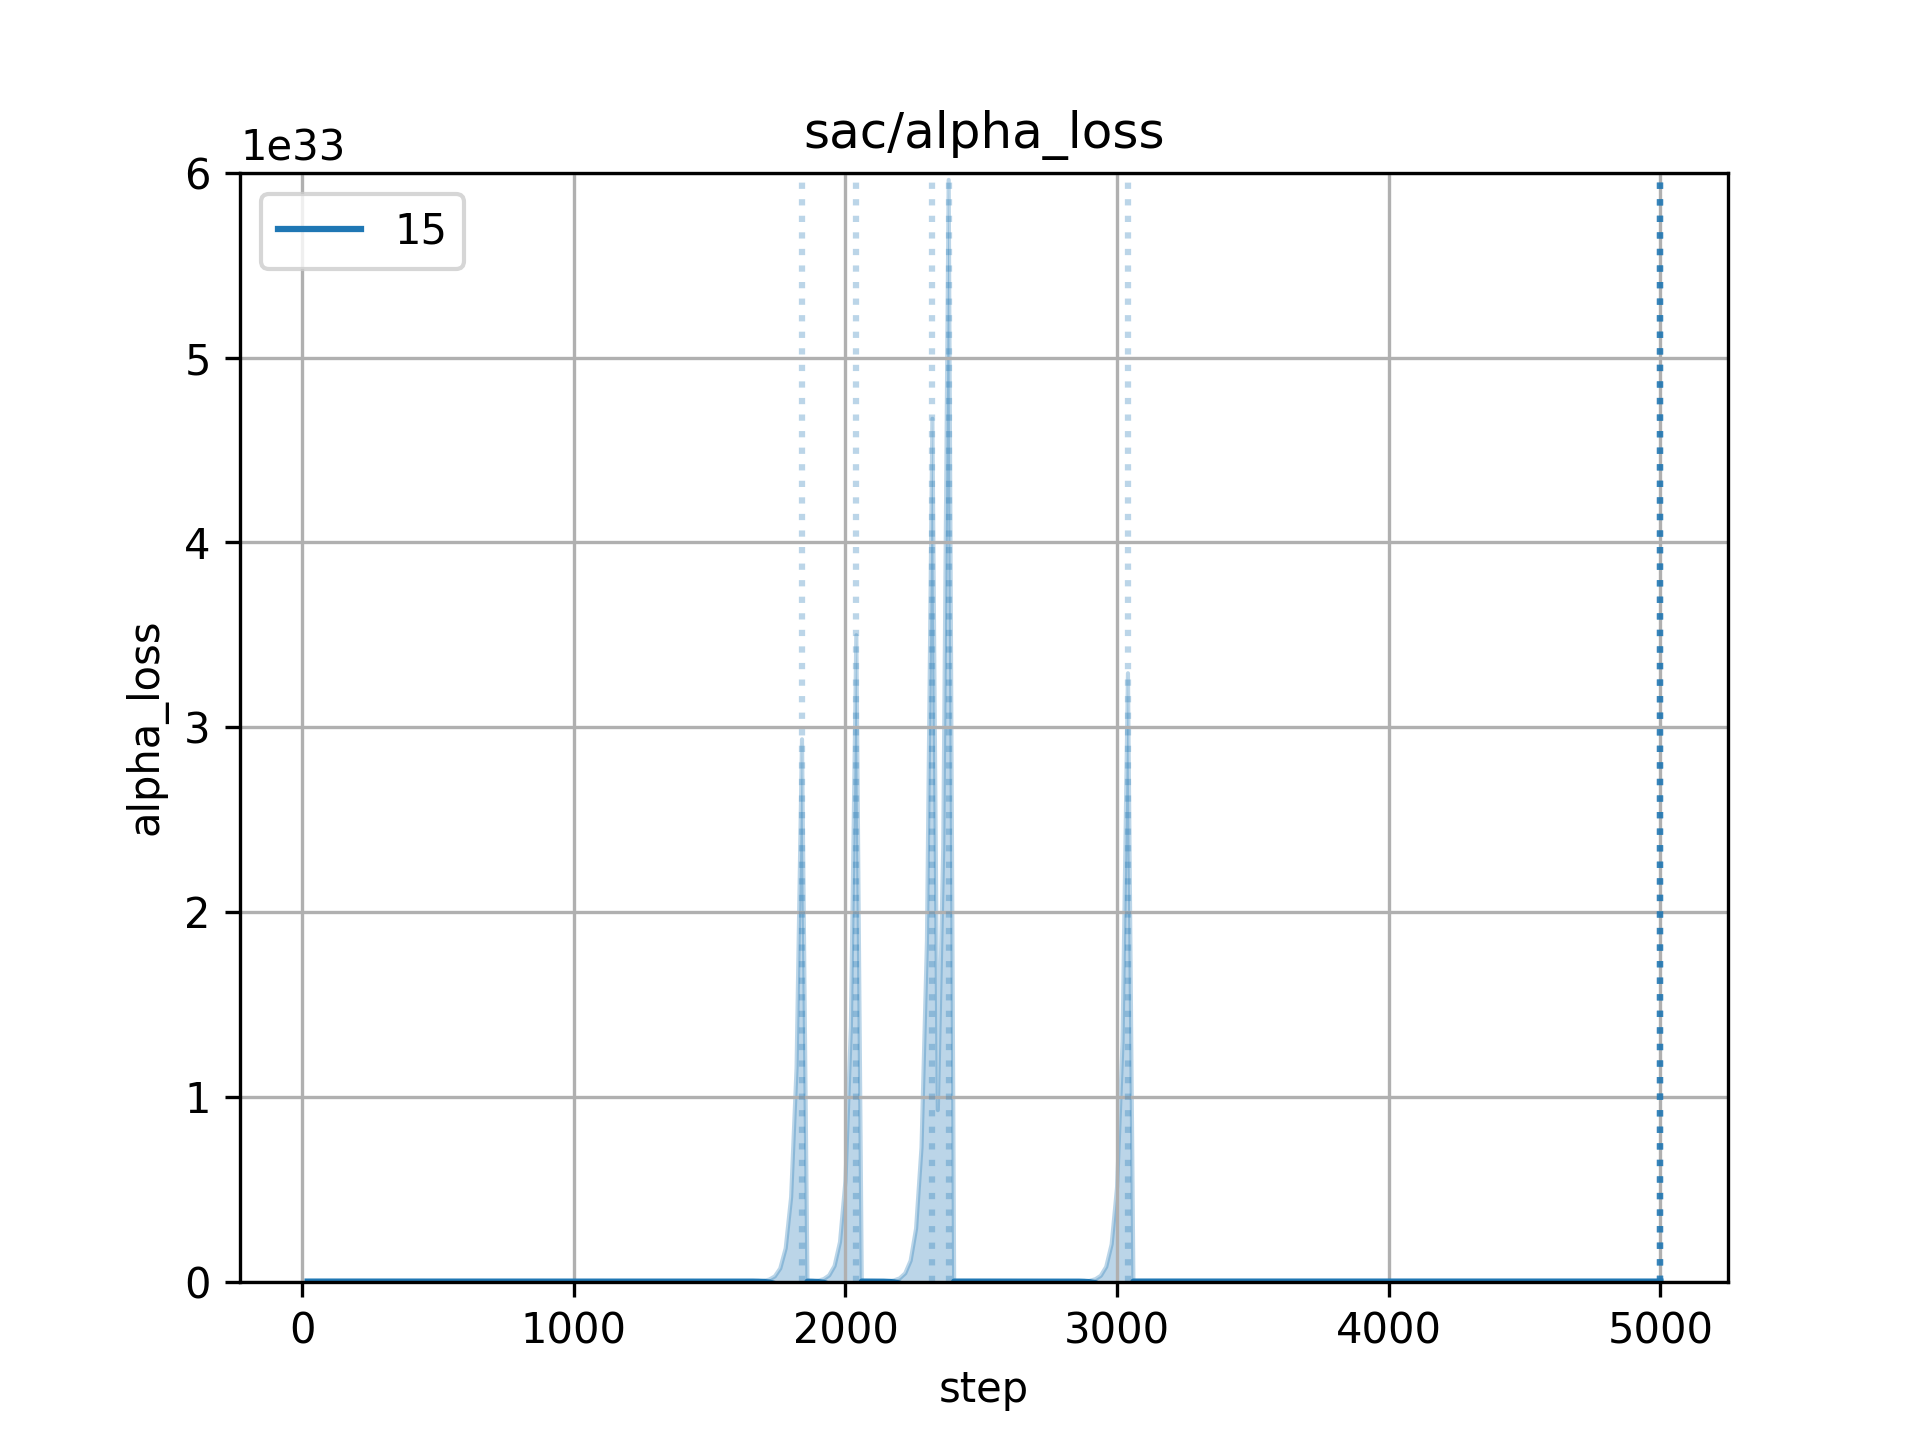
\includegraphics[width=0.5 \linewidth]{figures/appendix/alpha_loss_15.png}
    \end{center}
    \caption[alpha loss with $N = 15$]{Plot to show the correlation between training abortion and spike in alpha loss.}
    \label{fig:alpha_loss_15}
\end{figure}

\begin{figure}[h]
    \begin{center}
        \subfloat[$N = 2$]{
            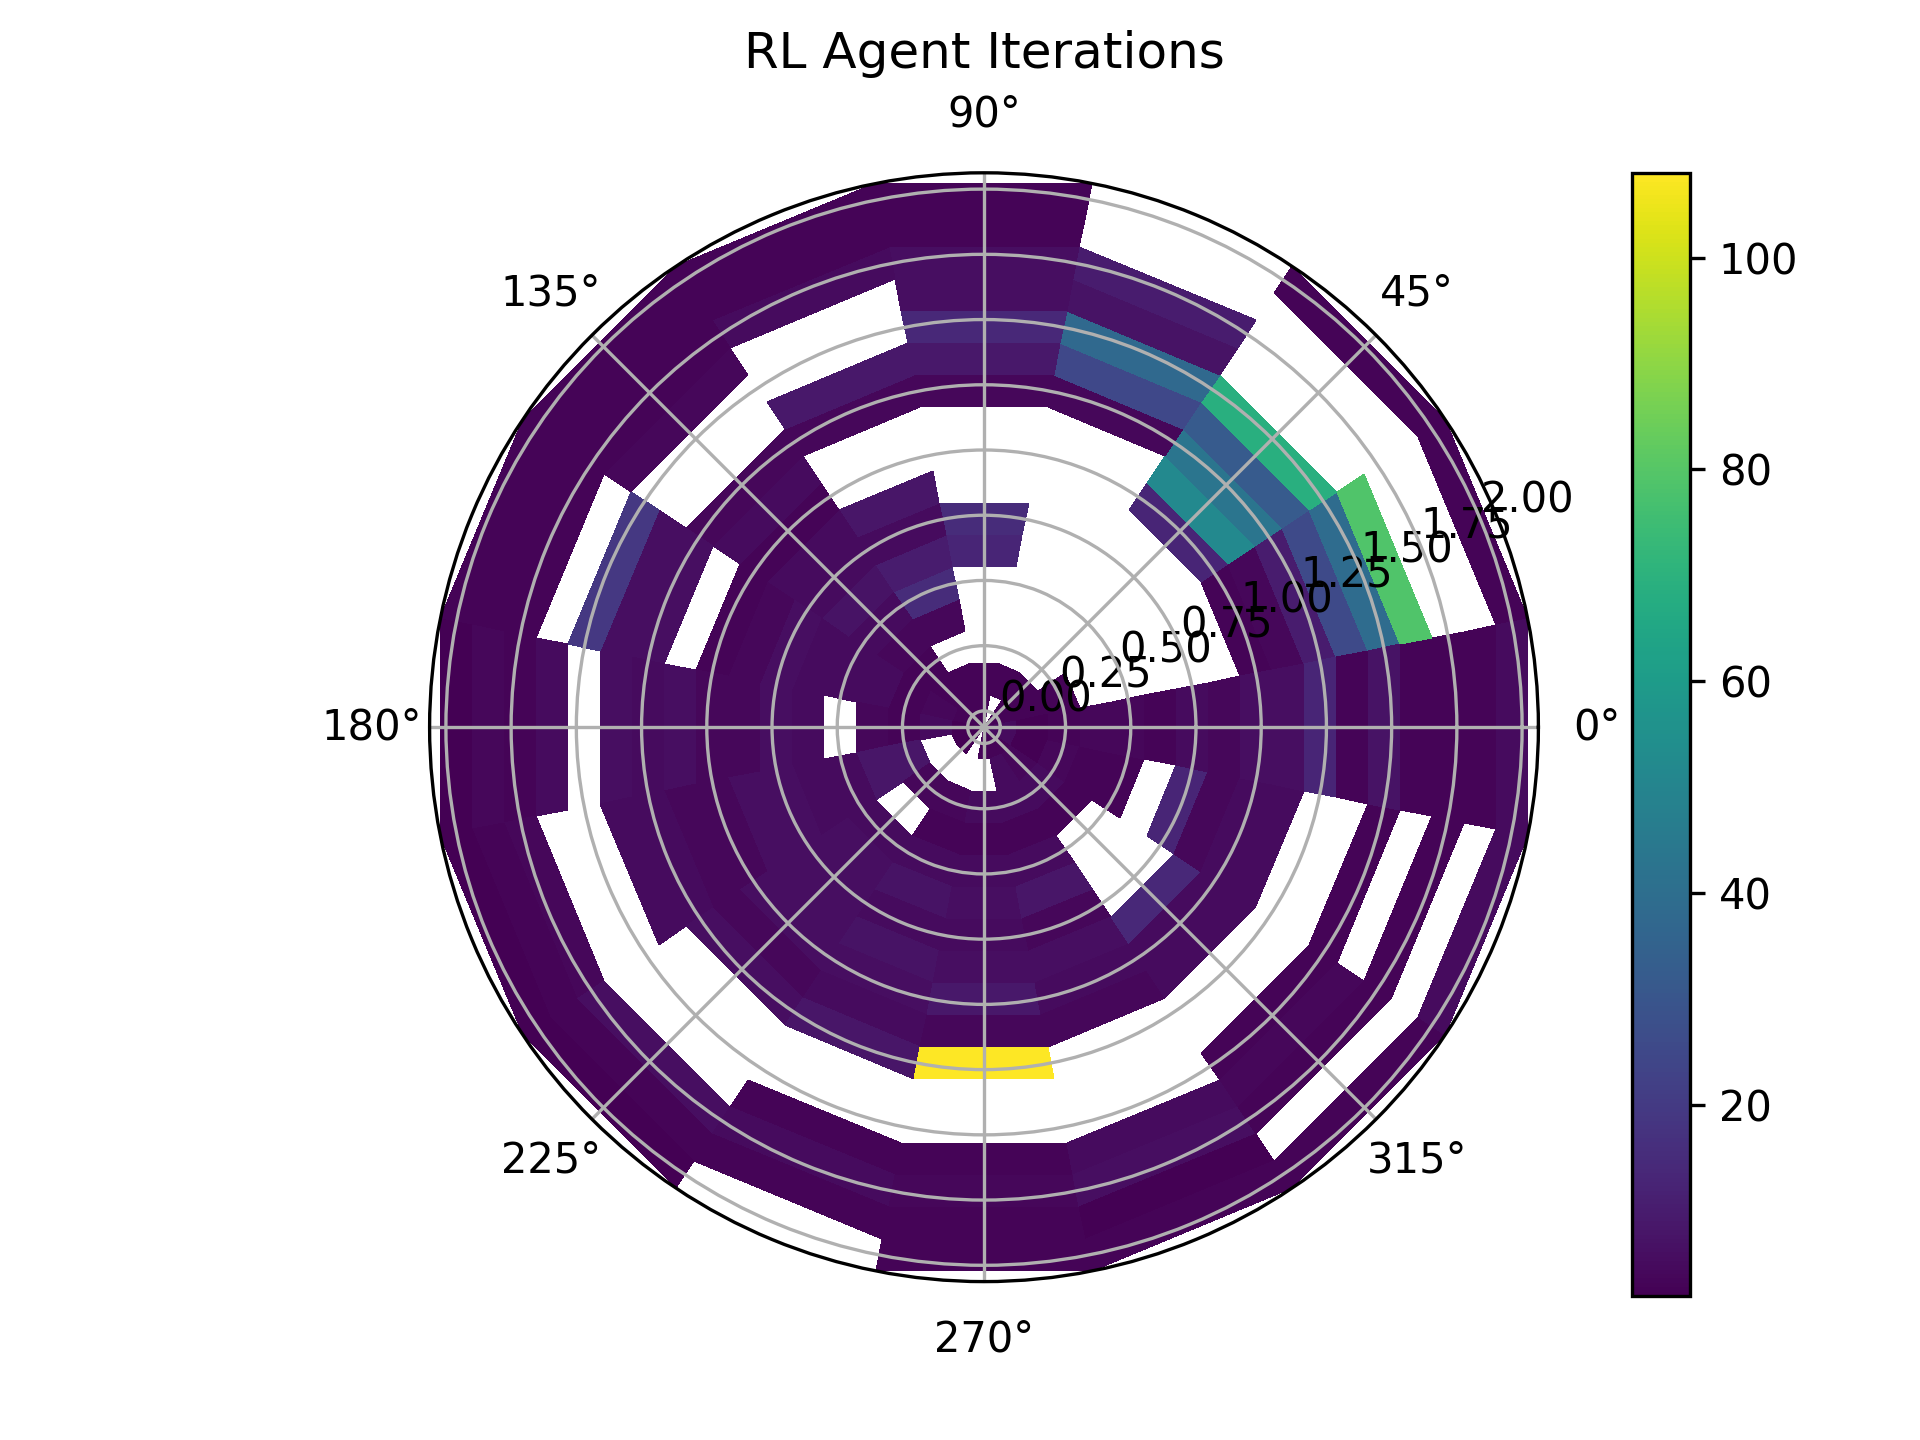
\includegraphics[width=0.46 \linewidth]{figures/experiments/RL_Agent_Iterations_baseline_2_1691621262_5000.png}
            \label{fig:RL_Agent_Target_Space_evaluation_baseline/2}
            }
        \hfill
        \subfloat[$N = 5$]{
            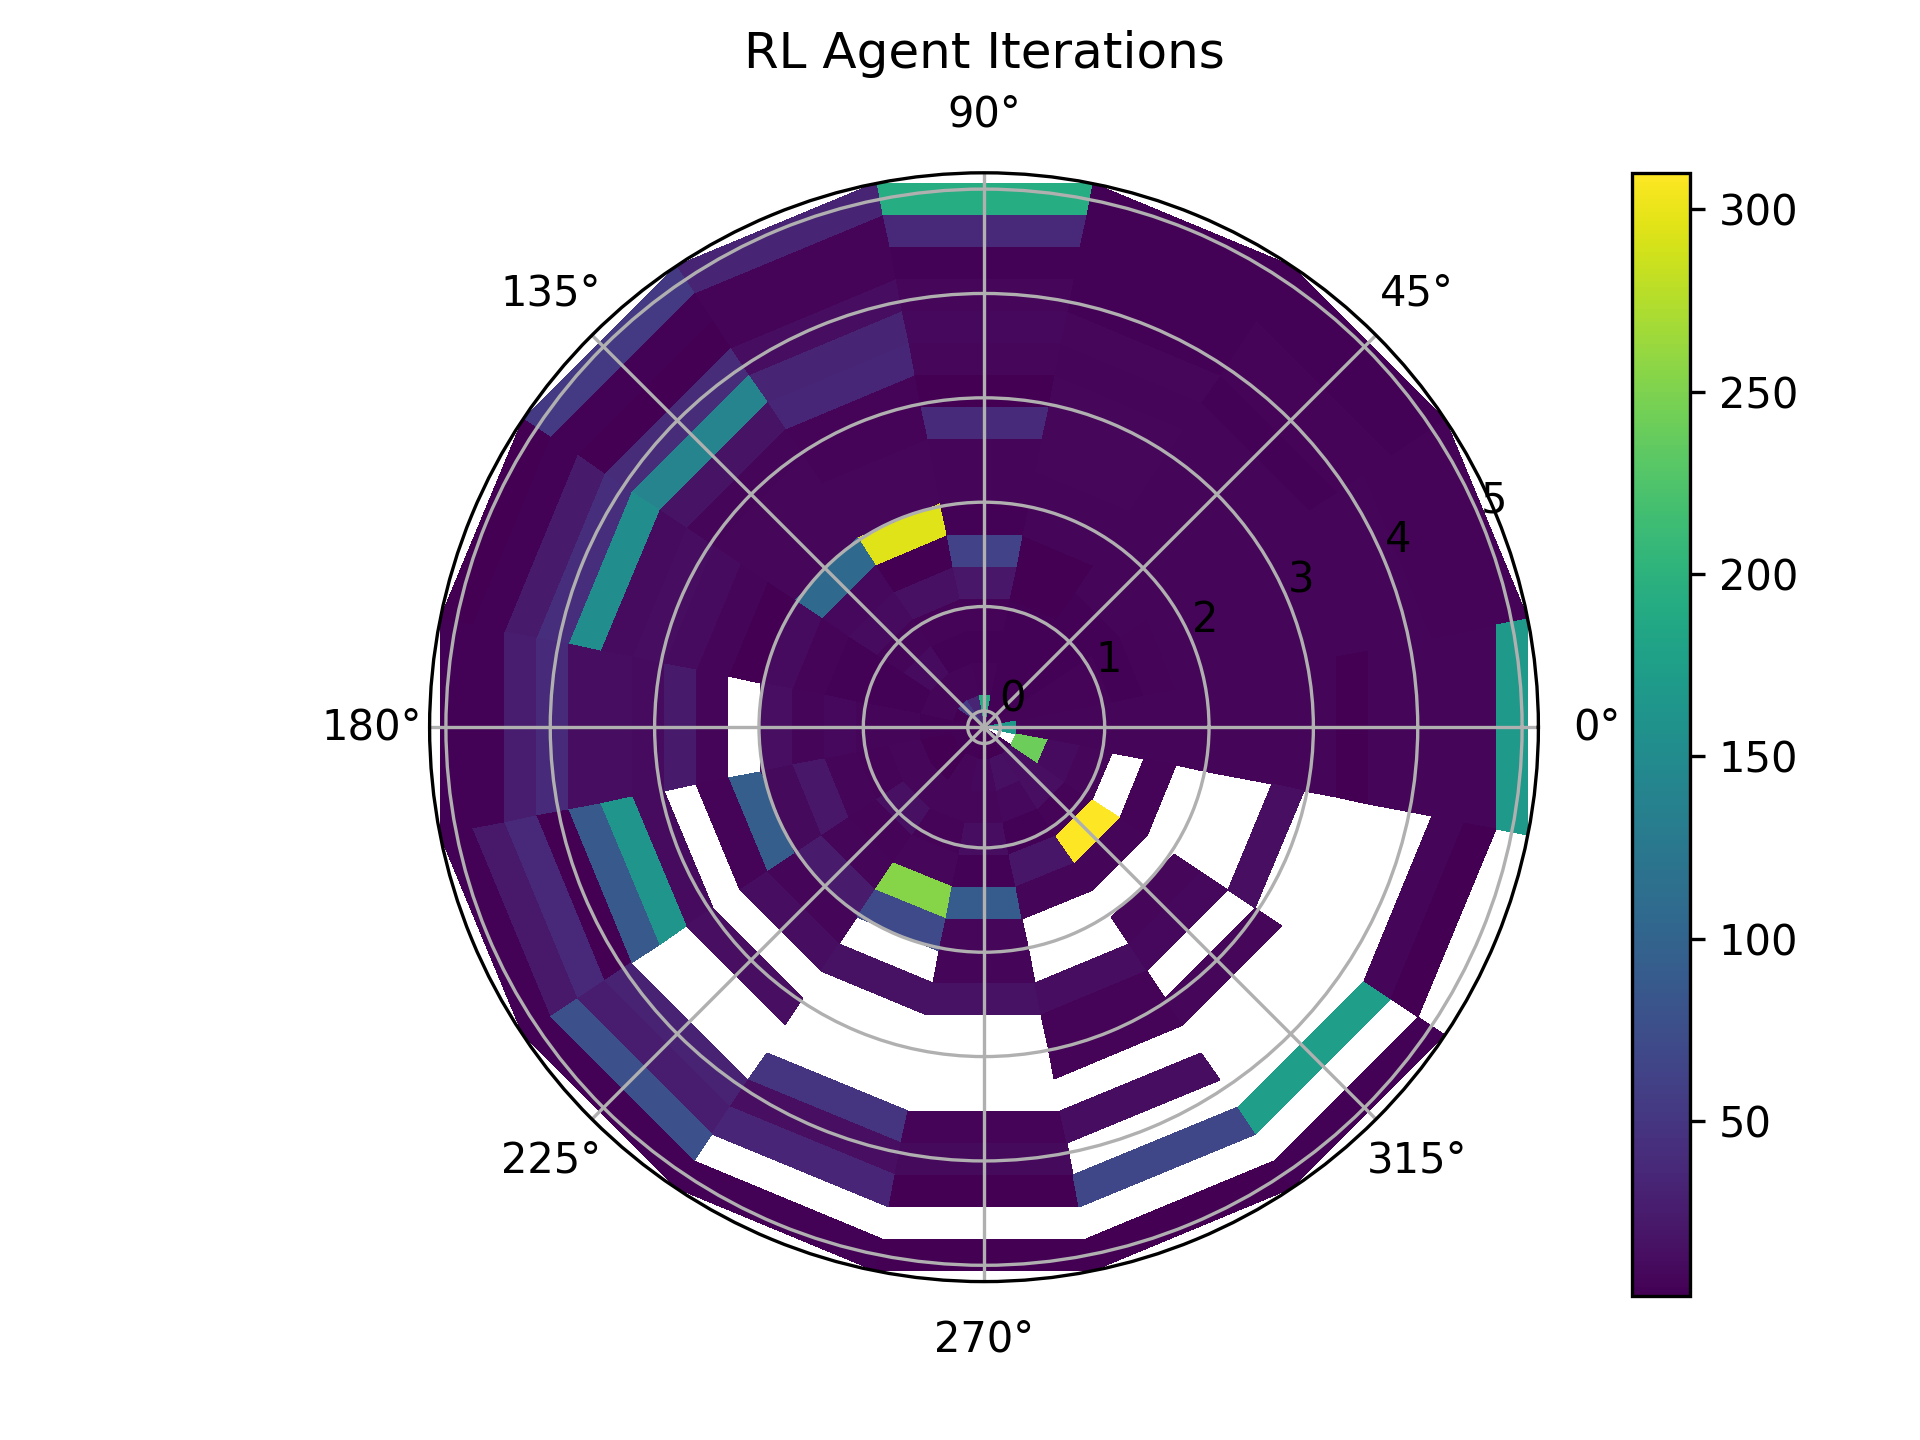
\includegraphics[width=0.46 \linewidth]{figures/experiments/RL_Agent_Iterations_baseline_5_1691621331_5000.png}
            \label{fig:RL_Agent_Target_Space_evaluation_baseline/5}
            }
        \\
        \subfloat[$N = 10$]{
            \includegraphics[width=0.46 \linewidth]{figures/experiments/RL_Agent_Iterations_baseline_10_1691618968_5000.png}
            \label{fig:RL_Agent_Target_Space_evaluation_baseline/10}
            }
        \hfill
        \subfloat[$N = 15$]{
            \includegraphics[width=0.46 \linewidth]{figures/experiments/RL_Agent_Iterations_baseline_15_1691619106_5000.png}
            \label{fig:RL_Agent_Target_Space_evaluation_baseline/15}
            }
        \\
        \subfloat[$N = 20$]{
            \includegraphics[width=0.46 \linewidth]{figures/experiments/RL_Agent_Iterations_baseline_20_1691619159_5000.png}
            \label{fig:RL_Agent_Target_Space_evaluation_baseline/20}
            }
    \end{center}
    \caption[RL Agent iteration evaluation baseline]{}
    \label{fig:RL_Agent_Target_Space_evaluation_baseline}
\end{figure}

\begin{figure}[h]
    \begin{center}
        \subfloat[$N = 2$]{
            \includegraphics[width=0.46 \linewidth]{figures/experiments/RL_Agent_Iterations_latent_actor_2_2_1693146377_5000.png}
            \label{fig:RL_Agent_Target_Space_evaluation_latent_2/2}
            }
        \hfill
        \subfloat[$N = 5$]{
            \includegraphics[width=0.46 \linewidth]{figures/experiments/RL_Agent_Iterations_latent_actor_2_5_1693146402_5000.png}
            \label{fig:RL_Agent_Target_Space_evaluation_latent_2/5}
            }
        \\
        \subfloat[$N = 10$]{
            \includegraphics[width=0.46 \linewidth]{figures/experiments/RL_Agent_Iterations_latent_actor_2_10_1693146420_5000.png}
            \label{fig:RL_Agent_Target_Space_evaluation_latent_2/10}
            }
        \hfill
        \subfloat[$N = 15$]{
            \includegraphics[width=0.46 \linewidth]{figures/experiments/RL_Agent_Iterations_latent_actor_2_15_1693146466_5000.png}
            \label{fig:RL_Agent_Target_Space_evaluation_latent_2/15}
            }
    \end{center}
    \caption[RL Agent iteration evaluation on VAE with latent = 2]{RL Agent iteration evaluation on VAE with latent = 2}
    \label{fig:RL_Agent_Target_Space_evaluation_latent_2}
\end{figure}

\begin{figure}[h]
    \begin{center}
        \subfloat[$N = 2$]{
            \includegraphics[width=0.46 \linewidth]{figures/experiments/RL_Agent_Iterations_latent_actor_4_2_1693063115_5000.png}
            \label{fig:RL_Agent_Target_Space_evaluation_latent_4/2}
            }
        \hfill
        \subfloat[$N = 5$]{
            \includegraphics[width=0.46 \linewidth]{figures/experiments/RL_Agent_Iterations_latent_actor_4_5_1693063141_5000.png}
            \label{fig:RL_Agent_Target_Space_evaluation_latent_4/5}
            }
        \\
        \subfloat[$N = 10$]{
            \includegraphics[width=0.46 \linewidth]{figures/experiments/RL_Agent_Iterations_latent_actor_4_10_1691620301_5000.png}
            \label{fig:RL_Agent_Target_Space_evaluation_latent_4/10}
            }
        \hfill
        \subfloat[$N = 15$]{
            \includegraphics[width=0.46 \linewidth]{figures/experiments/RL_Agent_Iterations_latent_actor_4_15_1691660318_5000.png}
            \label{fig:RL_Agent_Target_Space_evaluation_latent_4/15}
            }
    \end{center}
    \caption[RL Agent iteration evaluation on VAE with latent = 4]{RL Agent iteration evaluation on VAE with latent = 4}
    \label{fig:RL_Agent_Target_Space_evaluation_latent_4}
\end{figure}

\begin{figure}[h]
    \begin{center}
        \subfloat[$N = 2$]{
            \includegraphics[width=0.46 \linewidth]{figures/experiments/RL_Agent_Iterations_latent_actor_8_2_1691615359_3000.png}
            \label{fig:RL_Agent_Target_Space_evaluation_latent_8/2}
            }
        \hfill
        \subfloat[$N = 5$]{
            \includegraphics[width=0.46 \linewidth]{figures/experiments/RL_Agent_Iterations_latent_actor_8_5_1691612773_3000.png}
            \label{fig:RL_Agent_Target_Space_evaluation_latent_8/5}
            }
        \\
        \subfloat[$N = 10$]{
            \includegraphics[width=0.46 \linewidth]{figures/experiments/RL_Agent_Iterations_latent_actor_8_10_1691612526_3000.png}
            \label{fig:RL_Agent_Target_Space_evaluation_latent_8/10}
            }
        \hfill
        \subfloat[$N = 15$]{
            \includegraphics[width=0.46 \linewidth]{figures/experiments/RL_Agent_Iterations_latent_actor_8_15_1691626460_3000.png}
            \label{fig:RL_Agent_Target_Space_evaluation_latent_8/10}
            }
    \end{center}
    \caption[RL Agent iteration evaluation on VAE with latent = 8]{RL Agent iteration evaluation on VAE with latent = 8}
    \label{fig:RL_Agent_Target_Space_evaluation_latent_8}
\end{figure}


\begin{figure}[h]
    \begin{center}
        \subfloat[$N = 2$]{
            \includegraphics[width=0.46 \linewidth]{figures/experiments/RL_Agent_Iterations_latent_imitation_4_2_1693269830_3000.png}
            \label{fig:RL_Agent_Target_Space_evaluation_latent_8/2}
            }
        \hfill
        \subfloat[$N = 5$]{
            \includegraphics[width=0.46 \linewidth]{figures/experiments/RL_Agent_Iterations_latent_imitation_4_5_1693269853_3000.png}
            \label{fig:RL_Agent_Target_Space_evaluation_latent_8/5}
            }
        \\
        \subfloat[$N = 10$]{
            \includegraphics[width=0.46 \linewidth]{figures/experiments/RL_Agent_Iterations_latent_imitation_4_10_1693858660_3000.png}
            \label{fig:RL_Agent_Target_Space_evaluation_latent_8/10}
            }
        \hfill
        \subfloat[$N = 15$]{
            \includegraphics[width=0.46 \linewidth]{figures/experiments/RL_Agent_Iterations_latent_imitation_4_15_1693860185_3000.png}
            \label{fig:RL_Agent_Target_Space_evaluation_latent_8/10}
            }
    \end{center}
    \caption[RL Agent iteration evaluation on imitation VAE with latent = 8]{RL Agent iteration evaluation on imitation VAE with latent = 8}
    \label{fig:RL_Agent_Target_Space_evaluation_latent_8}
\end{figure}



\begin{figure}[h]
    \begin{center}
        \subfloat[$N = 2$]{
            \includegraphics[width=0.46 \linewidth]{figures/experiments/RL_Agent_Iterations_supervised_dist_loss_2_1693272467_3000.png}
            \label{fig:RL_Agent_Target_Space_evaluation_latent_8/2}
            }
        \hfill
        \subfloat[$N = 5$]{
            \includegraphics[width=0.46 \linewidth]{figures/experiments/RL_Agent_Iterations_supervised_dist_loss_5_1693272399_3000.png}
            \label{fig:RL_Agent_Target_Space_evaluation_latent_8/5}
            }
        \\
        \subfloat[$N = 10$]{
            \includegraphics[width=0.46 \linewidth]{figures/experiments/RL_Agent_Iterations_supervised_dist_loss_10_1694259480_3000.png}
            \label{fig:RL_Agent_Target_Space_evaluation_latent_8/10}
            }
    \end{center}
    \caption[RL Agent iteration evaluation on supervised model]{RL Agent iteration evaluation on supervised model}
    \label{fig:RL_Agent_Target_Space_evaluation_latent_8}
\end{figure}



\begin{figure}[h]
    \begin{center}
        \subfloat[$N = 2$]{
            \includegraphics[width=0.46 \linewidth]{figures/experiments/RL_Agent_Iterations_supervised_imitation_2_1693487256_3000.png}
            \label{fig:RL_Agent_Target_Space_evaluation_latent_8/2}
            }
        \hfill
        \subfloat[$N = 5$]{
            \includegraphics[width=0.46 \linewidth]{figures/experiments/RL_Agent_Iterations_supervised_imitation_5_1693487345_3000.png}
            \label{fig:RL_Agent_Target_Space_evaluation_latent_8/5}
            }
        \\
        \subfloat[$N = 10$]{
            \includegraphics[width=0.46 \linewidth]{figures/experiments/RL_Agent_Iterations_supervised_imitation_10_1693487396_3000.png}
            \label{fig:RL_Agent_Target_Space_evaluation_latent_8/10}
            }
    \end{center}
    \caption[RL Agent iteration evaluation on supervised imitation model]{RL Agent iteration evaluation on supervised imitation model}
    \label{fig:RL_Agent_Target_Space_evaluation_latent_8}
\end{figure}
    \newpage
    \thispagestyle{empty}
    \mbox{}


\end{document}
